\documentclass{article}
\usepackage[utf8]{inputenc}
\usepackage{polski}
\usepackage{amsmath,amssymb,graphicx,subfig,pdfpages,enumitem,empheq,verbatim,csvsimple}
\usepackage{multirow}

\author{Krystian Baran 145000}
\title{Sprawozdanie nr 2 od Lab 8 do Lab 14}

\begin{document}

\maketitle
\newpage

\tableofcontents
\newpage

\part{Laboratoria 07 - Estymacja punktowa}

Celem tych laboratoriów było zapoznanie się z metodami estymacji punktowej i wyznaczanie estymatorów metodą MM oraz NNW. MM to metoda momentów polegająca na wyznaczenie parametrów poprzez znajomości wzorów momentów rozkładu zależnych od parametrów. MNW to metoda największej wiarygodności w której wyznacza się funkcję wiarygodności i poszukuje się w których punktach osiąga ona maksimum, zatem sprowadza się do układu liniowego z pochodnymi częściowymi tej funkcji przyrównane do 0.

\section{Zadanie 1}
Wyznaczyć estymator parametru $p$ w rozkładzie Bernoulliego. \\ \par

Rozkład Bernoulliego ma rozkład następujący:
\[ P(X=k) = \binom{n}{k} p^k(1-p)^{n-k}, k = 0,1,\dots,n \]

Aby wyznaczyć estymator parametru $p$ skorzystamy z metody momentów. Dla rozkładu Bernoulliego $\mathbb{E}X = np$ i $\mathbb{D}^2(X) = np(1-p)$. Oznaczymy momenty punktowe jako:
\[ \mathbb{E}X = \overline{X} \]
\[ \mathbb{D}^2(X) = \frac{1}{n-1}\sum_{i=1}^n(X_i-\overline{X})^2 = s^2\]
Wtedy:
\begin{align*}
&\left\{
\begin{array}{l} np = \overline{X} \\ np(1-p) = s^2 \end{array} \right. \\ %\frac{1}{n-1}\sum_{i=1}^n(X_i-\overline{X})^2
&\left\{
\begin{array}{l} np = \overline{X} \\ \overline{X}(1-p) = s^2 \end{array} \right. \\ %\frac{1}{n-1}\sum_{i=1}^n(X_i-\overline{X})^2
&\left\{
\begin{array}{l} np = \overline{X} \\ 1-p = \frac{s^2}{\overline{X}} \end{array} \right. \\ %\frac{1}{\overline{X}(n-1)}\sum_{i=1}^n(X_i-\overline{X})^2
&\left\{
\begin{array}{l} np = \overline{X} \\ p =1 - \frac{s^2}{\overline{X}} \end{array} \right. \\ %\frac{1}{\overline{X}(n-1)}\sum_{i=1}^n(X_i-\overline{X})^2
&\left\{
\begin{array}{l} n = \frac{\overline{X}^2}{\overline{X}-s^2} \\ p = 1 - \frac{s^2}{\overline{X}} \end{array} \right. \\ %\frac{1}{\overline{X}(n-1)}\sum_{i=1}^n(X_i-\overline{X})^2
\end{align*}
Zatem estymator parametru $p$ jest $1 - \frac{s^2}{\overline{X}}$.

\newpage
\section{Zadanie 2}
Wyznaczyć MM oraz MNW estymatory parametrów rozkładu normalnego. \\ \par

Rozkład normalny definiowany jest w następujący sposób:
\[ N(\mu,\sigma)  = \frac{1}{\sigma\sqrt{2\pi}}e^{-\frac{(x-\mu)^2}{2\sigma^2}} \]
Parametr $\mu = \mathbb{E}X$ natomiast $\sigma = \mathbb{D}X$. Drugi moment zwykły tego rozkładu jest następujący:
\[ \mathbb{E}(X^2) = \sigma^2 + \mu^2 \]

Wyznaczymy estymatory parametrów metodą momentów. Niech $ \mathbb{E}X = \overline{X} $ i $\mathbb{E}(X^2) = \frac{\sum_{i=1}^n X_i^2}{n}$, wtedy:
\begin{align*}
& \left\{ 
\begin{array}{l}  \overline{X} = \mu \\  \frac{\sum_{i=1}^n X_i^2}{n} = \sigma^2 + \mu^2 \end{array} \right. \\
& \left\{ 
\begin{array}{l}  \overline{X} = \mu \\  \frac{\sum_{i=1}^n X_i^2}{n} = \sigma^2 + \overline{X}^2 \end{array} \right. \\
& \left\{ 
\begin{array}{l}  \overline{X} = \mu \\  \frac{\sum_{i=1}^n X_i^2}{n} = \sigma^2 + \mu^2 \end{array} \right. 
\end{align*}

Metodą największej wiarygodności natomiast potrzebujemy wyznaczyć funkcje wiarygodności.
\begin{align*}
L(x_1,x_2,\dots,x_n|\mu,\sigma) & = \prod_{i=1}^n \frac{1}{\sigma\sqrt{2\pi}}e^{-\frac{(x_i-\mu)^2}{2\sigma^2}} \\
& = \frac{1}{\sigma^n(2\pi)^{n/2}} e^{-\sum_{i=1}^n \frac{(x_i-\mu)^2}{2\sigma^2}} \\
\ln(L) & = -n\ln(\sigma) - \frac{n}{2}\ln(2\pi) - \sum_{i=1}^n \frac{(x_i-\mu)^2}{2\sigma^2}
\end{align*}

Obliczymy najpierw estymator parametru $\mu$.
\begin{align*}
\frac{\partial(\ln(L))}{\partial\mu} & = \sum_{i=1}^n \frac{2(x_i-\mu)}{2\sigma^2} \\
& = \frac{\sum_{i=1}^n (x_i-\mu)}{\sigma^2} = 0 \\
\sum_{i=1}^n (x_i-\mu) & = 0 \\
\sum_{i=1}^n x_i - n\mu & = 0 \\
\mu & = \frac{\sum_{i=1}^n x_i}{n}
\end{align*}

Dla parametru $\sigma$ natomiast:
\begin{align*}
\frac{\partial(\ln(L))}{\partial\sigma} & = -\frac{n}{\sigma} + \sum_{i=1}^n \frac{2(x_i-\mu)^2}{2\sigma^3} \\
& = -\frac{n}{\sigma} + \frac{\sum_{i=1}^n (x_i-\mu)^2}{\sigma^3} = 0 \\
\frac{\sum_{i=1}^n (x_i-\mu)^2}{\sigma^3} & = \frac{n}{\sigma} \\
\frac{\sum_{i=1}^n (x_i-\mu)^2}{n} & = \sigma^2 \\
\sigma & = \sqrt{\frac{\sum_{i=1}^n (x_i-\mu)^2}{n}}
\end{align*}

Widzimy zatem że parametry $\mu$ i $\sigma$ są, odpowiednio, średnią i odchyleniem standardowym populacji szeregu punktowego.

\newpage
\section{Zadanie 3}
Wyznaczyć MNW estymator parametru rozkładu Poissona. \\ \par

Rozkład Poissona definiowany jest w następujący sposób:
\[ P(X = k) = \frac{\lambda^k e^{-\lambda}}{k!}, k = 0,1,2,\dots \]

Jest to rozkład jedno parometrowy. Aby wyliczyć estymator parametru $\lambda$ potrzebujemy obliczyć funkcję wiarygodności.
\begin{align*}
L(k_1,k_2,\dots,k_n|\lambda) & = \prod_{i=1}^n P(X = k_i) = \prod_{i=1}^n \frac{\lambda^{k_i} e^{-\lambda}}{k_i!} \\
& = \lambda^{\sum_{i=1}^n k_i} e^{-n\lambda} \prod_{i=1}^n \frac{1}{k_i!} \\
\ln(L) & = \ln(\lambda)\sum_{i=1}^n k_i - n\lambda - \sum_{i=1}^n \ln{k_i!}
\end{align*}

Estymator parametru jest maksimum tej funkcji po zmiennej $\lambda$, zatem przyrównamy pierwszą pochodną do zera i znajdziemy szukany estymator.
\begin{align*}
\frac{\partial(\ln(L))}{\partial\lambda} & = \frac{\sum_{i=1}^n k_i}{\lambda} - n = 0 \\
n & = \frac{\sum_{i=1}^n k_i}{\lambda} \\
\lambda & = \frac{\sum_{i=1}^n k_i}{n}
\end{align*}
Sprawdzimy teraz drugą pochodną.
\[ \begin{array}{cr} \frac{\partial^2(\ln(L))}{\partial\lambda^2} = -\frac{\sum_{i=1}^n k_i}{\lambda^2} < 0, & \forall \lambda \end{array} \]

Zatem estymator parametru $\lambda$ jest średnia arytmetyczna populacji.

\newpage
\section{Zadanie 4}
Celem sprawdzenia dokładności wskazań pewnego przyrządu pomiarowego dokonano 10
pomiarów tej samej wielkości fizycznej $X$ i otrzymano następujące wyniki: \\
\begin{center}
9,01; 9,00; 9,02; 8,99; 8,98; 9,00; 9,00; 9,01; 8,99; 9,00.
\end{center}
Dokonać przekształcenia pomiarów według wzoru:
\[ Y = 100(X - 9) \]
Dla wielkości $X$ i $Y$ oszacować ich wartości oczekiwane i wariancje. \\ \par

Na początku sporządzimy tabele wartości $X$ i $Y$ korzystając z podanego wzoru.
\begin{center}
\begin{tabular}{|c|c|c|}
\hline
Lp. & X & Y \\ \hline
1 & 9.01	& 1 \\ \hline
2& 9 &	0 \\ \hline
3 &9.02	& 2 \\ \hline
4 & 8.99	& -1\\ \hline
5 & 8.98	& -2\\ \hline
6 & 9	 &0\\ \hline
7 & 9	&0\\ \hline
8 & 9.01	&1\\ \hline
9 & 8.99	&-1\\ \hline
10 & 9	&0\\ \hline
\end{tabular}
\end{center}
Oszacujemy wartość oczekiwaną jako średnia z podanych wartości, czyli:
\[ \mathbb{E}X = \overline{X} = \frac{\sum x_i}{n} = \frac{90}{10} = 9 \]
\[ \mathbb{E}Y = \overline{Y} = \frac{\sum y_i}{n} = \frac{9}{10} = 0 \]

Aby obliczyć odchylenie standardowe potrzebujemy sumę kwadratów obniżonych o średnią.
\begin{center}
\begin{tabular}{|c|c|c|}
\hline
Lp. & $(x_i - \overline{X})^2$ & $(y_i - \overline{Y})^2$ \\ \hline
1 & 0.0001	 & 1 \\ \hline
2 & 0.0000	 & 0 \\ \hline
3 & 0.0004	 & 4 \\ \hline
4 & 0.0001	 & 1 \\ \hline
5 & 0.0004	 & 4 \\ \hline
6 & 0.0000	 & 0 \\ \hline
7 & 0.0000	 & 0 \\ \hline
8 & 0.0001	 & 1 \\ \hline
9 & 0.0001	 & 1 \\ \hline
10 & 0.0000 & 0 \\ \hline
SUM & 0.0012 & 12 \\ \hline
\end{tabular}
\end{center}

Wtedy można łatwo obliczyć wartość odchylenia standardowego:
\[ \sigma_x = \sqrt{\frac{\sum (x_i - \overline{X})^2}{n}} = \sqrt{\frac{0.0012}{10}} \approx 0.010954451 \]
\[ \sigma_y = \sqrt{\frac{\sum (y_i - \overline{Y})^2}{n}} = \sqrt{\frac{12}{10}} \approx 1.095445115 \]

Wartość oczekiwana zmiennej $X$ wynosi 9, gdzie $X$ jest mierzona długość, więc możemy przyjąć że jest to długość mierzonego obiektu.\\
Wartość oczekiwana zmiennej $Y$, która wskazuje nam błąd procentowy względem wartości rzeczywistej 9, wynosi 0; zatem obiekt zmierzony został poprawnie. \\ \par
Odchylenie standardowe zmiennej $X$ wynosi w przybliżeniu 0.01, oznacza to że rzeczywistsza długość obiektu, z uwzględnieniem błędu pomiarowego wynosi $9.00 \pm0.01$.\\
Odchylenie standardowe zmiennej $Y$ wynosi w przybliżeniu 1, zatem rzeczywista wartość procentowego błędu jest $\pm1\%$.

\newpage
\section{Zadanie 5}
Wygenerować 50 elementową próbę prostą z populacji, w której cecha $X$ ma rozkład o gęstości $f(x) = \frac{x}{8} \textbf{1}_{(0;4)}(x)$
\begin{enumerate}[label = \alph*)]
\item Sporządzić histogram.
\item Wyznaczyć wartość oczekiwaną i wariancję oraz ich oceny na podstawie wygenerowanej próby.
\end{enumerate}

\subsection{a)}
Aby wygenerować próbę korzystając z twierdzenia obrócenia dystrybuanty musimy obliczyć dystrybuantę
\begin{align*}
F_X(x) & = \int_\mathbb{R}  \frac{t}{8} \textbf{1}_{(0;4)}(t) dt = \int_0^x \frac{t}{8} dt \\
& = \frac{t^2}{16} \Big\vert_0^x \\
& = \frac{x^2}{16}
\end{align*}
Zatem dystrybuanta jest następująca:
\[ F_X(x) = \left\{ \begin{array}{lcc} 0 & , & x\leq 0 \\ \frac{x^2}{16} & , & 0<x<4 \\ 1 & , & x \geq 4 \end{array} \right. \]
Odwrócimy dystrybuantę.
\begin{align*}
y & = \frac{x^2}{16} \\
16y & = x^2 \\
x & = 4\sqrt{y}
\end{align*}
Poniżej przedstawiony został histogram przedziałowy wygenerowanej próby:
\begin{figure}[h!]
\begin{center}
\includegraphics[height = 0.4\textheight, angle = 0]{"lab7zad5.png"}
\end{center}
\end{figure}

\subsection{b)}
Obliczymy teraz wartość oczekiwaną i wariancję z podanej funkcji i z wygenerowanej próby:
\begin{align*}
\mathbb{E}X & = \int_\mathbb{R} \frac{x^2}{8}\mathbb{I}_{(0,4)}(x) dx = \int_0^4 \frac{x^2}{8} dx \\
& = \frac{x^3}{24} \Big\vert_0^4 \\
& = \frac{64}{24} \approx 2.666666667
\end{align*}

\begin{align*}
\mathbb{E}(X^2) & = \int_\mathbb{R} \frac{x^3}{8}\mathbb{I}_{(0,4)}(x) dx = \int_0^4 \frac{x^3}{8} dx \\
& = \frac{x^4}{32} \Big\vert_0^4 \\
& = \frac{64}{32} = 8
\end{align*}

\[ \mathbb{D}^2(X) = \mathbb{E}(X^2) - \mathbb{E}X^2 = 8 - \frac{4096}{576} \approx 0.88888888889 \]

Wartość oczekiwana z próby będzie średnią z próby, natomiast wariancje oznaczymy następującym wzorem:
\[ s^2 = \frac{1}{n-1}\sum_{i=1}^n (x_i - \overline{X})^2 \]

Obliczymy szukane wartości w R, gdzie \textit{prob} jest tablicą zawierającą 50-elementową próbę.
\[ \overline{X} \overset{R}{=} mean(prob) \approx 2.751196 \]
\[ s^2 \overset{R}{=} var(prob) \approx 0.8295317 \]
Widzimy że że oba wartości są do siebie blisko, zatem możemy stwierdzić że obliczyliśmy poprawnie, gdzie $\overline(X) = 2.7 \pm 0.1$ i $s^2 = 0.8 \pm 0.1$.

% Lab 7 Zadanie 6
\newpage
\section{Zadanie 6}
Korzystając z dostępnego oprogramowania wygenerować 100 elementową próbę według rozkładu
\begin{enumerate}[label = \alph*)]
\item bin(20; 0,8),
\item nbin(3;0,1),
\item Poisson(5).
\end{enumerate}
Sporządzić histogram i dokonać ocenę punktową parametrów. \\ \par

\subsection{a)}
Aby wygenerować losową próbę 100 elementową rozkładu Dwumianowego skorzystamy z funkcji R-owskiej \textit{rbinom()}. Poniżej przestawiony został histogram dla losowej próby.
\begin{figure}[h!]
\begin{center}
\includegraphics[height = 0.4\textheight, angle = 0]{"lab7zad6_a.png"}
\end{center}
\end{figure}

Wartość oczekiwana i wariancja teoretyczna wynoszą:
\[ \mathbb{E}(X) = np = 20\cdot0.8 = 16 \]
\[ \mathbb{D}^2(X) = np(1-p) = 20\cdot 0.8\cdot 0.2 = 3.2 \]

Natomiast, korzystając z wygenerowanej próby i z funkcji na średnią i wariancje w R otrzymujemy następujące wartości:
\[ \overline{X} \overset{R}{=} mean(prob) \approx 15.87 \]
\[ s^2 \overset{R}{=} var(prob) \approx 3.104141 \]

Widzimy że wartości tę są blisko wartości teoretycznej, zatem można stwierdzić że estymowana wartość oczekiwana wynosi $16 \pm 0.2$ a wariancja wynosi $3.1 \pm 0.1$.

\subsection{b)}
Podobnie jak w podpunkcie \textbf{a} wygenerujemy losową próbę 100-elementową w R za pomocą funkcji wbudowanej \textit{rnbinom()}. Poniżej przedstawiono histogram.
\begin{figure}[h!]
\begin{center}
\includegraphics[height = 0.4\textheight, angle = 0]{"lab7zad6_b.png"}
\end{center}
\end{figure}

Wartość oczekiwana i wariancja teoretyczna wynoszą:
\[ \mathbb{E}(X) = \frac{(1-p)r}{p} = \frac{3\cdot0.9}{0.1} \approx 27 \]
\[ \mathbb{D}^2(X) = \frac{(1-p)r}{p^2} = \frac{3\cdot0.9}{0.01} \approx 270 \]

Natomiast, korzystając z wygenerowanej próby i z funkcji na średnią i wariancje w R otrzymujemy następujące wartości:
\[ \overline{X} \overset{R}{=} mean(prob) \approx 27.75 \]
\[ s^2 \overset{R}{=} var(prob) \approx 216.8965 \]

Dla wartości oczekiwanej widzimy że wartości tę są blisko wartości teoretycznej, zatem można stwierdzić że estymowana wartość oczekiwana wynosi $27 \pm 0.7$. Natomiast wariancja jest znacznie inna niż wartość teoretyczna; może wynikać to z tego że dla dużych wartości nie uzyskujemy znaczną dokładność, zatem na pewno pierwsza liczba została obliczona dokładnie a reszta już nie.

\subsection{c)}
Podobnie jak w podpunkcie \textbf{a} i \textbf{b} wygenerujemy losową próbę 100-elementową w R za pomocą funkcji wbudowanej \textit{rpois()}. Poniżej przedstawiono histogram.
\begin{figure}[h!]
\begin{center}
\includegraphics[height = 0.4\textheight, angle = 0]{"lab7zad6_c.png"}
\end{center}
\end{figure}

Wartość oczekiwana i wariancja teoretyczna wynoszą:
\[ \mathbb{E}(X) = \lambda = 5 \]
\[ \mathbb{D}^2(X) = \lambda = 5 \]

Natomiast, korzystając z wygenerowanej próby i z funkcji na średnią i wariancje w R otrzymujemy następujące wartości:
\[ \overline{X} \overset{R}{=} mean(prob) \approx 4.59 \]
\[ s^2 \overset{R}{=} var(prob) \approx 4.870606 \]

W tym przypadku widzimy że przy aproksymacji do liczby całkowitej uzyskamy dobrą wartość estymowanych parametrów. Zatem uznajemy że estymowana wartość oczekiwana wynosi $5 \pm 1$ a wariancja tak samo.

\newpage
\section{Zadanie 7}
Wygenerować 100 elementową próbę według rozkładu logarytmiczno-normalnego z parametrami $\mu = 2.3$ i $\sigma = 0.5$.
\begin{enumerate}[label = \alph*)]
\item Sporządzić histogram.
\item Dokonać estymacji parametrów, ocenić wartość oczekiwaną i wariancję oraz porównać te wartości z wartościami teoretycznymi.
\end{enumerate}

Aby wygenerować losową próbę 100-elementową skorzystamy z dostępnej funkcji R-owskiej dla rozkładu logarytmiczno-normalnego \textit{rlnorm()}. Poniżej przedstawiony został histogram z wygenerowanej próby:
\begin{figure}[h!]
\begin{center}
\includegraphics[height = 0.4\textheight, angle = 0]{"lab7zad7.png"}
\end{center}
\end{figure}

Dla rozkładu logarytmiczno-normalnego wartość oczekiwana i wariancja są następujące:
\[ \mathbb{E}(X) = e^\mu = e^2.3 \approx 9.974182455 \]
\[ \mathbb{D}^2(X) = (e^{\sigma^2} - 1)e^{2\mu+\sigma^2} = (e^{0.25}-1)e^{4.6 + 0.25} \approx 36.28151745 \]

Korzystając z wygenerowanej próby i z funkcji na średnią i wariancje w R otrzymujemy następujące wartości:
\[ \overline{X} \overset{R}{=} mean(prob) \approx 11.72756 \]
\[ s^2 \overset{R}{=} var(prob) \approx 30.83267 \]

Wartości te różnią się nie wiele od wartości teoretycznych.

\newpage
% Laboratoria 8 
\part{Laboratoria 8 - Estymacja przedziałowa}
Celem tych laboratoriów było zapoznanie się z metodami estymacji parametrów dla danych przedziałowych. Zapoznaliśmy się także z wyznaczaniem przedziałów ufności dla wartości oczekiwanej oraz wariancji.

% Lab 8 - Zadanie 2
\section{Zadanie 2}
Korzystając z dostępnego oprogramowania wybrać rozkład i wygenerować małą oraz dużą próbę i na ich podstawie dokonać estymacji punktowej przedziałowej parametrów. \\ \par

Niech prędkość wiatru w danej miejscowości ma rozkład Weibulla z danymi parametrami $k=2$ i $\lambda = 8$ i niech mała próba losowa będzie się składać z 20 elementów, natomiast duża próba będzie zawierała 100 elementów. n-elementowa próba rozkładu Weibulla została wykonana z pomocą funkcji R-owskiej \textit{rweibull()}.

\subsection{20 - elementów}
Poniżej przedstawiono tabele przedziałową próby.
\begin{center}
\csvreader[tabular = |c|c|c|,
table head = \hline \bfseries{Lp} & \bfseries{Przedz} & \bfseries{Licz} \\ \hline,
late after last line = \\ \hline]{w8zad2_a.csv}{}{\csvlinetotablerow}
\end{center}

Aby obliczyć średnią korzystaliśmy ze wzoru poniżej, gdzie $x_i$ jest środkiem przedziału. $n_i$ natomiast jest liczebnością przedziału.
\[ \overline{X} = \frac{\sum_{i=1}^n x_i \cdot n_i}{n} = \frac{152}{20} \approx 7.6\]

Natomiast dla wariancji skorzystaliśmy ze wzoru poniżej.
\[ S^2_n = \frac{\sum_{i=1}^n(x_i-\overline{X})^2 \cdot n_i}{n-1} = \frac{256.8}{19} \approx 13.51578947 \]

\subsection{100 - elementów}
Poniżej przedstawiono tabele przedziałową próby.
\begin{center}
\csvreader[tabular = |c|c|c|,
table head = \hline \bfseries{Lp} & \bfseries{Przedz} & \bfseries{Licz} \\ \hline,
late after last line = \\ \hline]{w8zad2_b.csv}{}{\csvlinetotablerow}
\end{center}

Jak w podpunkcie \textbf{a} obliczono, odpowiednio, średnią i wariancję.
\[ \overline{X} = \frac{768}{100} \approx 7.68 \]
\[ S^2_n = \frac{1689.76}{99} \approx 17.06828283 \]

Widzimy zatem że przy zwiększeniu próby uzyskaliśmy tylko lekką poprawę wartości średniej, natomiast wariancje znacznie różnią się od siebie.

\newpage
% Lab 8 - Zadanie 3
\section{Zadanie 3}
Rozkład wyników pomiarów głębokości morza w pewnym rejonie jest normalny. Dokonano 5 niezależnych pomiarów głębokości morza w tym rejonie i otrzymano następujące wyniki (w [m]): 871, 862, 870, 876, 866. Na poziomie ufności 0,90 wyznaczyć CI dla wartości oczekiwanej oraz dla wariancji głębokości morza w badanym rejonie. \\ \par

Obliczymy najpierw średnią i wariancję z podanej próby:
\[ \overline{X}_5 = \frac{1}{n}\sum_{i=1}^n X_i = \frac{4345}{5} = 869 \]
\[ S^2_5 = \frac{1}{n-1}\sum_{i=1}^n (X_i-\overline{X})^2 = \frac{112}{4} = 28 \]
\[ S_5 = \sqrt{S_5^2} \approx 5.291502622 \]

Wyznaczymy teraz $\alpha$ wiedząc że poziom ufności jest 0.90.
\[1-\alpha = 0.90 \Rightarrow \alpha = 0.1 \]

Ponieważ pomiary głębokości morza mają rozkład normalny gdzie nie znane są parametry $m$ i $\sigma$ skorzystamy najpierw z przedziału ufności dla $\sigma^2$ podany poniżej:
\[R = \Big( \frac{(n-1)S_n^2}{\chi_{1-\frac{\alpha}{2}; n-1}^2} ; \frac{(n-1)S_n^2}{\chi_{\frac{\alpha}{2}; n-1}^2} \Big) \]

Obliczymy teraz wartości kwantyli rozkładu $\chi^2$:
\[ \chi_{1-0.05; 4}^2 \overset{R}{=} qchisq(0.95, 4) \approx 9.487729 \]
\[ \chi_{0.05; 4}^2 \overset{R}{=} qchisq(0.05, 4) \approx 0.710723 \]

Wtedy szukany przedziały ufności dla $\sigma^2$:
\[R = (11.80472166; 157.5860075) \]

Teraz możemy obliczyć przedziały ufności dla wartości oczekiwanej z poniższego wzoru:
\[ \overline{X}_n \mp t_{1-\frac{\alpha}{2};n-1} \frac{S_n}{\sqrt{n}} \]

$t_{1-\frac{\alpha}{2};n-1}$ to kwantyl rozkładu Studenta z $n-1$ stopniami swobody.
\[ t_{0.95;4} \overset{R}{=} qt(0.95,4) \approx 2.131847 \]

Wtedy szukany przedział to:
\[R = (863.9551292; 874.0448708) \] 

\newpage
% Lab 8 - Zadanie 5
\section{Zadanie 5}
Linia lotnicza chce oszacować frakcję Polaków, którzy będą korzystać z nowo otwartego połączenia między Poznaniem a Londynem. Wybrano losową próbę 347 pasażerów korzystających z tego połączenia, z których 201 okazało się Polakami.
\begin{enumerate}[label = \alph*)]
\item Wyznaczyć 90\% przedział ufności dla frakcji Polaków wśród pasażerów korzystających z nowo otwartego połączenia.
\item Wygenerować 347 elementową próbę według rozkładu $B(0,58)$ identyfikującą polskich pasażerów i na tej podstawie wyznaczyć 90\% przedział ufności.
\end{enumerate}

\subsection{a)}
Wyznaczmy $\alpha$ widząc ze szukamy przedział ufności 90\%.
\[ 1 - \alpha = 0.9 \Rightarrow \alpha = 0.1 \]

Niech każdy pasażer ma narodowość niezależną od innych pasażerów, wtedy każdy pasażer $X_i$ będzie miał rozkład Bernouilliego z nieznanym parametrem $p$ opisując czy jest polakiem czy nie. Zatem $X = \sum X_i$ będzie także rozkładem Bernoulliego i będzie opisywało liczbę polaków z pośród pasażerów. \\
Aby wyznaczyć przedział ufności dla parametru $p$ sprawdzimy poniższy warunek:
\[ 1 < \overline{p}_n \mp 3\sqrt{\frac{\overline{p}_n(1-\overline{p}_n) }{n}} < 1 \]
\[ \overline{p}_n \mp 3\sqrt{\frac{\overline{p}_n(1-\overline{p}_n}{n}) } = \frac{201}{347} \mp 3\sqrt{\frac{201/347\cdot 146/347}{347}} \approx 0.579251 \mp 0.079506 \]
Spełniony jest warunek dla obu wartości, zatem możemy wyznaczyć szukany przedział ufności ze wzoru.
\[ \overline{P}_n \mp z_{1-\frac{\alpha}{2}} \sqrt{\frac{\overline{P}_n(1-\overline{P}_n) }{n}} \]

\[ z_{1-\frac{\alpha}{2}} \overset{R}{=} qnorm(0.95, 0, 1) \approx 1.644854 \]

\[ \overline{P}_n \mp z_{1-\frac{\alpha}{2}} \sqrt{\frac{\overline{P}_n(1-\overline{P}_n}{n}} = 0.579251 \mp 0.043592\]
\[R = \Big( 0.535659 ; 0.622843 \Big) \]

Podany powyżej jest szukany przedział z 90\% ufności.

\subsection{b)}
Aby wygenerować losową próbę wykorzystamy funkcję R-owską dla rozkładu Bernoulliego \textit{rbinom()}. Następne kroki jak w poprzednim przypadku. Oznaczmy próbę jako:
\[ \text{prob} \overset{R}{=} rbinom(1, 347, 0.58) = 189 \]

Dla takiej liczby sprawdzimy warunek:
\[ \overline{p}_n \mp 3\sqrt{\frac{\overline{p}_n(1-\overline{p}_n}{n}} = \frac{189}{347} \mp 3\sqrt{\frac{189/347\cdot 158/347}{347}} \approx 0.544669 \mp 0.026734 \]

Warunek jest spełniony zatem obliczamy jak poprzednio:
\[ \overline{P}_n \mp z_{1-\frac{\alpha}{2}} \sqrt{\frac{\overline{P}_n(1-\overline{P}_n) }{n}} = 0.544669 \mp 0.043974\]

Wtedy przedział ufności wynosi:
\[R = \Big( 0.500695; 0.588643\Big) \]

\newpage
% Lab 8 - Zadanie 6
\section{Zadanie 6}
Frekwencja widzów na seansie filmowym w jednym z kin ma rozkład $N(\mu=?;\sigma=30)$. Na podstawie rejestru liczby widzów na 25 losowo wybranych seansach filmowych oszacowano przedział liczbowy (184; 216) dla nieznanej przeciętnej frekwencji na wszystkich seansach.
\begin{enumerate}[label = \alph*)]
\item Obliczyć średnią liczbę widzów w badanej próbie.
\item Jaki poziom ufności przyjęto przy estymacji?
\end{enumerate}

\subsection{a)}
Dla rozkładu normalnego ze znanym parametrem $\sigma$ przedział ufności dla wartości oczekiwanej jest następujący:
\[ \overline{X}_n \mp z_{1-\frac{\alpha}{2}} \frac{\sigma}{\sqrt{n}} \]
Gdzie $n$ jest liczebność próby i $\alpha$ jest parametrem ufności. \\
Można wtedy wyznaczyć szukany parametr $\overline{X}_n$ i $\alpha$.
\[
\left\{ \begin{array}{c} 184 = \overline{X}_{25} - z_{1-\frac{\alpha}{2}} \frac{30}{\sqrt{25}} \\ 
216 = \overline{X}_{25} + z_{1-\frac{\alpha}{2}} \frac{30}{\sqrt{25}} \end{array} \right. \]
\[
\left\{ \begin{array}{c} \overline{X}_{25} = 184  + z_{1-\frac{\alpha}{2}} 6 \\ 
\overline{X}_{25} = 216 - z_{1-\frac{\alpha}{2}} 6 \end{array} \right. \]
\[
\left\{ \begin{array}{c} \overline{X}_{25} = 184  + z_{1-\frac{\alpha}{2}} 6 \\ 
 184  + z_{1-\frac{\alpha}{2}} 6 = 216 - z_{1-\frac{\alpha}{2}} 6 \end{array} \right. \]
\[
\left\{ \begin{array}{c} \overline{X}_{25} = 184  + z_{1-\frac{\alpha}{2}} 6 \\ 
 12 z_{1-\frac{\alpha}{2}} = 32 \end{array} \right. \]
\[
\left\{ \begin{array}{c} \overline{X}_{25} = 184  + z_{1-\frac{\alpha}{2}} 6 \\ 
 1-\frac{\alpha}{2} = \Phi(2.66666667) \end{array} \right. \]
\[
\left\{ \begin{array}{c} \overline{X}_{25} = 184  + z_{1-\frac{\alpha}{2}} 6 \\ 
\alpha = 2-2\Phi(2.66666667) \overset{R}{=} 2 - 2*pnorm(2.67, 0, 1) \approx 0.007585125\end{array} \right. \]
\[
\left\{ \begin{array}{c} \overline{X}_{25} \overset{R}{=} 184  + qnorm(1 - 0.007585125/2, 0 ,1)*6 \approx 200.02 \\ 
\alpha \approx 0.007585125\end{array} \right. \]
Zatem szukana średnia wynosi 200.

\subsection{b)}
Jak wyliczono w podpunkcie \textbf{a} $\alpha$ wynosi około 0.008, zatem procent ufności wynosi 99.2\%.

\newpage
% Lab 8 - Zadanie 15
\section{Zadanie 15 - Studium przypadku}
Z partii kondensatorów wybrano losowo 12 kondensatorów i zmierzono ich pojemności, otrzymując wyniki (w pF):
4,45, 4,40, 4,42, 4,38, 4,44, 4,36, 4,40, 4,39, 4,45, 4,35, 4,40, 4,35.
\begin{enumerate}[label = \alph*)]
\item Znaleźć ocenę wartości oczekiwanej $\overline{x}_{12}$ i wariancji $s_{12}^2$ pojemności kondensatora pochodzącego z danej partii.
\item Wygenerować 100 elementową próbę według rozkładu $N(\overline{x}_{12},s_{12})$.
\item Znaleźć ocenę wskaźnika kondensatorów, które nie spełniają wymagań technicznych, przyjmując, że kondensator nie spełnia tych wymagań, gdy jego pojemność jest mniejsza od 4,39 pF.
\item Znaleźć ocenę wariancji pojemności kondensatorów.
\item Wyznaczyć 90-procentową ocenę przedziału ufności dla wartości oczekiwanej pojemności kondensatora pochodzącego z danej partii.
\item Wyznaczyć 90-procentową realizację przedziału ufności dla wskaźnika kondensatorów, które nie spełniają wymagań technicznych w badanej partii.
\end{enumerate}

\subsection{a)}
Obliczymy $\overline{x}_{12}$ i $s_{12}^2$ ze wzorów odpowiednio:
\[ \overline{x}_{12} = \frac{1}{12} \sum_{i=1}^{12} x_i = \frac{52.79}{12} \approx 4.399166667 \]
\[ s_{12}^2 = \frac{1}{11} \sum_{i=1}^{12} (x_i - \overline{x}_{12})^2 = \frac{0.014091667}{11} \approx 0.001281061 \]
Zatem $\overline{x}_{12} = 4.4$ a $s_{12}^2 = 0.0013$

\subsection{b)}
Poniżej przedstawiono wygenerowaną próbę za pomocą funkcji R-owskiej \textit{rnorm()}.
\begin{center}
\csvreader[tabular = |c|c|c|,
table head = \hline \bfseries{lp} & \bfseries{przedz} & \bfseries{licz} \\ \hline,
late after last line = \\ \hline]{lab7w.csv}{}{\csvlinetotablerow}
\end{center}

\subsection{c)}
Liczba kondensatorów która nie spełnia wymagania ma rozkład dwumianowy z nieznanym parametrem $p$. Z 12-elementowej próby możemy obliczyć ile kondensatorów nie spełnia warunki i wyznaczyć wskaźnik struktury:
\[ \overline{P}_{12} = \frac{1}{12}K_12 = \frac{4}{12} \approx 0.333333 \]
Zatem szukany $p$ z próby wynosi około 0.33 

\subsection{d)}
Nie rozwiązane.

\subsection{e)}
Wyznaczymy parametr $\alpha$ jako:
\[ 1 - \alpha = 0.9 \Rightarrow \alpha = 0.1 \]

Dla rozkładu normalnego przedział ufności wyznacza się w następujący sposób odpowiednio dla $\sigma^2$ i $m$:
\[ \Big( \frac{(n-1)S_n^2}{\chi_{1-\frac{\alpha}{2}; n-1}^2} ; \frac{(n-1)S_n^2}{\chi_{\frac{\alpha}{2}; n-1}^2} \Big) \]
\[ \overline{X}_n \mp t_{1-\frac{\alpha}{2};n-1} \frac{S_n}{\sqrt{n}} \]

Gdzie $t_{1-\frac{\alpha}{2};n-1}$ to kwantyl rozkładu Studenta z $n-1$ stopniami swobody a $\chi_{1-\frac{\alpha}{2}; n-1}^2$ to podobnie kwantyl rozkładu chi kwadrat.

Zatem dla $\sigma^2$.
\[ \chi_{1-\frac{\alpha}{2}; n-1}^2 \overset{R}{=} qchisq(0.95, 11) \approx 19.67514 \]
\[ \chi_{\frac{\alpha}{2}; n-1}^2 \overset{R}{=} qchisq(0.05, 11) \approx 4.574813 \]

\[ \Big( \frac{11 \cdot 0.0013}{\chi_{0.95; 11}^2} ; \frac{11 \cdot 0.0013}{\chi_{0.95; 11}^2} \Big) = ( 0.0007268 ; 0.003126 ) \]

Natomiast dla $m$.
\[ t_{1-\frac{\alpha}{2};n-1} \overset{R}{=} qt(0.95, 11) \approx 1.795885 \]

\[ \Big( 4.4 -  1.795885 \sqrt{\frac{0.0013}{12}} ; 4.4 -  1.795885 \sqrt{\frac{0.0013}{12}} \Big) = ( 4.3813 ; 4.4187 ) \] 

\subsection{f)}
Skorzystamy z $\alpha$ obliczone w poprzednim podpunkcie i z następującego wzory na przedział ufności:
\[ \overline{P}_n \mp z_{1-\frac{\alpha}{2}} \sqrt{\frac{\overline{P}_n(1-\overline{P}_n) }{n}} \]

Sprawdzimy najpierw warunek:
\[ 1 < \overline{p}_n \mp 3\sqrt{\frac{\overline{p}_n(1-\overline{p}_n) }{n}} < 1 \]
\[ \overline{p}_n \mp 3\sqrt{\frac{\overline{p}_n(1-\overline{p}_n)}{n} } = \frac{4}{12} \mp 3\sqrt{\frac{4/12\cdot 8/12}{12}} \approx 0.333333 \mp 0.408248 \]
Warunek jest spełniony tylko dla wartości dodatniej, zatem przedział ufności jest prawostronny i wynosi:
\[ z_{1-\frac{\alpha}{2}} \overset{R}{=} qnorm(0.95, 0 ,1) \approx 1.644854\]

\[ \overline{P}_n + z_{1-\frac{\alpha}{2}} \sqrt{\frac{\overline{P}_n(1-\overline{P}_n) }{n}} = \frac{4}{12} + 1.644854 \sqrt{\frac{4/12\cdot 8/12}{12}}\]
\[ (0 ; 0.55717) \]
Podany powyżej jest szukany przedział ufności.

\newpage
% Lab 8 - Zadanie 17
\section{Zadanie 17}
A random sample of 64 observation from a population produced the following summary statistics: $\sum x_i=500$, $\sum(x_i-\overline{x})^2=3,566$.
\begin{enumerate}[label = \alph*)]
\item Find 95\% confidence interval for $m$.
\item Interpret the confidence interval you found in part (a).
\end{enumerate}

\section{a)}
First we calculate $\alpha$ from the confidence level:
\[ 1 - \alpha = 0.95 \Rightarrow \alpha = 0.05 \]

Because the standard deviation is not given we will use the formula given below to calculate our confidence interval borders:
\[ \overline{X}_n \mp t_{1-\frac{\alpha}{2};n-1} \frac{S_n}{\sqrt{n}} \]

For $\overline{X}_n$ we just divide the given sum by the number of observations:
\[ \overline{X}_64 = \frac{500}{64} \approx 7.8125 \]

For $S_n$ we need to take the square root of the variance which is given by the formula below:
\[ S_n^2 = \frac{1}{n-1}\sum(x_i-\overline{x})^2 = \frac{3.566}{63} \approx 0.56444444 \]
\[ S_n = \sqrt{0.56444444} \approx 0.751295 \]

Because $ t_{1-\frac{\alpha}{2};n-1}$ is the quantile function of Student-t distribution with $n-1$ degrees of freedom we can calculate it using the R programming language:
\[  t_{1-\frac{\alpha}{2};n-1} \overset{R}{=} qt(0.975, 63) \approx 1.998341 \]

Finally we can plug in the calculated values to find the confidence interval:
\[ \overline{X}_n \mp t_{1-\frac{\alpha}{2};n-1} \frac{S_n}{\sqrt{n}} = 7.8125 \mp 1.998341\cdot \frac{0.751295}{8} \approx 7.8125 \mp 0.187668\]
\[ (7.624832 ; 8.000168) \]
The above interval is our confidence interval.

\subsection{b)}
The purpose of the confidence interval is to find an interval where almost for sure we can find our searched parameter. In this case we can say that our searched $m$ parameter is for sure between 7.7 and 8. We can then take a value from this interval and say that our population is normally distributed with that parameter $m$.

\newpage
% Lab 8 - Zadanie 19
\section{Zadanie 19}
Jak liczna powinna być próba, aby na jej podstawie można było z prawd. 0,99 oszacować średni wzrost noworodków przy maksymalnym błędzie szacunku 1cm? Zakładamy, że rozkład wzrostu noworodków jest rozkładem normalnym z odchyleniem standardowym 2,5cm. \\ \par

Aby obliczyć minimalną liczebność próby skorzystamy z następującego wzoru:
\[ n = \Big\lceil \frac{z^2_{1-\frac{\alpha}{2}} \sigma^2}{d^2} \Big\rceil \]
Gdzie $z_{1-\frac{\alpha}{2}}$ to kwantyl rozkładu $N(0,1)$, $d = 1 [cm]$, $\sigma = 2.5 [cm]$ i $1 - \alpha = 0.99 \Rightarrow \alpha = 0.01$.

Obliczymy najpierw kwantyl.
\[ z^2_{1-\frac{\alpha}{2}} \overset{R}{=} qnorm(0.995, 0, 1)^2 \approx 6.634897 \]

Wtedy możemy wyznaczyć $n$.
\[ n = \Big\lceil \frac{6.634897 \cdot 6.25 }{1} \Big\rceil = \lceil 41.468106 \rceil = 42 \]

Zatem minimalna liczebność próby aby z prawdopodobieństwem 0.99 oszacować wzrost noworodków przy maksymalnym błędzie szacunku 1 [cm] jest 42.

\newpage
% Laboratoria 9
\part{Laboratoria 9}
Celem tych laboratoriów było zapoznanie się z metodami przeprowadzania testów parametrycznych dla jednej populacji. Przeprowadzane testy były aby ocenić wartości oczekiwane, wariancje i wskaźniki struktury. Zapoznaliśmy się także z metodami wyznaczania hipotez, zerowych i alternatywnych, i na podstawie wyników przeprowadzonych testów jedna z hipotez była odrzucana. Nauczyliśmy się także wyznaczać obszary krytyczne dla tych testów oraz obliczenie \textit{p-value} i jak tę wartość interpretować.

\section{Zadanie 2 - Funkcje testów w R}

W języku programowania R istnieją różne funkcji do wykonywania testów, natomiast zatrzymamy się na najważniejszych.

\subsection{t.test()}
Funkcja do wykonania testu t-Studenta dla którego zakłada się że dane pochodzą z rozkładu normalnego z parametrami nieznanymi. Parametry tej funkcj są następujące:
\begin{itemize}
\item \textbf{x} - wektor wartości próby
\item \textbf{y} - wektor wartości próby do porównania z próbą $x$. Opcjonalny
\item \textbf{alternative} - specyfikacja hipotezy alternatywnej przyjmujące wartości: "two.sided", "greater", "less"
\item \textbf{mu} - wartość prawdziwej wartości oczekiwanej lub różnica między wartościami oczekiwanymi dla dwóch prób
\item \textbf{paired} - logiczna wartość dla "paired" testu
\item \textbf{var.equal} - logiczna mówiąca czy traktować wariancje jako takie same lub nie. Gdy FALSE korzysta się z aproksymacja Welcha.
\item \textbf{conf.equal} - confidence level
\item \textbf{formula} - "lhs" dla numerycznej zmiennej oddającej wartości, "rhs" dla two pionową korespondencji grup.
\item \textbf{data} - Opcjonalna macierz z wartościami użytych do polu \textit{formula}
\item \textbf{subset}  - Opcjonalny wektor z podzbiorem obserwacji do wykorzystania w teście
\item \textbf{na.action} - funkcja definiująca co się dzieje gdy napotkane zostają wartości \textit{NA}
\end{itemize}

Oddawane przez tą funkcje wartości są następujące:
\begin{itemize}
\item \textbf{statistic} - wartość statystyki t
\item \textbf{parameter} - stopnie swobody statystyki t
\item \textbf{p.value} - \textit{p value} wykonanego testu
\item \textbf{conf.int} - przedział ufności dla wartości oczekiwanej
\item \textbf{estimate} - estymowana wartość oczekiwana lub różnica wartości oczekiwanych dla testu dwóch prób
\item \textbf{null.value} - podana wartość \textit{mu}
\item \textbf{stderr} - standardowy błąd wartości oczekiwanej, używany jako mianownik statystyki t
\item \textbf{alternative} - opis hipotezy alternatywnej
\item \textbf{method} - typ wykonanego testu t
\item \textbf{data.name} - imię podanej macierz pod \textit{data}
\end{itemize}

\subsection{wilcox.test()}
Test Wilcoxona wykorzystany jest do badania wartości oczekiwanej jak w teście t-Studenta ale nie zakłada się że próba ma rozkład normalny. Funkcja ta przyjmuje następujące parametry:
\begin{itemize}
\item \textbf{x} - wektor liczb na podstawie której będzie test prowadzony
\item \textbf{y} - wektor liczb w przypadku testu dwóch prób
\item \textbf{mu} - wartość oczekiwana hipotezy zerowej
\item \textbf{paired} - logiczna dla testu "paired"
\item \textbf{exact} - logiczna mówiąca czy dokładna wartość \textit{p value} powinna być liczona
\item \textbf{correct} - logiczna mówiąca czy \textit{p value} powinna być poprawiona ze względu na ciągłosć
\item \textbf{conf.int} - logiczna mówiąca czy powinien zostać liczony przedział ufności
\item \textbf{conf.level} - poziom ufności testu
\item \textbf{formula} - "lhs" dla numerycznej zmiennej oddającej wartości, "rhs" dla two pionową korespondencji grup.
\item \textbf{data} - Opcjonalna macierz z wartościami użytych do polu \textit{formula}
\item \textbf{subset}  - Opcjonalny wektor z podzbiorem obserwacji do wykorzystania w teście
\item \textbf{na.action} - funkcja definiująca co się dzieje gdy napotkane zostają wartości \textit{NA}
\end{itemize}

Funkcja ta oddaje podobne wartości jak test t-Studenta:
\begin{itemize}
\item \textbf{statistic} - wartość statystyki z imieniem opisującym
\item \textbf{parameter} - parametry dokładnego rozkładu statystyki testowej
\item \textbf{p.value} - \textit{p value} wykonanego testu
\item \textbf{null.value} - podana wartość \textit{mu}
\item \textbf{alternative} - opis hipotezy alternatywnej
\item \textbf{method} - typ wykonanego testu
\item \textbf{data.name} - imię podanej macierz pod \textit{data}
\item \textbf{conf.int} - przedział ufności dla wartości oczekiwanej
\item \textbf{estimate} - estymowana wartość oczekiwana lub różnica wartości oczekiwanych dla testu dwóch prób
\end{itemize}

\subsection{var.test()}
Test ten jest testem F Snedecora dla porównania wariancji pomiędzy dwoma populacjami. Funkcja ta przyjmuje następujące wartości:
\begin{itemize}
\item \textbf{x, y} - wektory liczb dla których przeprowadzony jest test
\item \textbf{ratio} - hipotetyczny "ratio" pomiędzy badanymi wariancjami
\item \textbf{alternative} - hipoteza alternatywna, przyjmuje wartości: "two.sided", "greater", "less"
\item \textbf{conf.level} - poziom ufności testu
\item \textbf{formula} - "lhs" dla numerycznej zmiennej oddającej wartości, "rhs" dla two pionową korespondencji grup.
\item \textbf{data} - Opcjonalna macierz z wartościami użytych do polu \textit{formula}
\item \textbf{subset}  - Opcjonalny wektor z podzbiorem obserwacji do wykorzystania w teście
\item \textbf{na.action} - funkcja definiująca co się dzieje gdy napotkane zostają wartości \textit{NA}
\end{itemize}

Funkcja ta zwraca listę typu "htest" zawierająca następujące komponenty:
\begin{itemize}
\item \textbf{statistic} - wartość statystyki F-test
\item \textbf{parameter} - stopnie swobody rozkładu F dla testu
\item \textbf{p.value} - \textit{p value} wykonanego testu
\item \textbf{conf.int} - przedział ufności dla wartości oczekiwanej
\item \textbf{estimate} - estymowana wartość oczekiwana lub różnica wartości oczekiwanych dla testu dwóch prób
\item \textbf{null.value} - "ratio" wariancji populacji podane
\item \textbf{alternative} - opis hipotezy alternatywnej
\item \textbf{method} - typ wykonanego testu
\item \textbf{data.name} - imię podanej macierz pod \textit{data}
\end{itemize}

\subsection{ks.test()}
Funckja do wykonania testu na dwóch próbach w celu sprawdzenia czy mają ten sam rozkład. Funkcja ta przyjmuje następujące wartosci:
\begin{itemize}
\item \textbf{x} - wektor wartości
\item \textbf{y} - wektor wartości lub łańcuch opisujący dystrybuantę rozkładu
\item \textbf{alternative} - hipoteza alternatywna, przyjmuje wartości: "two.sided", "greater", "less"
\item \textbf{exact} - logiczna mówiąca czy dokładna wartość \textit{p value} powinna być liczona
\item \textbf{tol} - górny koniec przedziału dla błędu zaokrąglania
\item \textbf{simulate.p.value} - logiczna mówiąca czy symulować \textit{p value} według Monte Carlo
\item \textbf{B} - liczba replikatów dla testu Monte Carlo
\end{itemize}

Funkcja ta zwraca listę typu "htest" zawierająca następujące komponenty:
\begin{itemize}
\item \textbf{statistic} - wartość statystyki testowej
\item \textbf{p.value} - \textit{p value} wykonanego testu
\item \textbf{alternative} - opis hipotezy alternatywnej
\item \textbf{method} - typ wykonanego testu
\item \textbf{data.name} - imię podanej macierz pod \textit{data}
\end{itemize}

\newpage
% Lab 9 - Zadanie 3
\section{Zadanie 3}
Wytwórnia cukierków paczkuje w torebki po około 200 sztuk mieszankę złożoną z dwóch rodzajów cukierków, przy czym paczkowane są dwa typy mieszanek. Mieszanka typu $A$ zawiera 40\% cukierków pierwszego rodzaju i 60\% drugiego rodzaju, natomiast mieszanka typu $B$ zawiera jednakowe liczby cukierków obydwu rodzajów. \\
Do weryfikacji hipotezy $H_0:p=40\%$, że mieszanka jest typu $A$, wobec hipotezy alternatywnej $H_1:p=50\%$, zaproponowano następującą procedurę:\\ jeśli wśród 5 cukierków wylosowanych z torebki znajdą się więcej niż 3 cukierki pierwszego rodzaju, to odrzuca się hipotezę zerową na rzecz hipotezy alternatywnej. W przeciwnym przypadku przyjmuje się hipotezę zerową.\\
Przy tak określonej procedurze testowej, znaleźć prawdopodobieństwa błędów obydwu rodzajów oraz moc testu. \\ \par

Ponieważ znamy ilość cukierków w torebce i procentowość każdego rodzaju cukierków w obu typu paczek, możemy zastosować rozkład hypergeometryczny z parametrami $n = 200*40/100 = 80, m = 200*60/100 = 120$ dla typu $A$ i $n = 100, m = 100$ dla typu $B$. Nazwijmy je odpowiednio $X$ i $Y$.\\
Aby sprawdzić błąd pierwszego rodzaju oznaczony jako $\alpha$ potrzebujemy przedział krytyczny dla typu $A$. Skoro podany został typ testu, jeżeli wylosujemy więcej niż 3 cukierki pierwszego rodzaju jest to typ B, zatem przedział krytyczny dla $H_0$ jest:
\[ R = \{4,5\} \]
Wtedy, zakładając że hipoteza zerowa jest prawdziwa, czyli korzystamy z rozkładu $X$, można obliczyć $\alpha$ jako:
\begin{align*}
\alpha & = P(U_n \in R | H_0) = P(X > 3) = 1 - P(X \leq 3) \\
& \overset{R}{=} 1 - phyper(3, 80, 120, 5) \approx 0.08432931
\end{align*}

Aby obliczyć błąd drugiego rodzaju $\beta$ zakładamy ze hipoteza alternatywna jest prawdziwa, zatem korzystamy z rozkładu $Y$.
Wtedy można obliczyć szukane $\beta$ z następującego wzoru:
\begin{align*}
\beta & = 1 - P(U_n \in R | H_1) = 1 - P(Y > 3) = P(Y \leq 3) \\
& \overset{R}{=} phyper(3, 100, 100, 5) \approx 0.8156646
\end{align*}

Moc testu oznacza się jako $1 - \beta = 1 - 0.8156646 = 0.1843354$. Zatem moc testu wynosi około 0.184.

%Odp.: 𝛼≈0,084, 𝛽≈0,815.

\newpage
% Lab 9 - Zadanie 4
\section{Zadanie 4 - Studium przypadku}
Pascal jest językiem programowania wysokiego poziomu, stosowanym często do oprogramowywania mikrokomputerów. W celu zbadania wskaźnika p zmiennych pascalowych typu tablicowego został przeprowadzony eksperyment. Dwadzieścia zmiennych zostało losowo wybranych ze zbioru programów pascalowych i liczba $X$ zmiennych typu tablicowego została odnotowana. Celem poznawczym jest zweryfikowanie hipotezy, że pascal jest językiem o większej wydolności (tj. ma większy udział zmiennych typu tablicowego) niż algol, dla którego, jak pokazało doświadczenie, jedynie 20\% zmiennych jest typu tablicowego.
\begin{enumerate}[label = \alph*)]
\item Skonstruować test statystyczny do zweryfikowania postawionej hipotezy.
\item Znaleźć $\alpha$ dla zbioru odrzuceń $X\geq8$.
\item Znaleźć $\alpha$ dla zbioru odrzuceń $X\geq5$.
\item Znaleźć $\beta$ dla zbioru odrzuceń $X\geq8$, jeżeli $p=0,5$ (doświadczenie pokazuje, że około połowa zmiennych w programach pascalowskich jest typu tablicowego).
\item Znaleźć $\beta$ dla zbioru odrzuceń $X\geq5$, jeżeli $p=0,5$.
\item Który ze zbiorów odrzuceń $X\geq8$ czy $X\geq5$ jest bardziej pożądany, jeżeli minimalizowany jest:
	\begin{enumerate}[label = \Alph*)]
	\item błąd I rodzaju?
	\item błąd II rodzaju?
	\end{enumerate}
\item Znaleźć jednostronny zbiór odrzuceń postaci $X\geq a$, tak aby poziom ufności był w przybliżeniu równy $\alpha=0,01$.
\item Dla zbioru odrzuceń wyznaczonego w poprzednim punkcie znaleźć moc testu, jeżeli $p=0,4$.
\item Dla zbioru odrzuceń wyznaczonego w punkcie g) znaleźć moc testu, jeżeli $p=0,7$.
\end{enumerate}

\subsection{a)}
Oznaczmy jako $X$ liczbę zmiennych typu tablicowego w Pascal z losowo wybranych, wtedy $X$ ma rozkład dwumianowy z nieznanym parametrem $p$. Załóżmy że liczby typu tablicowego wylosowane z programu Algog ma także rozkład dwumianowy gdzie natomiast jest znany parametr $p = 0.2$. Wtedy hipoteza że Pascal jest językiem programowania o większej zdolności niż Algol, czyli że $p$ liczb typu tablicowego w Pascal jest większa niż $p$ dla liczb tablicowych w Algol. Jest to hipoteza alternatywa ponieważ wstępuje ostra nierówność, zatem stosując normy statystyki można wyznaczyć hipotezę zerowa.
\begin{center} \begin{tabular}{|c|c|} \hline
$H_0$ & $p \leq p_0 = 0.2$ \\ \hline
$H_1$ & $p > p_0 = 0.2$ \\ \hline
\end{tabular} \end{center}

Znany jest rozkład ale nie znany jest parametr $p$, musimy sprawdzić poniższy warunek aby móc zastosować statystykę.
\[ 0 < p_0 \mp \sqrt{\frac{p_0(1-p_0)}{n}} = 0.2 \mp \sqrt{\frac{0.16}{20}} < 1 \]
Spełniony jest warunek zatem możemy zastosować statystykę która jest zbliżona do rozkładu $N(0,1)$:
\[ Z = \frac{\overline{P}_n - p_0}{\sqrt{\frac{p_0(1-p_0)}{n}}} \]

\subsection{b)}
Zbiór odrzuceń jest zbiorem dla którego, jeżeli liczba liczb tablicowych się znajdzie odrzucamy hipotezę zerową tj że Pascal jest mniej wydajny. Zatem dla $X\geq 8$ zbiór krytyczny jest następujący:
\[ R = \{ 8,9,\dots,20 \} \]

Wtedy błąd pierwszego rodzaju, zakładając że dla $H_0$ $p=0.2$ jest następujący:
\begin{align*} \alpha & = P(U_n \in R|H_0) = P(X \geq 8) = 1 - P(X \leq 7) \\
& \overset{R}{=} 1 - pbinom(7, 20, 0.2) \approx 0.03214266 \end{align*}

\subsection{c)}
Podobnie jak w poprzednim podpunkcie wyznaczymy zbiór krytyczny:
\[ R = \{ 5, 6, \dots, 20 \} \]

Wtedy, zakładając jak poprzednio, błąd pierwszego rodzaju wynosi:
\begin{align*} \alpha & = P(U_n \in R|H_0) = P(X \geq 5) = 1 - P(X \leq 4) \\
& \overset{R}{=} 1 - pbinom(4, 20, 0.2) \approx 0.3703517 \end{align*}

\subsection{d)}
Jak dla podpunktu b, zbiór wartości krytycznych jest następujący:
\[ R = \{ 8,9,\dots,20 \} \]

Natomiast potrzebujemy obliczyć błąd drugiego rodzaju, to znaczy że zakładamy że hipoteza alternatywna jest prawdziwa, czyli że Pascal jest bardziej wydajnym programem, i zakładamy że $p = 0.5$. Wtedy szykane $\beta$ wyraża się następującym wzorem:
\begin{align*}
\beta & = 1 - P(U_n \in R |H_1) = 1 - P(X \geq 8) = P(X \leq 7) \\
& \overset{R}{=} pbinom(7, 20, 0.5) \approx 0.131588
\end{align*}
Zatem $\beta$ wynosi około 0.1326.

\subsection{e)}
Zbiór wartości krytycznych jest jak w podpunkcie c:
\[ R = \{ 5, 6, \dots, 20 \} \]

Natomiast obliczamy błąd  drugiego rodzaju jak dla poprzedniego podpunktu, czyli:
\begin{align*}
\beta & = 1 - P(U_n \in R |H_1) = 1 - P(X \geq 5) = P(X \leq 4) \\
& \overset{R}{=} pbinom(4, 20, 0.5) \approx 0.005908966
\end{align*}
Zatem $\beta$ wynosi około 0.0059.

\subsection{f)}
Nie rozwiązane.

\subsection{g)}
Szukamy wartość $a$ taka aby błąd pierwszego rodzaju był równy 0.01. Zatem, korzystając z poprzednich podpunktów można tę wartość wyznaczyć:
\begin{align*}
\alpha = 0.01 &= 1 - P(X \leq a-1) \\
P(X \leq a-1) & = 0.99 \\
a-1 & = F^{-1}(0.99) \overset{R}{=} qbinom(0.99, 20, 0.2) = 8 \\
a & = 9
\end{align*}

Zatem dla $X \geq 9$ błąd pierwszego rodzaju wynosi 0.01.

\subsection{h)}
Jak w poprzednich podpunktach obliczymy błąd drugiego rodzaju i na jego podstawie moc testu. Przyjmujemy wartość $p = 0.4$.
\[ \beta = 1 - P(X \leq 8) \overset{R}{=} 1 - pbinom(8, 20, 0.4) \approx 0.4044013 \]
Wtedy moc testu wynosi $1 - \beta = 0.5955987$.

\subsection{i)}
Nie rozwiązane.
Jak w poprzednim podpunkcie obliczymy moc testu na podstawie błędu drugiego rodzaju przyjmując $p = 0.7$.
\[ \beta = 1 - P(X \leq 8) \overset{R}{=} 1 - pbinom(8, 20, 0.7) \approx 0.9948618 \]
Wtedy moc testu wynosi $1 - \beta = 0.005138162$.


% Odp. b) 0.032, c) 0.370, d) 0.132, e) 0.006, f) A) 𝑋≥8; B) 𝑋≥5, g) 𝑋≥9, h) 0,596, i) 0,005.

\newpage
% Lab 9 - Zadanie 7 - Rozwiązane
\section{Zadanie 7}
Zbadano czułość 80 telewizorów i uzyskano $\overline{x}=348[mV]$ i $s=107[mV]$. Na poziomie istotności $\alpha=0,05$ zweryfikować hipotezę, że odchylenie standardowe czułości jest większe od nominalnej wartości wynoszącej 100[mV]. \\ \par

Wyznaczmy najpierw hipotezę zerową. Ponieważ szukamy aby odchylenie standardowe było większe od pewnej wartości przyjmujemy że to hipoteza alternatywna. Zatem szukane hipotezy będą wyglądać następująco:
\begin{align*}
H_0 &: \sigma \leq \sigma_0 = 100 [mV] \\
H_1 &: \sigma > \sigma_0 = 100 [mV]
\end{align*}

Nie jest znany rozkład czułości telewizora i nieznane są także parametry tego rozkładu. Zatem zastosujemy statystykę:
\[ Z = \frac{S_n^2-\sigma_0^2}{\sigma_0^2} \sqrt{\frac{n}{2}} \]
Dla wartości $\sigma_0 = 100 [mV]$, $S_{80} = 107 [mV]$ i $n=80$. Zakładając że $n$ jest wystarczająco duże rozkład ten jest zbliżony do rozkładu $N(0,1)$. \\ \par

Obliczymy teraz wartość $Z_0$ która pozwoli nam obliczyć wartość \textit{p value} aby sprawdzić prawdziwość hipotezy alternatywnej.
\[ Z_0 = \frac{107^2 - 100^2}{100^2} \sqrt{ \frac{80}{2} } \approx 0.916428 \]

Wtedy można obliczyć \textit{p value} następująco:
\[ \text{p value} = 1 - \Phi(Z_0) \overset{R}{=} 1 - pnorm(0.916428, 0, 1) \approx 0.1797212 \]

Ponieważ wartość $p$ jest większa od $\alpha$ nie mamy podstaw żeby odrzucić hipotezę zerową. Zatem odchylenie standardowe może być mniejsze od wartości nominalnej.

\newpage
% Lab 9 - Zadanie 10 - Rozwiązane
\section{Zadanie 10}
Wzrost losowo wybranej osoby z pewnej populacji ma rozkład normalny o nieznanych parametrach. Pobrano próbę losową o liczności $n=26$ i po obliczeniu przedziału ufności na poziomie 0,9 otrzymano następujący wynik: (162;178)(cm). Wygenerować próbę złożoną z 26 pomiarów według rozkładu $N(\overline{x},s_{26})$ i na poziomie istotności 0,05 zweryfikować hipotezy
\begin{enumerate}[label = \alph*)]
\item średni wzrost ludzi z badanej populacji jest większy od 178 cm.
\item odchylenie standardowe wzrostu ludzi z badanej populacji jest mniejsze od 24 cm.
\end{enumerate}

Wyznaczymy najpierw parametr $\alpha$. Ponieważ ufność wynosi 0.9 wtedy $\alpha = 0.1$. \\
Następnie za pomocą tabeli na przedział ufności wartości oczekiwanej wyznaczymy średnią i wariancję z próby.
\[ \overline{X}_n \mp t_{1-\frac{\alpha}{2};n-1} \frac{S_n}{\sqrt{n}} \]
\[ t_{0.95;25} \overset{R}{=} qt(0.95, 25) \approx 1.708141 \]

\begin{align*}
& \left\{ \begin{array}{c} \overline{X}_{26} - t_{0.95;25} \frac{S_{26}}{\sqrt{26}}  = 162\\
 \overline{X}_{26} + t_{0.95;25} \frac{S_{26}}{\sqrt{26}} = 178\end{array} \right. \\
& \left\{ \begin{array}{c} \overline{X}_{26} =  0.334994 \cdot S_{26} + 162\\
 \overline{X}_{26} = -0.334994 \cdot S_{26} + 178\end{array} \right. \\
& \left\{ \begin{array}{c} \overline{X}_{26} =  0.334994 \cdot S_{26} + 162\\
  0.334994 \cdot S_{26} + 162 = -0.334994 \cdot S_{26} + 178\end{array} \right. \\
& \left\{ \begin{array}{c} \overline{X}_{26} =  0.334994 \cdot S_{26} + 162\\
  0.669988 \cdot S_{26} = 16\end{array} \right. \\
& \left\{ \begin{array}{c} \overline{X}_{26} =  0.334994 \cdot S_{26} + 162\\
  S_{26} = 23.881025 \end{array} \right. \\
& \left\{ \begin{array}{c} \overline{X}_{26} = 170\\
  S_{26} = 23.881025 \end{array} \right.
\end{align*}

Próbę losową według rozkładu $N(\overline{x},s_{26})$ wygenerowano w R i przedstawiona poniżej; wartości zaokrąglone do 5 liczb bo przecinku.
\begin{center}
\csvreader[tabular = |c|c|,
table head = \hline \bfseries{Lp} & \bfseries{Vart} \\ \hline,
late after last line = \\ \hline]{lab9zad10.csv}{}{\csvlinetotablerow}
\end{center}

$\overline{X}_{26}$ i $S_{26}^2$ obliczono zgodnie z odpowiednimi wzorami będą wykorzystane do dalszych obliczeń i wynoszą:
\begin{align*}
\overline{X}_{26} & = 172.8688712 \approx 173 \\
S_{26}^2 & = 631.9613666 \\
S_{26} & = 25.13884179
\end{align*}

\subsection{a)}
Zakładamy że średni wzrost populacji jest wartością $m$. Wtedy hipoteza że $m > 178$ jest hipotezą alternatywną i, zgodnie z normami statystyki można wyznaczyć hipotezę zerową.
\begin{center} \begin{tabular}{|c|c|} \hline
$H_0$ & $m \leq 178$ \\ \hline
$H_1$ & $m > 178$ \\ \hline
\end{tabular} \end{center}

Ponieważ znamy rozkład ale nie znamy jego parametrów wyznaczymy statystykę zgodnie z tabelami.
\[ t = \frac{\overline{X}_n - m_0}{\frac{S_n}{\sqrt{n}}} \]

Obliczymy teraz $t_0$ podstawiając $m_0$ z hipotezy i wartości obliczone w wygenerowanej próby.
\[ t_0 = \frac{173 - 178}{\frac{25.13884179}{\sqrt{26}}} \approx -1.014172 \]

Statystyka ta ma rozkład statystyczny zbliżony do rozkładu t-Studenta z $n-1$ stopniami swobody. Można teraz obliczyć przedział krytyczny dla $\alpha = 0.05$.

\[ t_{1-0.05;25} \overset{R}{=} qt(0.95, 25) \approx 1.708141 \]
\[ ( 1.708141, \infty) \]

Wartość $t_0$ nie należy do przedziału krytycznego, zatem nie możemy odrzucić hipotezę zerową; zatem nie wiem czy hipoteza alternatywna jest prawdziwa lub nie.

\subsection{b)}
Hipoteza że odchylenie standardowe jest mniejsze od 24 jest hipoteza alternatywna. Zatem jak poprzednio wyznaczymy hipotezę zerową.
\begin{center} \begin{tabular}{|c|c|} \hline
$H_0$ & $\sigma \geq 24$ \\ \hline
$H_1$ & $\sigma < 24$ \\ \hline
\end{tabular} \end{center}
Przeprowadzimy natomiast test dla wariancji i z tego testu wywnioskujemy hipotezę dla odchylenia standardowego \\ \par

Ponieważ znamy rozkład ale nie znamy jego parametrów, zgodnie z tabelami skorzystamy z następującej statystyki:
\[ \chi^2 = \frac{(n-1)S^2_n}{\sigma_0^2} \]
Statystyka ta ma w przybliżeniu rozkład statystyki chi kwadrat z $n-1$ stopniami swobody. \\

Obliczymy teraz $\chi_0^2$ podstawiając odpowiednie wartości.
\[ \chi_0^2 = \frac{25 \cdot 631.9613666}{24^2} \approx 27.428879 \]

Zgodnie z tabelami wyznaczymy przedział krytyczny.
\[ \chi^2_{\alpha;n-1} \overset{R}{=} qchisq(0.05, 25) \approx 14.61141 \]
\[ (0, 14.61141) \]

Ponownie wartość $\chi_0^2$ nie należy do przedziału krytycznego zatem nie możemy odrzucić hipotezę zerową. Nie wiemy po za tym czy jest ona prawdziwa czy nie.

\newpage
% Lab 9 - Zadanie 13 - Rozwiązane
\section{Zadanie 13}
Czuły przyrząd pomiarowy powinien mieć niewielką wariancję błędów pomiaru. W próbie 41 błędów pomiaru stwierdzono wariancję 102 $\text{[j.m.]}^2$. Na poziomie istotności $\alpha_1=0,05$ i $\alpha_2=0,01$ zweryfikować hipotezy:
\begin{enumerate}[label = \alph*)]
\item wariancja błędów pomiaru wynosi 120 $\text{[j.m.]}^2$;
\item wariancja błędów pomiaru wynosi poniżej 120 $\text{[j.m.]}^2$.
\end{enumerate}

\subsection{a)}
Hipoteza że wariancja błędów pomiaru wynosi 120 $\text{[j.m.]}^2$ jest hipotezą zerową, zatem można wyznaczyć hipotezę alternatywną jako jej przeciwieństwo.
\begin{center} \begin{tabular}{|c|c|} \hline
$H_0$ & $\sigma^2 = 120 \text{[j.m.]}^2$ \\ \hline
$H_1$ & $\sigma^2 \neq 120 \text{[j.m.]}^2$ \\ \hline
\end{tabular} \end{center}

Ponieważ nie znamy rozkład błędów pomiaru ani ich parametrów skorzystamy z następującej statystyki:
\[ Z = \frac{S_n^2-\sigma_0^2}{\sigma_0^2} \sqrt{\frac{n}{2}} \]
Która ma w przybliżeniu rozkład statystyki $N(0,1)$.

Obliczymy teraz $Z_0$ potrzebne do dalszych rozważań postawiając znaną wariancje z próby i $\sigma^2_0$.
\[ Z_0 = \frac{102 - 120}{120} \sqrt{\frac{41}{2}} \approx -4.482416 \]

Wyznaczymy teraz obszary krytyczne zgodnie z tabelami. \\
Dla $\alpha_1$:
\[ z_{\frac{0.05}{2}} \overset{R}{=} qnorm(0.05/2, 0, 1) \approx -1.959964 \]
\[ z_{1 - \frac{0.05}{2}} \overset{R}{=} qnorm(1 - 0.05/2, 0, 1) \approx 1.959964 \]
\[ (-\infty, -1.959964) \cup (1.959964, \infty) \]

Dla $\alpha_2$:
\[ z_{\frac{0.01}{2}} \overset{R}{=} qnorm(0.01/2, 0, 1) \approx -2.575829\]
\[ z_{1 - \frac{0.01}{2}} \overset{R}{=} qnorm(1 - 0.01/2, 0, 1) \approx 2.575829 \]
\[ (-\infty, -2.575829) \cup (2.575829, \infty) \]

Wartość $Z_0$ należy do obszary krytycznego dla oby $\alpha$, zatem odrzucamy hipotezę zerową i przyjmujemy hipotezę alternatywną czyli $\sigma^2 = 120 \text{[j.m.]}^2$.

\subsection{b)}
Hipotezą że $\sigma^2 > 120 \text{[j.m.]}^2$ wariancja błędów jest hipotezą alternatywną, zatem, zgodnie z normami statystki wyznaczamy hipotezę zerową.
\begin{center} \begin{tabular}{|c|c|} \hline
$H_0$ & $\sigma^2 \leq 120 \text{[j.m.]}^2$ \\ \hline
$H_1$ & $\sigma^2 > 120 \text{[j.m.]}^2$ \\ \hline
\end{tabular} \end{center}

Statystyka dla tego podpunktu jest taka sama jak w poprzednim podpunkcie, natomiast zmienia się obszar krytyczny.\\
Zgodnie z tabelami, dla wartości $\alpha_1$:
\[z_{1 - 0.05} \overset{R}{=} qnorm(0.95, 0, 1) \approx 1.644854 \]
\[ (1.281552, \infty) \]

Dla $\alpha_2$:
\[z_{1 - 0.01} \overset{R}{=} qnorm(0.99, 0, 1) \approx 2.326348 \]
\[ (1.281552, \infty) \]

Wartość $Z_0$ nie należy do obszaru krytycznego, zatem nie możemy odrzucić hipotezy zerowej. Obliczymy zatem wartość \textit{p value} jako:
\[ \text{p value} = 1 - \Phi(Z_0) = 1 - \Phi(-4.482416) \overset{R}{=} 1 - pnorm(-4.482416) \approx 0.9999963 \]
Ponieważ jest to wartość większa od obu $\alpha$ nie możemy odrzucić hipotezę zerową.

\newpage
% Lab 9 - Zadanie 16 - Rozwiązane
\section{Zadanie 16}
Dla wylosowanej próby studentów otrzymano następujący rozkład tygodniowego czasu nauki (w godz.):
\begin{center} \begin{tabular}{|c|c|c|c|c|c|c|}
\hline
Czas nauki & [0, 2) & [2, 4) & [4, 6) & [6, 8) & [8, 10) & [10, 12) \\ \hline
Liczba studentów & 10 & 28 & 42 & 30 & 15 & 7 \\ \hline
\end{tabular} \end{center}
Na poziomach istotności $\alpha_1=0,1$ i $\alpha_2=0,01$ sprawdzić hipotezy:
\begin{enumerate}[label = \alph*)]
\item średni czas poświęcony tygodniowo na naukę dla badanej populacji studentów wynosi 6 godz.
\item średni czas poświęcony tygodniowo na naukę dla badanej populacji studentów wynosi poniżej 6 godz.;
\item wariancja tego czasu wynosi $4 \text{godz.}^2$;
\item wariancja tego czasu wynosi ponad $4 \text{godz.}^2$.
\end{enumerate}

Jako pierwsze obliczono średnią z podanej próby i wariancję korzystając z następujących wzorów i zakładając środek przedziały jako przedstawiciel przedziału:
\[ \overline{X}  = \frac{\sum x_i \cdot n_i}{N} = \frac{726}{132} = 5.5 \]
\[ S_n^2 = \frac{\sum (x_i - \overline{X})^2 \cdot n_i}{N} = \frac{851}{132} \approx 6.496183 \]
\[ S_n = \sqrt{S_n^2} \approx 2.548761 \]

\subsection{a)}
Ponieważ nie znany jest rozkład zmiennej losowej opisującej czas poświęcony tygodniowo na naukę przez studenta, ani nie są znane jego parametry zastosujemy statystykę następującą:
\[ Z = \frac{\overline{X}_n - m_0}{\frac{S_n}{\sqrt{n}}} \]
Która ma rozkład statystyki zbliżony do rozkładu normalnego $N(0,1)$. \\
Podane hipotezy są następujące:
\begin{center} \begin{tabular}{|c|c|c|} \hline
 & $H_0$ & $H_1$ \\ \hline
$\alpha_1$ & m = 6 & $m \neq 6$ \\ \hline
$\alpha_2$ & m = 6 & $m \neq 6$ \\ \hline
\end{tabular} \end{center}

Obliczymy teraz $Z_0$ podstawiając wartości hipotezy do statystyki:
\[ Z_0 = \frac{5.5 - 6}{\frac{2.548761}{\sqrt{132}}} \approx -2.253866 \]

Wyznaczymy obszar krytyczny zgodnie z tabelami. Dla $\alpha_1$.
\[ z_{\frac{0.1}{2}} \overset{R}{=} qnorm(0.1/2, 0, 1) \approx -1.644854 \]
\[ z_{1 - \frac{0.1}{2}} \overset{R}{=} qnorm(1 - 0.1/2, 0, 1) \approx 1.644854 \]
\[ (-\infty, -1.644854) \cup (1.644854, \infty) \]

Dla $\alpha_2$.
\[ z_{\frac{0.01}{2}} \overset{R}{=} qnorm(0.01/2, 0, 1) \approx -2.575829 \]
\[ z_{1 - \frac{0.01}{2}} \overset{R}{=} qnorm(1 - 0.01/2, 0, 1) \approx 2.575829 \]
\[ (-\infty, -2.575829) \cup (2.575829, \infty) \]

Ponieważ wartość $Z_0$ należy do obszaru krytycznego dla $\alpha_1$, odrzucamy hipotezę zerową; natomiast dla $\alpha_2$ wartość $Z_0$ nie wpada pod obszar krytyczny, zatem nie mamy mocy aby odrzucić hipotezę zerową. 

\subsection{b)}
Obliczenia przechodzą jak w poprzednim podpunkcie ale zmieniają się hipotezy. Hipoteza że $m<6$ godzin jest hipotezą alternatywną, zatem:
\begin{center} \begin{tabular}{|c|c|c|} \hline
 & $H_0$ & $H_1$ \\ \hline
$\alpha_1$ & $m \geq 6$ & $m < 6$ \\ \hline
$\alpha_2$ & $m \geq 6$ & $m < 6$ \\ \hline
\end{tabular} \end{center}

Wartość $Z_0$ pozostaje nie zmieniona, natomiast zmienia się obszar krytyczny który zgodnie z tabelami obliczymy. \\
Dla $\alpha_1$:
\[ z_{0.1} \overset{R}{=} qnorm(0.1, 0, 1) \approx -1.281552 \]
\[ (-\infty, -1.644854 \]

Dla $\alpha_2$:
\[ z_{0.01} \overset{R}{=} qnorm(0.01, 0, 1) \approx -2.326348 \]
\[ (-\infty, -2.326348) \]

Jak poprzednio, dla $\alpha_1$ odrzucamy hipotezę zerową, natomiast dla $\alpha_2$ nie mamy mocy aby to zrobić.

\subsection{c)}
Hipoteza że $\sigma^2 = 4$ jest hipotezą zerową, zatem można wyznaczyć hipotezę alternatywną:
\begin{center} \begin{tabular}{|c|c|} \hline
$H_0$ & $\sigma^2 = 4$ \\ \hline
$H_1$ & $\sigma^2 \neq 4$ \\ \hline
\end{tabular} \end{center}

Dla sprawdzenia wariancji, ponieważ nie znamy rozkładu ani jego parametrów a mamy wystarczająco dużą próbę skorzystamy ze statystyki:
\[ Z = \frac{S_n^2-\sigma_0^2}{\sigma_0^2} \sqrt{\frac{n}{2}} \]
Która ma rozkład statystyki zbliżony do rozkładu $N(0,1)$. \\
Obliczymy teraz $Z_0$ podstawiając $\sigma^2_0 = 4$ i wartości wcześniej obliczone.
\[ Z_0 = \frac{6.496183 - 4}{4} \sqrt{\frac{132}{2}} \approx 5.069772 \]

Ponieważ obszary krytyczne są takie same jak w poprzednich podpunktach wnioskujemy że, skoro wartość $Z_0$ dla obu $\alpha$ należy do obszaru krytycznego, odrzucamy hipotezę zerową i przyjmujemy hipotezę alternatywną $\sigma^2 \neq 4$.

\subsection{d)}
Hipoteza że $\sigma^2 > 4$ jest hipotezą alternatywną, zatem można wyznaczyć hipotezę zerową korzystając z praw statystyki:
\begin{center} \begin{tabular}{|c|c|} \hline
$H_0$ & $\sigma^2 \leq 4$ \\ \hline
$H_1$ & $\sigma^2 > 4$ \\ \hline
\end{tabular} \end{center}

Statystyka i wartość $Z_0$ są takie same jak poprzednim podpunkcie, natomiast zmienia się obszar krytyczny który obliczymy zgodnie z tabelami.\\
Dla $\alpha_1$:
\[z_{1 - 0.1} \overset{R}{=} qnorm(0.9, 0, 1) \approx 1.281552 \]
\[ (1.281552, \infty) \]

Dla $\alpha_2$:
\[z_{1 - 0.01} \overset{R}{=} qnorm(0.99, 0, 1) \approx 2.326348 \]
\[ (2.326348, \infty) \]

Możemy zatem powiedzieć, skoro wartość $Z_0$ należy do obszarów krytycznych, że odrzucamy hipotezę zerową i przyjmujemy hipotezę alternatywną że $\sigma^2 > 4$.

\newpage
% Laboratoria 10
\part{Laboratoria 10}
Celem tych laboratoriów było zapoznanie się z metodami testów dla dwóch lub więcej populacji. Dotyczyło to porównania wartości oczekiwanych, ilorazu dwóch wariancji oraz różnice wskaźników struktury. Dla tych testów nauczyliśmy się także wyznaczać przedziały ufności oraz obliczenie \textit{p-value}. Wzbogaciliśmy także wiedze interpretowania wyników.

% Lab 10 - Zadanie 1
\section{Zadanie 1 (TG 6.32)}
Zbadano wzrost 13 mężczyzn oraz 12 kobiet w pewnym ośrodku sportowym. Dane: \\
M: 171, 176, 179, 189, 176, 182, 173, 179, 184, 186, 189, 167, 177, \\
K: 161, 162, 163, 162, 166, 164, 168, 165, 168, 157, 161, 172. \\
Zakładając, że w obu populacjach rozkład wzrostu jest normalny, czy można powiedzieć, że mężczyźni charakteryzują się większą zmiennością wzrostu? Przyjąć poziom istotności 0,1. \\ \par

Wyznaczono na początku średnią i wariancję nieobciążoną z podanych prób zgodnie ze wzorami poniżej:
\begin{align*}
\overline{X} & = \frac{\sum x_i}{n} \\
S^2 &= \frac{\sum (x_i - \overline{X})^2 }{n-1}
\end{align*}

Otrzymano następujące wartości:
\begin{center} \begin{tabular}{|c|c|c|c|} \hline
 & $\overline{X}$ & $S^2$ & n \\ \hline
M & 179.076923 & 45.74359 & 13\\ \hline
K & 164.083333 & 16.083333 & 12\\ \hline
\end{tabular} \end{center}

Pytanie czy mężczyźni charakteryzują się większą zmiennością wzrostu można przedstawić jako hipotezę alternatywną wraz z hipotezą zerową następująco:
\begin{center} \begin{tabular}{|c|c|} \hline
$H_0$ & $\sigma^2_M \leq \sigma^2_K$ \\ \hline
$H_1$ & $\sigma^2_M > \sigma^2_K$ \\ \hline
\end{tabular} \end{center}
Ponieważ zakładamy że rozkłady są typu normalnego możemy zastosować test F Snedecora. Poziom istotności $\alpha = 0.1$.

\[ F = \frac{max\{S_M^2, S_K^2\}}{min\{S_M^2, S_K^2\}} = \frac{45.74359}{16.083333} \approx 2.844161 = F_0 \]

Statystyka ta ma rozkład statystki F Snedeora ze stopniami swobody licznika i mianownika odjąć jeden. W tym przypadku:
\[ F(13-1, 12-1) = F(12,11) \]

Obliczymy teraz \textit{p value} zgodnie ze wzorem:
\[ \text{p-value} = 1 - F_{F(12,11)}(F_0) \overset{R}{=} 1 - pf(2.844161, 12, 11) \approx 0.04689163 \]
Ponieważ \textit{p-value} jest mniejsze od przyjętego poziomu istotności odrzucamy hipotezę zerową i wnioskujemy że wariancją wzrostu mężczyzn jest znacznie większa niż wariancja wzrostu kobiet.

\newpage
% Zadanie 2
\section{Zadanie 2}
Spośród absolwentów pewnej uczelni wylosowano 15 osób z jednego wydziału oraz 12 osób z drugiego wydziału i obliczono średnią ocen ze studiów dla każdego absolwenta. Otrzymano następujące wyniki \\
dla pierwszego wydziału: 3.71, 4.28, 2.95, 3.20, 3.38, 4.05, 4.07, 4.98, 3.20, 3.43, 3.09, 4.50, 3.12, 3.68, 3.90, \\
dla drugiego wydziału: 3.10, 3.38, 4.06, 3.60, 3.81, 4.50, 4.00, 3.25, 4.11, 4.85, 2.80, 4.00. \\
Na poziomie istotności $\alpha=0,05$ zweryfikować następujące hipotezy:
\begin{enumerate}[label = \alph*)]
\item wariancje średnich ocen dla obydwu wydziałów są równe,
\item różnica wartości oczekiwanych ocen uzyskiwanych przez studentów obydwu wydziałów wynosi 0.
\end{enumerate}

Wyznaczono na początku średnią i wariancję nieobciążoną z podanych prób zgodnie ze wzorami poniżej:
\begin{align*}
\overline{X} & = \frac{\sum x_i}{n} \\
S^2 &= \frac{\sum (x_i - \overline{X})^2 }{n-1}
\end{align*}

Otrzymano następujące wartości:
\begin{center} \begin{tabular}{|c|c|c|c|} \hline
 & $\overline{X}$ & $S^2$ & n \\ \hline
W1 & 3.702667 & 0.347207 & 15\\ \hline
W2 & 3.788333 & 0.349415 & 12\\ \hline
\end{tabular} \end{center}

\subsection{a)}
Hipoteza że wariancję są sobie równe jest hipotezą zerową, zatem można wyznaczyć hipotezę alternatywną następująco:
\begin{center} \begin{tabular}{|c|c|} \hline
$H_0$ & $\sigma^2_{W1} = \sigma^2_{W2}$ \\ \hline
$H_1$ & $\sigma^2_{W1} \neq \sigma^2_{W2}$ \\ \hline
\end{tabular} \end{center}

Do oceny wariancji zastosujemy test F Snedecora wyrażony następująco:
\[ F = \frac{max\{S_{W1}^2, S_{W2}^2\}}{min\{S_{W1}^2, S_{W2}^2\}} = \frac{0.349415}{0.347207} \approx 1.006359 = F_0 \]
Gdzie statystyka F ma rozkład statystyki F Snedecora ze stopniami swobody licznika i mianownika obniżone o jeden, czyli:
\[ F(12-1, 15-1) = F(11,14) \]

Obliczymy teraz \textit{p-value} zgodnie ze wzorem:
\begin{align*}
\text{p-value} & = 2 \cdot min\{ F_{F(11,14)}(F_0), 1 - F_{F(11,14)}(F_0) \} \\
& \begin{array}{|c|}
\hline
F_{F(11,14)}(F_0)  \overset{R}{=} pf(1.006359, 11, 14) \approx 0.513539 \\
1 - F_{F(11,14)}(F_0) \overset{R}{=} 1 - pf(1.006359, 11, 14) \approx 0.486461 \\ \hline
\end{array} \\
& = 2 \cdot 0.486461 = 0.972922
\end{align*}

Ponieważ \textit{p-value} jest większe od przyjętego $\alpha = 0.05$ nie możemy odrzucić hipotezę zerową, zatem jest możliwe że wariancje średnich ocen obydwu wydziałów są sobie równe.

\subsection{b)}
Podana hipoteza jest hipotezą zerową, zatem można wyznaczyć hipotezę alternatywną:
\begin{center} \begin{tabular}{|c|c|} \hline
$H_0$ & $m_{W1} - m_{W2} = 0$ \\ \hline
$H_1$ & $m_{W1} - m_{W2} \neq 0$ \\ \hline
\end{tabular} \end{center}

Ponieważ test przeprowadzony w poprzednim podpunkcie wykazało że wariancje obu populacji są sobie równe, możemy, do tego testu zastosować następującą statystykę:
\[ t = \frac{(\overline{X}_{W1} - \overline{X}_{W2}) - m_0}{\sqrt{ \frac{(n_{W1} - 1)S_{W1}^2 + (n_{W2} - 1)S_{W2}^2}{n_{W1} + n_{W2} - 2} \frac{n_{W1} + n_{W2}}{n_{W1} \cdot n_{W2}} }} \sim t(n_{W1} + n_{W2} - 2) \]

Wtedy $t_0$ będzie równe:
\[ t_0 = \frac{3.702667 - 3.788333}{\sqrt{ \frac{14 \cdot 0.347207 + 11 \cdot 0.349415}{25} \frac{27}{15\cdot 12} } } \approx -0.374854 \]

Obliczymy teraz \textit{p-value} zgodnie ze wzorem:
\begin{align*}
\text{p-value} & = 2 \cdot min\{ F_{t(25)}(t_0), 1 - F_{t(25)}(t_0) \} \\
& \begin{array}{|c|}
\hline
F_{t(25)}(t_0)  \overset{R}{=} pt(-0.374854, 25) \approx 0.3554651 \\
1 - F_{t(25)}(t_0) \overset{R}{=} 1 -  pt(-0.374854, 25) \approx  0.6445349\\ \hline
\end{array} \\
& = 2 \cdot 0.3554651 = 0.7109302
\end{align*}

Widzimy że \textit{p-value} jest większe od przyjętego $\alpha = 0.05$, zatem nie możemy odrzucić hipotezę zerową. Możemy powiedzieć że wartości oczekiwane średnich ocen z obu wydziałów są sobie równe.

\newpage
% Zadanie 3
\section{Zadanie 3}
Badano opony samochodowe typu 11.00-20/14PR/ produkowane przez dwóch producentów, które zostały wycofane z eksploatacji. Spośród zbadanych 1582 opon producenta A, 1250 opon wycofano z powodu zużycia bieżnika, a spośród 589 zbadanych opon producenta B, wycofano z powodu tego defektu 421 sztuk. Na poziomie istotności $\alpha=0,01$ zweryfikować hipotezę, że frakcje opon wycofanych z eksploatacji na skutek zużycia się bieżnika są jednakowe dla obydwu producentów. \\ \par

Wyrażona hipoteza jest hipotezą zerową, jako alternatywną wybierzemy że frakcje opon wycofanych z eksploatacji dla producenta A jest większa niż ta z producenta B, czyli:
\begin{center} \begin{tabular}{|c|c|} \hline
$H_0$ & $p_A - p_B = 0$ \\ \hline
$H_1$ & $p_A - p_B > 0$ \\ \hline
\end{tabular} \end{center}

Wyznaczymy wskaźnik struktury dla obu prób dzieląc liczebność wycofanych opon przez całkowitą ich ilość:
\begin{center} \begin{tabular}{|c|c|c|} \hline
& $\overline{P}_k$ & n \\ \hline 
A & 0.790139 & 1582 \\ \hline
B & 0.714771 & 589 \\ \hline
\end{tabular} \end{center}

Dla obu prób sprawdzono warunek:
\[ \overline{p}_k \mp 3 \cdot \sqrt{ \frac{\overline{p}_k(1 - \overline{p}_k)}{n_k} } \]
\[ A : 0.759425 , 0.820853 \]
\[ B : 0.658957, 0.770585 \]
Wszystkie te liczby należą do przedziału $(0,1)$, zatem warunek jest spełniony.
Ponieważ liczebność obu populacji jest wystarczająco duża można zastosować następującą statystykę:
\[ Z = \frac{\overline{P}_A - \overline{P}_B}{ \sqrt{\overline{P}(1 - \overline{P}) \big( \frac{1}{n_A} + \frac{1}{n_B} \big)} } \]
Gdzie $\overline{P}$ jest iloczynem sumy wyróżnionych elementów oby prób przez sumę całkowitych elementów oby prób:
\[ \overline{P} = \frac{k_A + k_B}{n_A + n_B} = \frac{1671}{2171} \approx 0.769691 \]

Statystyka ta ma rozkład statystki $\sim N(0,1)$. Obliczymy teraz $Z_0$ podstawiając znane wartości:
\[ Z_0 = \frac{0.790139 - 0.714771}{ \sqrt{ 0.769691 (1 -  0.769691 ) (\frac{1}{1582} + \frac{1}{589}) } } \approx 3.708551 \]

Obliczymy teraz \textit{p-value} zgodnie ze wzorem:
\[ \text{p-value} = 1 - \Phi(3.708551) \overset{R}{=} 1 - pnorm(3.708551, 0, 1) \approx 0.0001042243 \]

Liczba ta jest zdecydowanie mniejsza niż przyjęty $\alpha = 0.01$, zatem odrzucamy hipotezę zerową i wnioskujemy że frakcja opon wycofanych z eksploatacji na skutek zużycie się biernika producenta A jest większa niż ta producenta B.

\newpage
% Lab 10 - Zadanie 4
\section{Zadanie 4}
Dział kontroli technicznej uzyskał czasy r1 i r2 palenia się dwu rodzajów świateł ostrzegawczych (w sekundach):
\[ r1 = \{15,3; 19,4; 21,5; 17,4; 16,8; 16,6; 20,3; 21,3; 22,5; 23,4; 19,7; 21,0\} \],
\[ r2 = \{24,7; 16,5; 15,8; 10,2; 13,5; 15,9; 15,7; 14,0; 12,1; 17,4; 15,6; 15,8\}\].
Na poziomie istotności $\alpha = 0,05$, zweryfikować hipotezy:
\begin{enumerate}[label = \alph*)]
\item przeciętne czasy palenia się świateł ostrzegawczych dla obydwu rodzajów różnią się,
\item przeciętny czas palenia się świateł ostrzegawczych pierwszego rodzaju jest dłuższy o 5 sekund niż dla drugie-go rodzaju.
\item wariancje czasów palenia się świateł różnią się.
\end{enumerate}

Obliczymy średnią i wariancję dla obu czasów zgodnie ze wzorami:
\begin{align*}
\overline{X} & = \frac{\sum x_i}{n} \\
S_n^2 &= \frac{\sum (x_i - \overline{X})^2 }{n-1}
\end{align*}

Otrzymano następujące wartości:
\begin{center} \begin{tabular}{|c|c|c|} \hline
 & $\overline{X}_{12}$ & $S_{12}^2$ \\ \hline
r1 & 19.6 & 6.547273 \\ \hline
r2 & 15.6 & 12.31091 \\ \hline
\end{tabular} \end{center}

\subsection{a)}
Podana w treści hipoteza jest hipotezą alternatywną. Zatem, stosując podstawy statystyki wyznaczymy hipotezę zerową:
\begin{center} \begin{tabular}{|c|c|} \hline
$H_0$ & $m_{r1} - m_{r2} = 0$ \\ \hline
$H_1$ & $m_{r1} - m_{r2} \neq 0$ \\ \hline
\end{tabular} \end{center}

Załóżmy że $r1$ i $r2$ mają rozkład normalny z nieznanymi parametrami. Wtedy możemy zastosować statystykę Cochrana-Coxa:
\[ t = \frac{(\overline{X}_{r1} - \overline{X}_{r2}) - m_0}{\sqrt{ \frac{S_{r1}^2}{n_{r1}} + \frac{S_{r2}^2}{n_{r2}} }} \sim t(v) \]
Gdzie $v$ wyznaczany jest następujący wzorem:
\begin{align*}
v & = \frac{ \Big( \frac{S_{r1}^2}{n_{r1}} + \frac{S_{r2}^2}{n_{r2}} \Big)^2 }{\frac{1}{n_{r1}-1} \Big( \frac{S_{r1}^2}{n_{r1}} \Big)^2 + \frac{1}{n_{r2}-1} \Big( \frac{S_{r2}^2}{n_{r2}} \Big)^2 } \\
& = \frac{ \Big( \frac{6.547273}{12} + \frac{12.31091}{12} \Big)^2 }{\frac{1}{11} \Big( \frac{6.547273}{12} \Big)^2 + \frac{1}{11} \Big( \frac{12.31091}{12} \Big)^2 } \\
& \approx 23.44327246
\end{align*}

Obliczymy wartość $t_0$ podstawiając znane wartości:
\[ t_0 = \frac{19.6 - 15.6}{\sqrt{ \frac{6.547273}{12}} + \frac{12.31091}{12}}  \approx 3.190808 \]

Wyznaczymy teraz przedziały ufności dla podanego $\alpha = 0.05$:
\[ t_{\frac{\alpha}{2};23.44327246} \overset{R}{=} qt(0.25, 23.44327246) \approx -0.685099 \]
\[ t_{1 - \frac{\alpha}{2}; 23.44327246} \overset{R}{=} qt(0.75, 23.44327246) \approx 0.685099 \]
\[ R = ( -\infty, -0.685099 ) \cup (0.685099, \infty) \]
Wartość $t_0$ należy do przedziału krytycznego, zatem odrzucamy hipotezę zerową i wnioskujemy że przeciętne czasy palenia żarówek różnią się.

\subsection{b)}
Wyznaczymy hipotezy dla tego podpunktu:
\begin{center} \begin{tabular}{|c|c|} \hline
$H_0$ & $m_{r1} - m_{r2} \leq 5$ \\ \hline
$H_1$ & $m_{r1} - m_{r2} > 5$ \\ \hline
\end{tabular} \end{center}

Rozkład statystyki jest taki sam, ale zmienia się wartość $t_0$:
\[ t_0 = \frac{19.6 - 15.6 - 5}{\sqrt{ \frac{6.547273}{12}} + \frac{12.31091}{12}} \approx 0.797702 \]

Obliczymy \textit{p-value} dla tego rozkładu:
\[ \text{p-value} \overset{R}{=} pt(0.797702, 23.44327246) \approx 0.7834752 \]

Jest to wartość znacznie większa od podanego $\alpha$, zatem nie mamy podstawy aby odrzucić hipotezę zerową.

\subsection{c)}
Hipoteza że wariancje różnią się jest hipotezą alternatywną, zatem wyznaczymy hipotezę zerową:
\begin{center} \begin{tabular}{|c|c|} \hline
$H_0$ & $\sigma_{r1} = \sigma_{r2}$ \\ \hline
$H_1$ & $\sigma_{r1} \neq \sigma_{r2}$ \\ \hline
\end{tabular} \end{center}

Aby zbadać hipotezę zastosujemy statystykę F-Snedecora wyznaczona następująco:
\[ F = \frac{max\{S_{r1}^2, S_{r2}^2\}}{min\{S_{r1}^2, S_{r2}^2\}} = \frac{12.31091}{6.547273} \approx 1.880311 = F_0 \]
Ponieważ liczebności obu prób są równe, statystyka ta ma rozkład statystyki $\sim F(11,11)$. \\
Możemy teraz wyznaczyć przedział krytyczny:
\[ F_{1-\frac{\alpha}{2};11;11} \overset{R}{=} qf(0.75, 11, 11) \approx 1.518216 \]
\[ R = (1.518216, \infty) \]
Wartość $F_0$ znajduję się w tym przedziale, zatem odrzucamy hipotezę zerową i wnioskujemy że wariancję czasów spalania się żarówek są sobie różne.

\newpage
% Zadanie 6
\section{Zadanie 6}
W badaniu granicy plastyczności pewnego gatunku stali otrzymano następujące wyniki dla 15 kawałków tej stali \\
(wyniki w $kg/{cm}^2$): 3520, 3680, 3640, 3840, 3500, 3610, 3720, 3640, 3600, 3650, 3750, 3590, 3600, 3550, 3700. \\
Natomiast po dodatkowym procesie uszlachetniającym, mającym zwiększyć wytrzymałość tej stali, otrzymano dla tych samych próbek odpowiednio następujące wyniki badania granicy plastyczności:\\
3580, 3700, 3680, 3800, 3550, 3700, 3730, 3720, 3670, 3710, 3810, 3660, 3700, 3640, 3670. \\
Na poziomie istotności $\alpha=0,05$ sprawdzić, czy granica plastyczności stali po dodatkowym procesie uszlachetniającym zwiększyła się. \\ \par

Niech wyniki przed procesem będą $X_1$ a wyniki po procesie będą $X2$. Zbadamy $X_1-X_2$, obliczymy średnią i wariancję zgodnie ze wzorami podanymi w poprzednich zadaniach.
\begin{center} \begin{tabular}{|c|c|} \hline
Lp & $X_1-X_2$ \\ \hline
1 & -60 \\ \hline
2 & -20 \\ \hline
3 & -40 \\ \hline
4 & 40 \\ \hline
5 & -50 \\ \hline
6 & -90 \\ \hline
7 & -10 \\ \hline
8 & -80 \\ \hline
9 & -70 \\ \hline
10 & -60 \\ \hline
11  & -60 \\ \hline
12 & -70 \\ \hline
13 & -100 \\ \hline
14 & -90 \\ \hline
15 & 30 \\ \hline
SUM & -730 \\ \hline
$\overline{X_1-X_2}$ & -48.666667 \\ \hline
$S^2$ & 1769.52381\\ \hline
$S$ & 42.065708 \\ \hline
\end{tabular} \end{center}

Przedstawioną hipotezę można wyrazić następująco wraz z hipotezą zerową:
\begin{center} \begin{tabular}{|c|c|} \hline
$H_0$ & $m_{X_1} - m_{X_2} \geq 0$ \\ \hline
$H_1$ & $m_{X_1} - m_{X_2} < 0$ \\ \hline
\end{tabular} \end{center}

Zakładając że wyniki te mają rozkład normalny można zastosować następującą statystykę dla rozkładów sparowanych:
\[ t = \frac{\overline{X_1-X_2} - m_0}{ \frac{S_{\overline{X_1-X_2}} }{\sqrt{n} } } = \frac{-48.666667}{ \frac{42.065708}{\sqrt{15}} } \approx -4.480733 = t_0\]

Statystyka ta ma rozkład statystyki $\sim t(n-1) = t(14)$. Obliczymy teraz \textit{p-value} zgodnie ze wzorami:
\[ \text{p-value} = F_{t(14)}(t_0) \overset{R}{=} pt(-4.480733, 14) \approx 0.0002589772 \]

Wartość ta jest mniejsza od przyjętego $\alpha = 0.05$, zatem odrzucamy hipotezę zerową i wnioskujemy że granica plastyczności stali po dodatkowym procesie uszlachetniającym zwiększyła się.

\newpage
% Zadanie 7
\section{Zadanie 7}
Zmierzono czasy (w godzinach) usuwania awarii dla dwóch brygad remontowych. Dla pierwszej otrzymano czasy: 12, 13, 18, 25, 42, 19, 22, 35 a dla drugiej brygady: 23, 30, 27, 17, 21, 33, 31.
Na poziomie istotności 0,05 zweryfikować hipotezy:
\begin{enumerate}[label = \alph*)]
\item przeciętne czasy usuwania awarii dla obydwu brygad są równe,
\item wariancje czasów usuwania awarii dla obydwu brygad są równe.
\end{enumerate}

Obliczono średnią i wariancję dla obu brygad i otrzymano następujące wyniki:
\begin{center} \begin{tabular}{|c|c|c|c|} \hline
 & $\overline{X}$ & $S^2$ & n \\ \hline
B1 & 23.25 & 110.214286 & 8\\ \hline
B2 & 26 & 34.333333 & 7\\ \hline
\end{tabular} \end{center}

\subsection{a)}
Hipotezę tą można wyznaczyć wraz z hipotezą alternatywną w następujący sposób:
\begin{center} \begin{tabular}{|c|c|} \hline
$H_0$ & $m_{B_1} - m_{B_2} = 0$ \\ \hline
$H_1$ & $m_{B_1} - m_{B_2} \neq 0$ \\ \hline
\end{tabular} \end{center}

Jeżeli dane mają rozkład normalny możemy zastosować następującą statystykę:
\[ t = \frac{(\overline{X}_{B_1} - \overline{X}_{B_2}) - m_0}{\sqrt{ \frac{S_{B_1}^2}{n_{B_1}} + \frac{S_{B_2}^2}{n_{B_2}} }} \sim t(v) \]
Gdzie $v$ jest wyrażony następującym wzorem:

\begin{align*}
v & = \frac{ \Big( \frac{S_{B_1}^2}{n_{B_1}} + \frac{S_{B_2}^2}{n_{B_2}} \Big)^2 }{\frac{1}{n_{B_1}-1} \Big( \frac{S_{B_1}^2}{n_{B_1}} \Big)^2 + \frac{1}{n_{B_2}-1} \Big( \frac{S_{B_2}^2}{n_{B_2}} \Big)^2 } \\
& = \frac{ \Big( \frac{110.214286}{8} + \frac{34.333333}{7} \Big)^2 }{\frac{1}{7} \Big( \frac{110.214286}{8} \Big)^2 + \frac{1}{6} \Big( \frac{34.333333}{7} \Big)^2 } \\
& \approx 11.213324
\end{align*}

Obliczymy wartość $t_0$ podstawiając znane wartości:
\[ t_0 = \frac{23.25 - 26}{\sqrt{ \frac{110.214286}{8}} + \frac{34.333333}{7}}  \approx -0.636248 \]

Wyznaczymy teraz \textit{p-value} zgodnie ze wzorem:
\begin{align*}
\text{p-value} & = 2 \cdot min\{ F_{t(11.213324)}(t_0), 1 - F_{t(11.213324)}(t_0) \} \\
& \begin{array}{|c|}
\hline
F_{t(11.213324)}(t_0)  \overset{R}{=} pt(-0.636248, 11.213324) \approx 0.2686926 \\
1 - F_{t(11.213324)}(t_0) \overset{R}{=} 1 -  pt(-0.636248, 11.213324) \approx  0.7313074\\ \hline
\end{array} \\
& = 2 \cdot 0.2686926 = 0.5373852
\end{align*}

Wartość ta jest większa niż przyjęty $\alpha = 0.05$ zatem nie możemy odrzucić hipotezę zerową. Wnioskujemy że przeciętne czasy usuwania awarii dla obydwu brygad są równe.

\subsection{b)}
Hipotezę tą można wyznaczyć w następujący sposób wraz z hipotezą alternatywną:
\begin{center} \begin{tabular}{|c|c|} \hline
$H_0$ & $\sigma^2_{B_1} = \sigma^2_{B_2}$ \\ \hline
$H_1$ & $\sigma^2_{B_1} \neq \sigma^2_{B_2}$ \\ \hline
\end{tabular} \end{center}

Ponieważ badana jest wariancja zastosujemy statystykę F Snedecora wyrażona następująco:
\[ F = \frac{max\{S_{B_1}^2, S_{B_2}^2\}}{min\{S_{B_1}^2, S_{B_2}^2\}} = \frac{110.214286}{34.333333} \approx 3.210125 = F_0 \]
Gdzie statystyka F ma rozkład statystyki F Snedecora ze stopniami swobody licznika i mianownika obniżone o jeden, czyli:
\[ F(8-1, 7-1) = F(7,6) \]

Obliczymy teraz \textit{p-value} zgodnie ze wzorem:
\begin{align*}
\text{p-value} & = 2 \cdot min\{ F_{F(7,6)}(F_0), 1 - F_{F(7,6)}(F_0) \} \\
& \begin{array}{|c|}
\hline
F_{F(7,6)}(F_0)  \overset{R}{=} pf(3.210125, 7, 6) \approx 0.9117178 \\
1 - F_{F(7,6)}(F_0) \overset{R}{=} 1 -  pf(3.210125, 7, 6) \approx  0.08828215\\ \hline
\end{array} \\
& = 2 \cdot 0.08828215 = 0.1765643
\end{align*}

Liczba ta jest większa od przyjętego $\alpha = 0.05$ zatem nie możemy odrzucić hipotezę zerową. Wnioskujemy że wariancje czasów usuwania awarii dla obydwu brygad są sobie równe.

\newpage
% Zadanie 9
\section{Zadanie 9}
Wygenerować próby o liczebnościach 80 i 60 według rozkładów N(900;50) i N(1000;60) i na ich podstawie przeprowadzić test, że wartości oczekiwane różnią się o 50. \\ \par

Przyjmijmy $\alpha = 0.05$. Podaną hipotezę można przedstawić następująco wraz z hipotezą zerową:
\begin{center} \begin{tabular}{|c|c|} \hline
$H_0$ & $m_1 - m_2 = 50$ \\ \hline
$H_1$ & $m_1 - m_2 \neq 50$ \\ \hline
\end{tabular} \end{center}
Gdzie $m_1$ jest nieznaną wartością oczekiwaną z próby $N(900;50)$ a $m_2$ jest nieznaną wartością oczekiwaną z próby  $N(1000;60)$. Tabele wygenerowanej próby znajdują się na końcu pliku. \\
Wariancję i średnią z wygenerowanej próby obliczono w R za pomocą funkcji \textit{mean()} dla średniej, i \textit{var()} dla wariancji nie  obciążonej. Utrzymano następujące wyniki:
\begin{center} \begin{tabular}{|c|c|c|} \hline
& N1 & N2 \\ \hline
$\overline{X}$ & 899.4644 & 978.8235 \\ \hline
$S^2$ & 2094.456 & 3204.845 \\ \hline
\end{tabular} \end{center}

Zakładając znane są wariancję z populacji możemy zastosować następującą statystykę:
\[Z = \frac{(\overline{X}_1 - \overline{X}_2) - m_0}{\sqrt{ \frac{\sigma_1^2}{n_1} + \frac{\sigma_2^2}{n_2} }} = \frac{899.4644 - 978.8235 - 50}{\sqrt{\frac{50}{80} + \frac{60}{60} }} \approx -101.477627 = Z_0\]

Wyznaczymy teraz przedział krytyczny wiedząc że statystyka ta ma w przybliżeniu rozkład statystyki $N(0,1)$:
\[ z_{\frac{\alpha}{2}} \overset{R}{=} qnorm(0.25, 0, 1) \approx -0.6744898 \]
\[ z_{1 - \frac{\alpha}{2}} \overset{R}{=} qnorm(0.75, 0, 1) \approx 0.6744898 \]
\[ R = (-\infty, -0.6744898) \cup (0.6744898, \infty) \]

Wyznaczona wartość $Z_0$ znajduję się w obszarze krytycznym, zatem odrzucamy hipotezę zerową i wnioskujemy że wartości oczekiwane różnią się o 50.

\newpage
% dane
\section{Dane}
\begin{center}
\tiny
\csvreader[tabular = |c|c|,
table head = \hline \bfseries{Lp} & \bfseries{N1} \\ \hline,
late after last line = \\ \hline]{W9zad9.csv}{}{\csvlinetotablerow}
\end{center}

\newpage
\begin{center}
\tiny
\csvreader[tabular = |c|c|,
table head = \hline \bfseries{Lp} & \bfseries{N2} \\ \hline,
late after last line = \\ \hline]{W9zad9_1.csv}{}{\csvlinetotablerow}
\end{center}

\newpage
% Laboratoria 11
\part{Laboratoria 11}
Celem tych laboratoriów było zapoznanie się z testami nieparametrycznymi. Testy nieparametryczne to są testy do sprawdzenia czy dane mają znany rozkład statystyki, jak na przykład rozkład normalny. Nauczyliśmy się zatem zastosować tego typu testów za pomocą wspomagania komputerowego a także ręcznie. Uzyskaliśmy także wiedze o oszacowaniu rozkładu danych nie znając metodę generowania tych danych.

% Zadanie 5
\section{Zadanie 5}
Do każdej z 20 tarcz oddano po 5 niezależnych strzałów i zanotowano liczbę trafień. Wyniki strzelania podane są w tabeli:
\begin{center} \begin{tabular}{|c|c|c|c|c|c|c|} \hline
Liczba trafień & 0 & 1 & 2 & 3 & 4 & 5 \\ \hline
i) & 0 & 2 & 8 & 6 & 3 & 1 \\ \cline{2-7}
Liczba tarcz ii) & 1 & 2 & 3 & 10 & 3 & 1 \\ \hline
\end{tabular} \end{center}
Na poziomie istotności 0,1 zweryfikować hipotezę orzekającą, że wyniki strzelania mają rozkład dwumianowy. \\ \par

Hipoteza zerowa jest taka że dane mają rozkład dwumianowy. Ponieważ nie podany został parametr $p$ estymujemy go korzystając z następującego wzoru:
\[ \text{\^p} = \frac{\overline{X}}{n} \]
Gdzie średnia jest obliczona ze wzoru na dane punktowe:
\[ \overline{X} = \frac{\sum x_i \cdot n_i}{n} \]

Wyniki zapisano dla obu liczb tarcz, i dla sumy:
\begin{center} \begin{tabular}{|c|c|c|c|} \hline
 & i) & ii) & i+ii) \\ \hline
$\overline{X}$ & 2.65	& 2.75 & 2.7 \\ \hline
\^p & 0.53 & 0.55 & 0.54 \\ \hline
\end{tabular} \end{center}

Następnie, aby zastosować statystykę $\chi^2$ skorzystaliśmy ze wzoru poniżej:
\[ \chi^2_0 = \sum_{k=0}^n \frac{(n_i - n \cdot p_i)^2}{n \cdot p_i} \]

gdzie $p_i = P(X = k_i) \sim binom(6, \text{\^p})$, $n_i$ to liczebność danego punktu, a $n$ to całkowita liczebność próby. Poniżej przykładowe obliczenie $p_i$ dla \textbf{i)}:
\[ p_0 \overset{R}{=} dbinom(0, 5, 0.53) \approx 0.0229345 \]

\begin{center} \scriptsize \begin{tabular}{|c|c|c|c|c|c|c|c|c|} \hline
\multicolumn{3}{|c|}{$p_i$} & \multicolumn{3}{|c|}{$n \cdot p_i$} & \multicolumn{3}{|c|}{$\chi^2$} \\ \hline
i & ii & i + ii & i & ii & i + ii & i & ii & i + ii \\ \hline
0.022935 & 0.018453 & 0.020596 & 0.458690 & 0.369056 &	0.823852 & 0.458690 & 1.078670 &	0.037662 \\ \hline
0.129312 & 0.112767	& 0.120891 & 2.586231 & 2.255344 &	4.835652 & 0.132883	& 0.028909 &	0.144410 \\ \hline
0.291639 & 0.275653	& 0.283832 & 5.832776 & 5.513063 &	11.353271 & 0.805253 & 1.145549 &	0.010992 \\ \hline
0.328869 & 0.336909	& 0.333194 & 6.577386 & 6.738188 &	13.327753	 & 0.050685 & 1.578974 &	0.535792 \\ \hline
0.185426 & 0.205889	& 0.195570 & 3.708526 & 4.117781 &	7.822812 & 0.135366	& 0.303424 &	0.424738 \\ \hline
0.041820 & 0.050328	& 0.045917 & 0.836391 & 1.006569 &	1.836660 & 0.032004	& 0.000043 &	0.014526 \\ \hline
\multicolumn{6}{|c|}{SUM ($\chi^2_0$)} & 1.614881 & 4.135569 &	1.168120 \\ \hline
\end{tabular} \end{center}

Aby obliczyć \textit{p-value} potrzebujemy stopnie swobody które się wyznacza następująco:
\[ \text{deg of freedom} = n - k - 1 \]
Gdzie $n$ to liczba przedziałów, $k$ to liczba estymowanych parametrów, w tym przypadku 1. Zatem $\text{deg of freedom} = 6 - 1 - 1 = 4$. Możemy teraz obliczyć \textit{p-value} następująco:
\begin{align*}
\text{p-value}_i & = 1 - F_{\chi^2_4}(\chi^2_0) \overset{R}{=} pchisq(1.164881, 4, lower.tail = FALSE) \approx 0.8838462 \\
\text{p-value}_{ii} & = 1 - F_{\chi^2_4}(\chi^2_0) \overset{R}{=} pchisq(4.135569, 4, lower.tail = FALSE) \approx 0.3879694 \\
\text{p-value}_{i + ii} & = 1 - F_{\chi^2_4}(\chi^2_0) \overset{R}{=} pchisq(1.168120, 4, lower.tail = FALSE) \approx 0.883319 
\end{align*}

Widzimy że we wszystkich trzech przypadkach $\alpha$ jest mniejsze od \textit{p-value}, zatem nie możemy odrzucić hipotezę zerową, co oznacza że dane mają rozkład dwumianowy.

\newpage
% Zadanie 8
\section{Zadanie 8}
przeprowadzono badanie wytrzymałości betonu na ściskanie. Uzyskane wyniki pomiarów (w $N/{cm}^2$) są podane w tabeli:
\begin{center} \begin{tabular}{|c|c|c|} \hline
Wytrzymałość & \multicolumn{2}{c|}{Liczba próbek} \\ \cline{2-3}
& i) & ii) \\ \hline
(1900 - 2000] & 14 & 10 \\ \hline
(2000 - 2100] & 26 & 26 \\ \hline
(2100 - 2200] & 52 & 56 \\ \hline
(2200 - 2300] & 58 & 64 \\ \hline
(2300 - 2400] & 33 & 30 \\ \hline
(2400 - 2500] & 17 & 14 \\ \hline
\end{tabular} \end{center}
Na poziomie istotności 0,05 sprawdzić, czy wytrzymałość betonu na ściskanie
\begin{enumerate}[label = \alph*)]
\item ma rozkład normalny;
\item ma rozkład $N(2200; \sigma)$;
\item ma rozkład $N(2200; 100)$.
\end{enumerate} 

\subsection{a)}
Aby sprawdzić czy dany układ ma rozkład normalny musimy najpierw estymować parametry $m$ i $\sigma$ jako:
\begin{align*}
m & = \overline{X}\\
\sigma & = \sqrt{ \frac{1}{n-1} \sum(x_i - \overline{X})^2} = S
\end{align*}

Jako wskaźnik przedziału $(x_i)$ wzięto środek przedziałów i średnią obliczono ze wzoru:
\[ \overline{X} = \frac{1}{n} \sum(n_i \cdot x_i)\]
Wariancję natomiast obliczono z następującego wzoru:
\[ S^2 = \frac{\sum (x_i - \overline{X})^2 \cdot n_i}{n-1} \]

Uzyskano następujące wartości:
\begin{center} \begin{tabular}{|c|c|c|} \hline
 & i & ii \\ \hline
$\overline{X}$ & 2210.5 & 2210 \\ \hline
$S^2$ & 17678.140704 & 15276.381910 \\ \hline
S & 132.959169 & 123.597661 \\ \hline
\end{tabular} \end{center}

Na podstawie tych parametrów możemy wyznaczyć statystykę $\chi^2$ korzystając ze wzoru następującego:
\[ \chi^2_0 = \sum_{k=0}^n \frac{(n_i - n \cdot p_i)^2}{n \cdot p_i} \]
Gdzie kolejne $p_i$ wyznacza się za następująco:
\begin{align*}
p_1 & = F(2000) - F(1900) \\
& \overset{R}{=} pnorm(2000, 2210.5, 132.959169) - pnorm(1900, 2210.5, 132.959169) \approx 0.046925 \end{align*}

\begin{align*} p_2 & = F(2100) - F(2000) \\
& \overset{R}{=} pnorm(2100, 2210.5, 132.959169) - pnorm(2000, 2210.5, 132.959169) \approx 0.146275 \end{align*}

\[ \dots \]

\begin{center} \begin{tabular}{|c|c|c|c|c|c|} \hline
\multicolumn{2}{|c|}{$p_i$} & \multicolumn{2}{|c|}{$n \cdot p_i$} & \multicolumn{2}{|c|}{$\chi^2$} \\ \hline
i & ii & i & ii & i & ii \\ \hline
0.046925 & 0.038585 & 9.384995 & 7.717072 & 2.269396 & 0.675355 \\ \hline
0.146275 & 0.142083 & 29.254966 & 28.416658 & 0.362154 & 0.205522 \\ \hline
0.265564 & 0.281021 & 53.112801 & 56.204115 & 0.023315 & 0.000741 \\ \hline
0.281043 & 0.298987 & 56.208592 & 59.797456 & 0.057093 & 0.295353 \\ \hline
0.173387 & 0.171138 & 34.677381 & 34.227697 & 0.081137 & 0.522192 \\ \hline
0.062316 & 0.052637 & 12.463136 & 10.527342 & 1.651521 & 1.145527 \\ \hline
\multicolumn{4}{|c|}{SUM ($\chi^2_0$)} & 4.444616 & 2.844690 \\ \hline
\end{tabular} \end{center}

Obszar krytyczny dla oby prób wyznaczymy następująco, ponieważ szukane są dwa parametry $k = 2$, natomiast $n =6$.
\[ R_{0.05} = (\chi^2_{1-0.05,6-2-1}, \infty) \]
\[ \chi^2_{1-0.05,6-2-1} \overset{R}{=} qchisq(0.95, 3) \approx 7.814728 \]

Otrzymane wartości zatem są dostatecznie małe że można stwierdzić że dane mają rozkład normalny.

\subsection{b)}
Obliczenia dokonują się analogicznie, natomiast zmienia się wartość $k$ przy stopniach swobody rozkładu $\chi^2$ i zamiast estymowana wartość oczekiwana podstawia się znaną już wartość oczekiwaną.

\begin{center} \begin{tabular}{|c|c|c|c|c|c|} \hline
\multicolumn{2}{|c|}{$p_i$} & \multicolumn{2}{|c|}{$n \cdot p_i$} & \multicolumn{2}{|c|}{$\chi^2$} \\ \hline
i & ii & i & ii & i & ii \\ \hline
0.054237 & 0.045207 & 10.847456 & 9.041491 & 0.916209 & 0.101614 \\ \hline
0.159730 & 0.156421 & 31.946013 & 31.284147 & 1.106713 & 0.892536 \\ \hline
0.274008 & 0.290765 & 54.801545 & 58.152903 & 0.143220 & 0.079703 \\ \hline
0.274008 & 0.290765 & 54.801545 & 58.152903 & 0.186676 & 0.587908 \\ \hline
0.159730 & 0.156421 & 31.946013 & 31.284147 & 0.034774 & 0.052711 \\ \hline
0.054237 & 0.045207 & 10.847456 & 9.041491 & 3.489647 & 2.719331 \\ \hline				
\multicolumn{4}{|c|}{SUM ($\chi^2_0$)} & 5.877238 & 4.433804 \\ \hline
\end{tabular} \end{center}

Obszar krytyczny wynosi natomiast:
\[ \chi^2_{1-0.05,6-1-1} \overset{R}{=} qchisq(0.95, 4) \approx 9.487729 \]

Zatem, jak poprzednio, wnioskujemy że dane mają rozkład normalny z $m = 2200$ ponieważ wartości $\chi^2_0$ nie należą do obszaru krytycznego.

\subsection{c)}
Analogicznie do podpunktu b) podstawiamy znane wartości $m = 2200$ i $\sigma = 100$ aby obliczyć $n \cdot p_i$ do statystyki. Stopnie swobody statystyki zmieniają się ponownie, gdzie tym razem $k=0$.

\begin{center} \begin{tabular}{|c|c|c|c|c|c|} \hline
\multicolumn{2}{|c|}{$p_i$} & \multicolumn{2}{|c|}{$n \cdot p_i$} & \multicolumn{2}{|c|}{$\chi^2$} \\ \hline
i & ii & i & ii & i & ii \\ \hline
0.021400 & 0.021400 & 4.280047 & 4.280047 & 22.073939 & 7.644277 \\ \hline
0.135905 & 0.135905 & 27.181024 & 27.181024 & 0.051316 & 0.051316 \\ \hline
0.341345 & 0.341345 & 68.268949 & 68.268949 & 3.877000 & 2.204913 \\ \hline
0.341345 & 0.341345 & 68.268949 & 68.268949 & 1.544645 & 0.266943 \\ \hline
0.135905 & 0.135905 & 27.181024 & 27.181024 & 1.245740 & 0.292359 \\ \hline
0.021400 & 0.021400 & 4.280047 & 4.280047 & 37.802673 & 22.073939 \\ \hline		
\multicolumn{4}{|c|}{SUM ($\chi^2_0$)} & 66.595313	& 32.533748 \\ \hline
\end{tabular} \end{center}

Obszar krytyczny wynosi natomiast:
\[ \chi^2_{1-0.05,6-0-1} \overset{R}{=} qchisq(0.95, 5) \approx 11.0705 \]

W tym przypadku wartości $\chi^2_0$ należą do obszaru krytycznego, zatem musimy odrzucić hipotezę że dane mają rozkład $\sim N(2200, 100)$. \\ \par

Zatem, z wniosków otrzymanych z poprzednich podpunktów, wnioskujemy że dane mają rozkład normalny z parametrem $m = 2200$, natomiast nie wiemy jakie jest odchylenie standardowe odpowiednie.

\newpage
% Zadanie 9
\section{Zadanie 9}
Dane z próby zostały pogrupowane w tabeli:
\begin{flushleft} \scriptsize \begin{tabular}{|c|c|c|c|c|c|c|c|c|c|c|} \hline
Przedział & (0, 1] & (1, 2] & (2, 3] & (3, 4] & (4, 5] & (5, 6] & (6, 7] & (7, 8] & (8, 9] & (9, 10] \\ \hline
liczba i) &
52 & 38 & 20 & 12 & 7 & 6 & 5 & 5 & 4 & 1 \\ \cline{2-11}
wyników ii) & 33 & 36 & 19 & 14 & 9 & 8 & 4 & 6 & 5 & 4 \\ \hline
\end{tabular} \end{flushleft}
Na poziomie istotności 0,02 zweryfikować hipotezę, że dane te
pochodzą z rozkładu o gęstości $f(x)$ określonej wzorem (wyznaczyć \textit{a}):
\[ f(x) = \left\{ \begin{array}{ccc} 
a(10 - x) & \text{dla} & x \in [0,10] \\
0 & \text{dla} & \text{w p. p.} 
\end{array} \right. \]

Wyznaczymy \textit{a} z własności funkcji gęstości:
\begin{align*}
\int_\mathbb{R} f(x) dx & = 1 \\
& = \int_\mathbb{R} a(10-x) \mathbb{I}_{[0,10]}(x) dx \\
& = \int_0^{10} a(10 - x) dx = a(10x - \frac{x^2}{2}) \Big\vert_0^{10} \\
& = a(100 - 50) = 50a = 1 \\
a & = \frac{1}{50} = 0.02
\end{align*}

Znając $a$ możemy wyznaczyć dystrybuantę:
\begin{align*} F(x) & = \int_{-\infty}^x 0.02(10 - t) \mathbb{I}_{[0,10]}(t) dt \\
& = \int_0^x 0.02(10 - t) dt \\
& = 0.02(10t - \frac{t^2}{2}) \Big\vert_0^x \\
& = 0.02(10x - \frac{x^2}{2})
\end{align*}

\[ F(x) = \left\{ \begin{array}{ccc}
0 & , & x < 0 \\
0.02(10x - \frac{x^2}{2}) & , & x \in [0,10] \\
1 & , & x > 10
\end{array} \right. \]

Wyznaczymy dystrybuantę z próby korzystając ze wzoru poniżej i biorąc lewe końce każdego przedziału:
\[ F_n(x|X) = \frac{1}{n} \sum_{k=1}^n \mathbb{I}_{(-\infty,x]}(X_k), x = 1,2,\dots, 10 \]

Poniżej przykładowe jedno obliczenie, wystarczy wziąć liczebność danego przedziału i poprzednich i podzielić przez całkowitą liczebność.
\[ F(1|X) = \frac{52}{150} \approx 0.346667 \]
\[ F(2|X) = \frac{52 + 38}{150} = \frac{90}{150} = 0.6 \] 
\[ \dots \]

Tak wyznaczono dystrybuantę dla $i$ i $ii$. Wartości zapisano poniżej wraz z wartosciami dystrybuanty wyznaczonej na początku
\begin{center} \begin{tabular}{|c|c|c|c|} \hline
$x$ & i) & ii) & F(x) \\ \hline
1 & 0.346667 & 0.239130 & 0.19\\ \hline
2 & 0.600000 & 0.500000 & 0.36\\ \hline
3 & 0.733333 & 0.637681 & 0.51\\ \hline
4 & 0.813333 & 0.739130 & 0.64\\ \hline
5 & 0.860000 & 0.804348 & 0.75\\ \hline
6 & 0.900000 & 0.862319 & 0.84\\ \hline
7 & 0.933333 & 0.891304 & 0.91\\ \hline
8 & 0.966667 & 0.934783 & 0.96\\ \hline
9 & 0.993333 & 0.971014 & 0.99\\ \hline
10 & 1.000000 & 1.000000 & 1\\ \hline
\end{tabular} \end{center}

\begin{center} \begin{tabular}{|c|c|} \hline
 & SUM n \\ \hline
i) & 150 \\ \hline
ii) & 138 \\ \hline
\end{tabular} \end{center}

Zastosujemy test Kołmogorowa, zatem musimy wyznaczyć wartość $D_n = max\{ |F_n(x|X) - F(x) | \}$, zatem obliczone zostały szukane różnice i wyznaczono wartości maksymalne wynoszące:
\begin{enumerate}[label = \roman*)]
\item 0.24
\item 0.14
\end{enumerate}

Korzystając z tablic wyznaczono wartości krytyczne:
\begin{align*}
\text{i) : } & \frac{1.51743}{\sqrt{150}} \approx 0.123898 \\
\text{ii) : } & \frac{1.51743}{\sqrt{138}} \approx 0.129172
\end{align*}

Widzimy zatem że wartości te są większe od wartości krytycznych, zatem odrzucamy hipotezę zerową mówiąca że wartości z próby mają podana dystrybuantę

\newpage
% Zadanie 13
\section{Zadanie 13}
Wygenerować próby o liczebności 100 obserwacji według rozkładów:
\begin{enumerate}[label = \roman*)]
\item $N(900;50)$,
\item $TR(725;1075)$,
\end{enumerate}
Następnie
\begin{enumerate}[label = \alph*)]
\item obliczyć podstawowe statystyki,
\item sporządzić wykresy histfit, normplot, Q-Q,
\item przeprowadzić testy losowości,
\item przeprowadzić testy normalności,
\item przeprowadzić testy zgodności z innymi rozkładami,
\item przeprowadzić test zgodności dla wygenerowanych prób.
\end{enumerate}

Dane losowe wygenerowane w R za pomocą funkcji poniżej. Zaokrąglono wartości do dwóch liczb po przecinku.
\begin{itemize}
\item \textbf{rnorm(100, 900, 50)}
\item \textbf{rtri(725, 1075, (1075-725)/2 + 725)} (pakiet "EnvStats")
\end{itemize}
Wartości prób losowych podane pod zakładką \textbf{Dane}.

\subsection{a)}
Korzystając z gotowych funkcji w R, obliczono średnią, wariancje i odchylenie standardowe. Wyniki zapisano poniżej.
\begin{itemize}
\item \textbf{mean()} - średnia
\item \textbf{var()} - wariancja
\item \textbf{sqrt(var())} - odchylenie standardowe
\end{itemize}

\begin{center} \begin{tabular}{|c|c|c|} \hline
 & i) & ii) \\ \hline
$\overline{X}$ & 896.18 & 899.5525 \\ \hline
$S^2$ & 2485.676 & 4611.553 \\ \hline
\end{tabular} \end{center}

\newpage
\subsection{b)}
\begin{figure}[h!]
\begin{center}
\includegraphics[height = 0.4\textheight, angle = 0]{"w10zad13.png"}
\end{center} \end{figure} 

\begin{figure}[h!]
\begin{center}
\includegraphics[height = 0.4\textheight, angle = 0]{"w10zad13_histfit_N.png"}
\end{center} \end{figure} 

\newpage
\begin{figure}[h!]
\begin{center}
\includegraphics[height = 0.4\textheight, angle = 0]{"w10zad13_histfit_TR.png"}
\end{center} \end{figure} 

\begin{figure}[h!]
\begin{center}
\includegraphics[height = 0.4\textheight, angle = 0]{"w10zad13_normPlot.png"}
\end{center} \end{figure} 

\newpage
\begin{figure}[h!]
\begin{center}
\includegraphics[height = 0.4\textheight, angle = 0]{"w10zad13_normPlot_TR.png"}
\end{center} \end{figure}

\subsection{c)}
Aby zbadać losowość próby zastosujemy test Walda Wolfowitza. Wyznaczymy statystykę następująco:
\[ Z = \frac{R - \mu_R}{\sigma_R} \]
Statystyka ta ma rozkład statystyki $\sim N(0,1)$. $R$ jest liczbą serii która wyznaczamy jako ilość liczb mniejszych od mediany.
\begin{align*}
\mu_R &= \frac{2 \cdot n_1 \cdot n_2}{n_1 + n_2} + 1 \\
& = \frac{2 \cdot 50 \cdot 50}{50 + 50} + 1 \approx 51 \end{align*}

\begin{align*}
\sigma^2_R & = \frac{2 \cdot n_1 \cdot n_2 \cdot (2 \cdot n_1 \cdot n_2 - n_1 - n_2)}{(n_1+n_2)^2(n_1 + n_2 - 1)} \\
& = \frac{2 \cdot 50 \cdot 50 (2 \cdot 50 \cdot 50 - 50 = 50)}{(50 + 50)^2(50 + 50 - 1)} \approx 24.747475 \end{align*}

\[ \sigma_R = \sqrt{\sigma^2_R} \approx 4.974683 \]

Wtedy, ponieważ R jest równe dla oby danych i wynosi 50:
\[ Z = \frac{50 - 51}{4.974683} \approx 0.201018 \]

Obliczymy \textit{p-value} dla prawostronnej i lewostronnej hipotezy o losowości:
\[ \text{p-value}_1 \overset{R}{=} pnorm(0.201018, 0, 1) \approx 0.5796578 \]
\[ \text{p-value}_2 \overset{R}{=} 1 - pnorm(0.201018, 0, 1) \approx 0.4203422 \]

W oby przypadkach nie możemy odrzucić hipotezę że wartości pochodzą z próby losowej.

\subsection{d)}
Test normalności został przeprowadzony za pomocą funkcji w R \textbf{ks.test(x,test)}, gdzie \textbf{test} jest dystrybuantą:
\begin{itemize}
\item $F_{N(900,50)}$ dla i)
\item $F_{N(\overline{X},s)}$ dla ii)
\end{itemize}

Test jest dwustronny i oddaje wartości \textit{p-value}, odpowiednio, 0.7774 dla \textbf{i)}, 0.8638 dla \textbf{ii)}. Zatem, przyjmując $\alpha = 0.05$ nie możemy odrzucić hipotezę o normalności. Wnioskujemy że oba rozkłady są normalne. \\
Ponieważ drugi rozkład pochodzi od rozkładu trójkątnego, możemy powiedzieć że tego typu rozkład jest zbliżony do normalnego.

\subsection{e)}
Nie przeprowadzono testu.

\subsection{f)}
Jak w podpunkcie \textbf{d}, zastosujemy test Kołmogorowa w R następująco: \textbf{ks.test{x,y}}. Gdzie $x$ są dane pierwszej próby a $y$ są dane drugiej próby. Orzymano następujący wynik: \\
\textbf{
Two-sample Kolmogorov-Smirnov test \\
data:  x and y \\
D = 0.13, p-value = 0.3667 \\
alternative hypothesis: two-sided \\
}

\textit{p-value} jest większe od $\alpha$, zatem wnioskujemy że rozkłady są do siebie podobne. Natomiast, z tabeli w \textbf{Tabele} weźmiemy wartość $D_n$ dla n = 100, uzyskamy:
\[ D_n = \frac{1.35810}{\sqrt{100}} = 0.13581 \]
Zatem widzimy że rozkłady są bardzo blisko bycia rożnych, ponieważ  gdy $D_n < D$ to odrzucamy hipotezę równania się rozkładów.

\newpage
% Zadanie 18
\section{Zadanie 18}
Wygenerować dużą próbę według jednego z rozkładów: beta, gamma, Weibulla lub logarytmiczno-normalnego i przekazać uzyskane dane drugiej osobie do identyfikacji rozkładu – nie informując o mechanizmie generowania. Dokonać oceny jakości dokonanej identyfikacji. \\ \par

Uzyskane dane załadowano w R i, za pomocą funkcji w pakiecie "moments" obliczono współczynnik asymetrii.
\[ \tilde{\mu}_3 = \frac{\mu_3}{\sigma^3} \overset{R}{=} skewness(data) \approx 3.454167 \]
Jest to wartość dodatnia, zatem rozkład danych może być logarytmiczno-normalny, Weibulla lub gamma.

Aby przeprowadzić testy skorzystano z następującego skryptu w R, który oblicza dystrybuantę dla podanych danych, dokonuje "fitdistr" dla danego rozkładu testowego, oblicza wartość $D_{n,\alpha}$ na poziomie $\alpha = 0.05$ według tablicy w \textbf{Tablice} i oblicza $D_n = max\{|F_n(x) - F(x)|\}$.
{\fontfamily{pcr}\selectfont
\begin{tabbing}
library("moments") \\
library("MASS") \\
data = read.csv("data.csv") \\
x = sort(data[[1]]) \\
D = 1.3581/sqrt(length(x)) \\
cat("Skewness = ", skewness(x), "$\backslash$ n") \\
\# Dystrybuanta empiryczna \\
X = c() \\
s = 0 \\
for\=(i in x) \{ \+
	s = length(which($x <= i$))/length(x) \\
	X = c(X, s) \- \\
\} \\
\\
\# Weibull \\
estimate = fitdistr(x,"weibull") \\
k = estimate[[1]][1] \\
lambda = estimate[[1]][2] \\
Y = pweibull(x, k, lambda) \\
d0 = max(abs(X-Y)) \\
cat("D0 = ", d0, " D = ", D, "$\backslash$n") \\
\\
\# gamma \\
estimate = fitdistr(x,"gamma") \\
alpha = estimate[[1]][1] \\
sigma = estimate[[1]][2] \\
Y = pgamma(x, alpha, rate = sigma) \\
d0 = max(abs(X-Y)) \\
cat("D0 = ", d0, " D = ", D, "$\backslash$ n") \\
\\
\#lognormal \\
estimate = fitdistr(x,"lognormal") \\
meanlog = estimate[[1]][1] \\
sdlog = estimate[[1]][2] \\
Y = plnorm(x, meanlog, sdlog) \\
d0 = max(abs(X-Y)) \\
cat("D0 = ", d0, " D = ", D, "$\backslash$n")
\end{tabbing}}

Wynik tego skryptu jest następujący: 
\begin{itemize}
\item Skewness =  3.454167 
\item (Weibull) D0 =  0.06315938  D =  0.03036804 
\item (gamma) D0 =  0.07382558  D =  0.03036804 
\item (lognormal) D0 =  0.008872974  D =  0.03036804 
\end{itemize}
Aby wiedzieć czy dane mają podaną rozkład porównujemy $D$ z $D0$, jeżeli $D$ jest większe od $D0$ to przyjmujemy że dane mają podany rozkład, w przeciwnym wypadku nie mają danego rozkładu. Widzimy zatem że dla Rozkładu Weibulla i gamma $D < D0$ zatem dane nie mają żadne z tych danych; natomiast widzimy że dla rozkładu logarytmiczno normalnego $D > D0$, zatem wnioskujemy że dane mają rozkład logarytmiczno normalny.


\newpage
% Tablice
\section{Tablice}
 
Tablica wartości $D_{n,\alpha}$ testu Kołmogorowa.
\begin{figure}[h!] \begin{center}
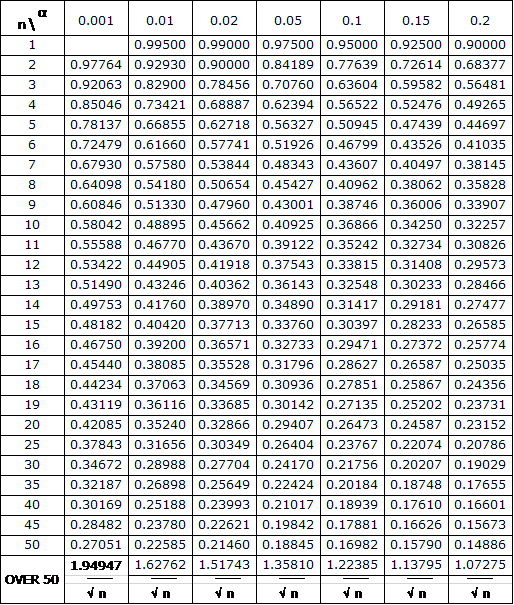
\includegraphics[height=0.5\textheight, angle=0]{"pdf/tablicaK.png"}
\end{center} \end{figure}

\newpage
\section{Dane}

\begin{center}
\tiny
\csvreader[tabular = |c|c|,
table head = \hline \bfseries{Lp} & \bfseries{x} \\ \hline,
late after last line = \\ \hline]{w10zad13LaTex.csv}{}{\csvlinetotablerow}
\end{center}

\newpage
\begin{center}
\tiny
\csvreader[tabular = |c|c|,
table head = \hline \bfseries{Lp} & \bfseries{x} \\ \hline,
late after last line = \\ \hline]{w10zad13_TRLaTex.csv}{}{\csvlinetotablerow}
\end{center}

\newpage
% Laboratoria 12
\part{Laboratoria 12}
Celem tych laboratoriów było zapoznanie się z metodami analizy regresji i korelacji. Uzyskaliśmy wiedze o wyznaczaniu prostej regresji dla danych oraz sprawdzenie czy dwa zestawy danych są skorelowane dodatnio lub ujemnie oraz w jakim stopniu. Nauczyliśmy się także wyznaczać błędy zastosowanego modelu.

% Zadanie 1
\section{Zadanie 1}

Sporządzić diagram rozrzutu, wyznaczyć oceny współczynników korelacji i determinacji, wyznaczyć równania prostych regresji ($Y$ względem $X$, $X$ względem $Y$), błędy standardowe estymacji oraz wykreślić równanie regresji dla podanych prób:

\begin{enumerate}[label = \alph*)]

\item $[x; y] = $\\
$\{[5.5, 1.5], [8.5, 4.0], [4.0, 2.0], [8.0, 7.5], [2.5, 0.5], [8.0, 5.0], [8.5, 8.5], [3.5, 1.0], $\\
$[6.5, 2.5], [9.0, 8.0], [0.5, 1.0], [8.5, 6.5], [7.5, 3.5], [1.5, 1.0], [8.5, 9.5], $\\
$[2.0, 1.5], [8.0, 9.0], [7.5, 5.5], [9.0, 5.5], [7.0, 1.5], [7.5, 7.0], [5.0, 0.5], $\\
$[4.5, 1.5], [5.5, 2.5], [6.5, 4.0]\}$.

\item $[x; y] = $\\
$\{[3.4, 3.7], [2.7, 4.7], [4.4, 4.6], [2.6, 2.5], [5.2, 5.3], [3.1, 4.6], [2.2, 3.5], [3.3, 4.1], $\\
$[6.0, 5.3], [4.0, 5.4], [2.0, 2.7], [3.9, 5.0], [2.5, 1.5], [2.5, 4.3], [3.6, 3.0], [6.4, 5.1], $\\
$[2.8, 3.7], [4.3, 5.8], [5.7, 5.5], [2.5, 3.2], [4.9, 5.0], [3.0, 1.8], [3.6, 4.3], [5.7,4.9], $\\
$[3.0, 1.0], [4.1, 4.1], [5.0, 4.8], [2.2, 2.0], [3.7, 3.4], [5.0, 5.7], [3.1, 4.4], [3.4,5.4], $\\
$[3.4, 2.3], [2.5, 2.9], [5.3, 5.0], [4.1,4.6], [3.0, 5.0], [2.8, 2.3], [3.0, 3.9], [2.4, 3.9], $\\
$[4.5, 5.5], [3.5, 5.0], [4.8, 5.3], [3.1, 2.5], [2.7, 4.1], [3.0, 3.3], [4.2, 5.0], [3.3, 2.2], $\\
$[3.6, 3.9], [3.4, 4.7]\}$.
\end{enumerate}

\subsection{Diagram rozrzutu}
Jako pierwsze sporządzono diagram rozrzutu gdzie na osi X są wartości $x$, a na osi Y wartości $y$. Wykres sporządzono w R.
\begin{figure}[h!]
\begin{center}
\includegraphics[height = 0.4\textheight, angle = 0]{"w11zad1a.png"}
\end{center} \end{figure} 

\newpage
\begin{figure}[h!]
\begin{center}
\includegraphics[height = 0.4\textheight, angle = 0]{"w11zad1b.png"}
\end{center} \end{figure} 

\subsection{Współczynnik korelacji}
Obliczymy teraz współczynnik korelacji zgodnie ze wzorem:
\[ r = \frac{SS_{xy}}{\sqrt{SS_{xx} \cdot SS_{yy}}} \]
Gdzie:
\[ SS_{xx} = \sum (x_i^2) - \frac{(\sum x_i )^2}{n} \overset{R}{=} sum(x^2) - sum(x)^2/length(x) \]
\[ SS_{xy} = \sum x_i y_i - \frac{\sum x_i \cdot \sum y_i}{n} \overset{R}{=} sum(x*y) - sum(x)*sum(y)/length(x) \]

Otrzymano następujące wartości:
\begin{center} \begin{tabular}{|c|c|c|c|c|} \hline
 & $SS_{xx}$ & $SS_{yy}$ & $SS_{xy}$ & r \\ \hline
a) & 155.64 & 209.74 & 142.44 & 0.7883711 \\ \hline
b) & 57.4248 & 74.1122 & 42.3684 & 0.6494526 \\ \hline
\end{tabular} \end{center}

Ponieważ oba $r$ są dodatnie możemy sformułować hipotezę że współczynnik korelacji pomiędzy $x$ i $y$ jest dodatni.
\begin{center} \begin{tabular}{|c|c|} \hline
$H_0$ & $\rho \leq 0$ \\ \hline
$H_1$ & $\rho > 0$ \\ \hline
\end{tabular} \end{center}

Aby sprawdzić tę hipotezę zastosujemy następującą statystykę:
\[ Z = (U - u_0) \cdot \sqrt{n-3} \]
Która, dla $n > 7$ ma w przybliżeniu standardowy rozkład normalny. Poniżej przedstawiono obliczenia dla: \\ \par
a)
\[U = \frac{1}{2} \ln \frac{1+r}{1-r} = \frac{1}{2} \ln(\frac{1.7883711}{0.2116289} \approx 1.067113 \]
\[ u_0 = \frac{1}{2} \ln \frac{1+\rho_0}{1-\rho_0} + \frac{\rho_0}{2n-2} = 0 \]
\[ Z_0 = 2.51587 \cdot \sqrt{10 -3} \approx 5.005205 \]

b)
\[U = \frac{1}{2} \ln \frac{1+r}{1-r} = \frac{1}{2} \ln(\frac{1.6494526}{0.3505474} \approx 0.7743514 \]
\[ u_0 = \frac{1}{2} \ln \frac{1+\rho_0}{1-\rho_0} + \frac{\rho_0}{2n-2} = 0 \]
\[ Z_0 = 2.51587 \cdot \sqrt{10 -3} \approx 5.308686 \]

Wtedy można obliczyć \textit{p-value} dla oby prób, zgodnie ze wzorem:
\begin{align*} \text{p-value}_a & = 1 - \Phi(5.005205) \overset{R}{=} 1 - pnorm(5.005205, 0, 1) \approx 2.790134e-07 \\
\text{p-value}_b & = 1 - \Phi(5.308686) \overset{R}{=} 1 - pnorm(5.308686, 0, 1) \approx 5.520921e-08 \end{align*}

Przyjmując $\alpha = 0.05$ oba \textit{p-value} są mniejsze od $\alpha$; zatem odrzucamy hipotezę zerową i wnioskujemy że korelacja pomiędzy $x$ i $y$ jest typu dodatniego, co widać na wykresach i z obliczonych wartości $r$. \\ \par

\subsection{Współczynnik determinacji i równania regresji}
Aby wyznaczyć współczynnik determinacji potrzebne jest wyliczenie SSE, które wyraża się następująco:
\[ \text{SSE} = \sum (y_i - \text{\^y}_i)^2 \]
lub
\[ \text{SSE} = \sum (x_i - \text{\^x}_i)^2 \]

Zatem potrzebujemy najpierw wyznaczyć równanie regresji. Do tego równania potrzebujemy dwa współczynniki:
\[ \beta_0 = \overline{y} - \beta_1 \overline{x} \overset{R}{=} mean(y) - b1*mean(x) \]
\[ \beta_1 = \frac{SS_{xy}}{SS_{xx}} = b1\]
Natomiast dla $X$ zależne od $Y$ parametry są następujące:
\[ \beta_0 = \overline{x} - \beta_1 \overline{y} \overset{R}{=} mean(x) - b1*mean(y) \]
\[ \beta_1 = \frac{SS_{xy}}{SS_{yy}} = b1\]

Rozważymy najpierw $Y$ zależne od $X$. Równania wyglądają następująco:
\begin{align*}
y & = \beta_0 + \beta_1 \cdot x \\
y_a & = -1.580956  +  0.9151889 \cdot x \\
y_b & = 1.342481  +  0.7378067 \cdot x
\end{align*}

Wtedy parametry SSE wynoszą:
\begin{center} \begin{tabular}{|c|c|} \hline
& SSE \\ \hline
a) & 79.38049 \\ \hline
b) & 42.85251 \\ \hline
\end{tabular} \end{center}

Możemy teraz wyznaczyć współczynnik determinacji, który wynosi:
\[ r^2 = 1 - \frac{SSE}{SS_{yy}} \]
\begin{center} \begin{tabular}{|c|c|} \hline
& $r^2$ \\ \hline
a) & 0.6215291 \\ \hline
b) & 0.4217887 \\ \hline
\end{tabular} \end{center}

Następnie rozważymy dla $X$ zależnego od $Y$. Wtedy, analogicznie do wcześniej:
\begin{align*}
x & = \beta_0 + \beta_1 \cdot y \\
x_a & = 3.389911  +  0.6791265 \cdot y \\
x_b & = 1.341846  +  0.5716792 \cdot y
\end{align*}

Wtedy parametry SSE wynoszą:
\begin{center} \begin{tabular}{|c|c|} \hline
& SSE \\ \hline
a) & 58.90522 \\ \hline
b) & 33.20367 \\ \hline
\end{tabular} \end{center}

Możemy teraz wyznaczyć współczynnik determinacji, który wynosi:
\[ r^2 = 1 - \frac{SSE}{SS_{yy}} \]
\begin{center} \begin{tabular}{|c|c|} \hline
& $r^2$ \\ \hline
a) & 0.6215291 \\ \hline
b) & 0.4217887 \\ \hline
\end{tabular} \end{center}

Wartości $r^2$ nie zmieniają się, zatem, równanie regresji zmniejsza całkowitą sumę kwadratów o 62\% dla próby a) i 42\% dla próby b) od średniej arytmetycznej.

\subsection{Błąd modelu}
Następnie obliczymy błędy modelu zgodnie ze wzorem:
\[ S^2 = \frac{SSE}{n-2} \]
Liczebności prób są, dla a) $n = 25$, dla b) $n = 50$. Wtedy błędy modelu są następujące:
\begin{center} \begin{tabular}{|c|c|c|} \hline
& Y od X & X od Y \\ \hline
a) & 3.451326 & 2.561096 \\ \hline
b) & 0.8927607 & 0.6917431 \\ \hline
\end{tabular} \end{center}

\subsection{Wykresy regresji}
Jako ostatnie przedstawiono wykresy prostych regresji na wykresach z danymi.
\begin{figure}[h!]
\begin{center}
\includegraphics[height = 0.5\textheight, angle = 0]{"w11zad1a_r.png"}
\end{center} \end{figure} 

\newpage
\begin{figure}[h!]
\begin{center}
\includegraphics[height = 0.5\textheight, angle = 0]{"w11zad1b_r.png"}
\end{center} \end{figure} 

Dla danych a) prosta x(y) lepiej obrazuje przebieg danych, natomiast dla danych b) nie ma znacznej różnicy pomiędzy prostymi.

\newpage
% Zadanie 2
\section{Zadanie 2}

Odnotowano miesięczne dochody przypadające na jednego członka rodziny (w zł) - cecha $X$ oraz wyrażoną w procentach część budżetu rodzinnego przeznaczoną na zakup artykułów żywnościowych i utrzymanie mieszkania - cecha $Y$.
\begin{center} \begin{tabular}{|c|c|c|c|c|c|c|c|c|c|c|} \hline
X & 200 & 300 & 150 & 225 & 175 & 350 & 150 & 250 & 325 & 250 \\ \hline
Y & 70 & 80 & 95 & 75 & 90 & 60 & 60 & 65 & 85 & 90 \\ \hline
\end{tabular} \end{center}
Sporządzić diagram rozrzutu, wyznaczyć oceny współczynników korelacji i determinacji między dochodem przypadającym na jednego członka rodziny a wydatkami na artykuły żywnościowe i utrzymanie mieszkania. \\ \par

Wykres sporządzono w R wygląda następująco:
\begin{figure}[h!]
\begin{center}
\includegraphics[height = 0.5\textheight, angle = 0]{"w11zad2.png"}
\end{center} \end{figure} 

Obliczymy teraz współczynnik korelacji zgodnie ze wzorem:
\[ r = \frac{SS_{xy}}{\sqrt{SS_{xx} \cdot SS_{yy}}} \]
Gdzie:
\[ SS_{xx} = \sum (x_i^2) - \frac{(\sum x_i )^2}{n} \overset{R}{=} sum(x^2) - sum(x)^2/length(x) \]
\[ SS_{xy} = \sum x_i y_i - \frac{\sum x_i \cdot \sum y_i}{n} \overset{R}{=} sum(x*y) - sum(x)*sum(y)/length(x) \]

Otrzymano następujące wartości:
\begin{center} \begin{tabular}{|c|c|c|c|} \hline
$SS_{xx}$ & $SS_{yy}$ & $SS_{xy}$ & r \\ \hline
45312.5 & 1510 & -1625 & -0.1964517 \\ \hline
\end{tabular} \end{center}

Aby sprawdzić ten współczynnik to wyznaczymy hipotezę zerową orzekającą, że istnieje dodatnia korelacja:
\begin{center} \begin{tabular}{|c|c|} \hline
$H_0$ & $\rho \geq 0$ \\ \hline
$H_1$ & $\rho < 0$ \\ \hline
\end{tabular} \end{center}

Skorzystamy ze statystki testowej:
\[ Z = (U - u_0) \cdot \sqrt{n-3} \]
Która ma w przybliżeniu standardowy rozkład normalny.

\[U = \frac{1}{2} \ln \frac{1+r}{1-r} = \frac{1}{2} \ln(\frac{0.8035483}{1.1964517} \approx -0.199039 \]
\[ u_0 = \frac{1}{2} \ln \frac{1+\rho_0}{1-\rho_0} + \frac{\rho_0}{2n-2} = 0 \]
\[ Z_0 = -0.199039 \cdot \sqrt{10 -3} \approx -0.526608 \]

Obliczymy teraz \textit{p-value} która wynosi:
\[ \text{p-value} = \Phi(-0.526608) \overset{R}{=} pnorm(-0.526608, 0, 1) \approx 0.2992329 \]

Wartość ta jest większa niż większość standardowo przyjętych $\alpha$ zatem nie możemy odrzucić hipotezę zerową więc nie istnieje ujemna korelacja między cechą $X$ i $Y$.

Aby wyznaczyć współczynnik determinacji potrzebne jest wyliczenie SSE, które wyraża się następująco:
\[ \text{SSE} = \sum (y_i - \text{\^y}_i)^2 \]
Zatem potrzebujemy najpierw wyznaczyć równanie regresji. Do tego równania potrzebujemy dwa współczynniki:
\[ \beta_0 = \overline{y} - \beta_1 \overline{x} \overset{R}{=} mean(y) - b1*mean(x) \approx 85.51724\]
\[ \beta_1 = \frac{SS_{xy}}{SS_{xx}} = b1 \approx -0.03586207\]
Wtedy podstawiając kolejne wartosci $x_i$ do równania regresji możemy obliczyć SSE:
\[ \text{\^y}_i = \beta_0 + \beta_1 \cdot x_i = 85.51724 - 0.03586207 \cdot x_i \]

Wtedy $SSE = 1451.724$ i można obliczyć współczynnik determinacji:
\[ r^2 = 1 - \frac{SSE}{SS_{yy}} = 1 - \frac{1451.724}{1510} \approx 0.03859329 \]

Zatem równanie regresji zmniejsza całkowitą sumę kwadratów próby o 3\% od średniej arytmetycznej.

\newpage
% Zadanie 3
\section{Zadanie 3}
Naturalne jest przekonanie, że powinna być silna korelacja pomiędzy miesięcznymi obrotami firmy a jej liczebnością personelu handlowego. Dla pewnej firmy zostały zebrane dane dotyczące liczby sprzedawców w ostatnich 10 kwartałach oraz osiągane średniomiesięczne obroty (w mln zł) w tym czasie. \\
Wynoszą one: [15, 1.35], [18, 1.63], [24, 2.33], [22, 2.41], [25, 2.63], [29, 2.93], [30, 3.41], [32, 3.26], [35, 3.63], [38, 4.15].\\
Sprawdzić, czy to przekonanie potwierdziło się dla badanej firmy. \\ \par

Sporządzono wykres rozrzutu w celu wstępnego sprawdzenia danych; wykres przygotowany w R.
\begin{figure}[h!]
\begin{center}
\includegraphics[height = 0.5\textheight, angle = 0]{"w11zad3.png"}
\end{center} \end{figure} 

Z wykresu widać że może istnieć dodatnia korelacja pomiędzy danymi. $x$ oznacza liczbę pracowników, natomiast $y$ oznacza średnio-miesięczne obroty. \\
Następnie został obliczony współczynnik korelacji zgodnie ze wzorami podanymi w poprzednim zadaniu. Uzyskano następujące wartości:
\begin{center} \begin{tabular}{|c|c|c|c|} \hline
$SS_{xx}$ & $SS_{yy}$ & $SS_{xy}$ & r \\ \hline
485.6 & 6.97801 & 57.456 & 0.9870298 \\ \hline
\end{tabular} \end{center}

Wartość ta jest dodatnia, zatem jest możliwe że korelacja jest typu dodatniego. W celu sprawdzenia tego sporządzona została teza alternatywna i zerowa wyznaczona poniżej. $\rho$ jest rzeczywistym współczynnikiem korelacji.
\begin{center} \begin{tabular}{|c|c|} \hline
$H_0$ & $\rho \leq 0$ \\ \hline
$H_1$ & $\rho > 0$ \\ \hline
\end{tabular} \end{center}

Ponieważ liczba obserwacji $n = 10 > 7$ możemy zastosować statystykę jak w poprzednim zadaniu.
\[ Z = (U - u_0) \cdot \sqrt{n-3} \]

\[U = \frac{1}{2} \ln \frac{1+r}{1-r} = \frac{1}{2} \ln(\frac{1.9870298}{0.0129702} \approx 2.51587 \]
\[ u_0 = \frac{1}{2} \ln \frac{1+\rho_0}{1-\rho_0} + \frac{\rho_0}{2n-2} = 0 \]
\[ Z_0 = 2.51587 \cdot \sqrt{10 -3} \approx 6.656366 \]

Obliczymy teraz \textit{p-value} zgodnie ze wzorem:
\[ \text{p-value} = 1 - \Phi(6.656366) \overset{R}{=} 1 - pnorm(6.656366, 0, 1) \approx 1.4034e-11 \]

Przyjmując $\alpha = 0.05$ widzimy że \textit{p-value} jest od tej wartości mniejsze; zatem możemy odrzucić hipotezę zerową i wnioskować że istnieje dodatnia korelacja między liczbą personelu i miesięcznymi obrotami.

\newpage
% Laboratoria 13
\part{Laboratoria 13}
Celem tych laboratoriów było zapoznanie się z metodami analizy wariancji czyli testów ANOVA dla zależności od jednego parametru dla danych normalnych i w postaci blokowej. Testy tego typu zostały przeprowadzone za pomocą programów komputerowych, zatem uzyskaliśmy wiedzę jak te testy przeprowadzać ze wspomaganiem oraz jak dane przygotować żeby program mógł je prawidłowo odczytać.

% Zadanie 1
\section{Zadanie 1}
(Krysicki 5.2). Zmierzono długości czasów świecenia trzech typów żarówek, otrzymując (w h):
\begin{enumerate}[label = dla typu \arabic*:]
\item 1802, 1992, 1854, 1880, 1761, 1900;
\item 1664, 1755, 1823, 1862;
\item 1877, 1710, 1882, 1720, 1950.
\end{enumerate}
Na poziomie istotności $\alpha=0,05$ zweryfikować hipotezę, że wartości przeciętne czasów świecenia żarówek tych typów są jednakowe. \\ \par

Dane przygotowano w postaci pliku csv w celu obliczenia testu ANOVA w R.
\begin{center}
\csvreader[tabular = |c|c|,
table head = \hline \bfseries{data} & \bfseries{type} \\ \hline,
late after last line = \\ \hline]{w12zad1.csv}{}{\csvlinetotablerow}
\end{center}

Dane te wgrano w R w następujący sposób: \textit{data = read.csv("w12zad1.csv", colClasses = c("numeric", "factor")}. \\
Obliczenie testu ANOVA w R przeprowadzono w następujący sposób: \\
\textit{model = aov(data$\sim$type, data)} \\
\textit{summary(model)} \\
Otrzymano następujący tablicowy wynik:

\begin{center} \begin{tabular}{|c|c|c|c|c|c|} \hline
& Df & Sum Sq & Mean Sq & F value & Pr($>$F) \\ \hline
type & 2 & 18947 & 9473 & 1.127 & 0.356 \\ \hline
Residuals & 12 & 100864 & 8405 & & \\ \hline
\end{tabular} \end{center}

Funkcja oblicza \textit{p-value} zapisane w ostatniej kolumnie, które jest większe od przyjętego poziomu istotności $\alpha=0.05$. Zatem nie mamy podstaw aby odrzucić hipotezę zerowa o równaniu się wartości przeciętnych czasów świecenia żarówek.

\newpage
% Zadanie 2
\section{Zadane 2}
(Krysicki 5.3). Spośród trzech odmian ziemniaków każdą uprawiano na 12 działkach tej samej wielkości i rodzaju. Działki te podzielono na 4 grupy po 3 działki i dla każdej grupy zastosowano różny rodzaj nawozu. Plony w $q$ zestawione w tabeli:
\begin{center} \begin{tabular}{|c|ccc|ccc|ccc|ccc|} \hline
Odmiana & \multicolumn{12}{|c|}{Nawóz} \\ \cline{2-13}
& \multicolumn{3}{|c|}{1} & \multicolumn{3}{|c|}{2} & \multicolumn{3}{|c|}{3} & \multicolumn{3}{|c|}{4} \\ \hline
1 & 5,6 & 6,1 & 5,9 & 6,6 & 6,7 & 6,6 & 7,7 & 7,3 & 7,4 & 6,3 & 6,4 & 6,3 \\ 
2 & 5,7 & 4,9 & 5,1 & 6,5 & 6,7 & 6,6 & 6,9 & 7,1 & 6,5 & 6,6 & 6,7 & 6,7 \\ 
3 & 6,3 & 6,1 & 6,3 & 6,5 & 6,4 & 6,2 & 6,6 & 6,6 & 6,8 & 6,3 & 6,1 & 6,0 \\ \hline
\end{tabular} \end{center}

Na poziomie istotności $\alpha=0,05$ zweryfikować następujące hipotezy:
\begin{enumerate}[label = \alph*)]
\item wartości przeciętne plonów dla różnych odmian nie różnią się istotnie niezależnie od stosowanego nawozu,
\item wartości przeciętne plonów dla różnych nawozów nie różnią się istotnie niezależnie od odmiany,
\item interakcja między odmianami i nawozami jest równa 0.
\end{enumerate}

Dane przygotowano w postaci pliku csv w celu obliczenia testu ANOVA w R.
\begin{center}
\scriptsize
\csvreader[tabular = |c|c|c|,
table head = \hline \bfseries{data} & \bfseries{odmiana} & \bfseries{nawoz} \\ \hline,
late after last line = \\ \hline]{w12zad2.csv}{}{\csvlinetotablerow}
\end{center}

\subsection{a)}
Dane te wgrano w R w następujący sposób: \textit{data = read.csv("w12zad2.csv", colClasses = c("numeric", "factor", "factor")}. \\
Obliczenie testu ANOVA w R przeprowadzono w następujący sposób: \\
\textit{model = aov(data$\sim$odmiana + nawoz, data)} \\
\textit{summary(model)} \\
Otrzymano następujący tablicowy wynik:

\begin{center} \begin{tabular}{|c|c|c|c|c|c|} \hline
& Df & Sum Sq & Mean Sq & F value & Pr($>$F) \\ \hline
odmiana & 2 & 4.101 & 2.0503 & 16.900 & 1.21e-05 \\ \hline
nawoz & 3 & 3.116 & 1.0388 & 8.563 & 0.000294 \\ \hline
Residuals & 30 & 3.639 & 0.1213 & & \\ \hline
\end{tabular} \end{center}

Funkcja oblicza \textit{p-value} w ostatniej kolumnie. Dla typu nawozu widzimy że wartość 0.000294 jest mniejsza od przyjętego poziomu istotności $\alpha = 0.05$, zatem wartości przeciętne plonów różnią się istotnie zależnie od stosowanego nawozu.

\subsection{b)}
Korzystając z tabeli poprzedniego podpunktu widzimy że \textit{p-value =  1.12e-05} dla typu odmiany jest mniejsze od przyjętego poziomu istotności $\alpha = 0.05$. Zatem wartości przeciętne plonów dla rożnych nawozów różnią się istotnie zależnie od odmiany.

\subsection{c)}
Aby sprawdzić interakcje między nawozami i odmianami możemy zastosować test Tukeya w R następująco: \textit{TukeyHSD(model, conf.level = 0.95)}. Funkcja ta oddaje następujące tablice:

\begin{center} \begin{tabular}{|c|c|c|c|c|} \hline
\multicolumn{5}{|c|}{\$odmiana} \\ \hline
& diff & lwr & upr & p adj \\ \hline
2-1 & 0.8250000 & 0.4744532 & 1.17554680 & 0.0000071 \\ \hline
3-1 & 0.4583333 & 0.1077865 & 0.80888014 & 0.0083242 \\ \hline
3-2 & -0.3666667 & -0.7172135 & -0.01611986 & 0.0388934 \\ \hline
\multicolumn{5}{|c|}{\$nawoz} \\ \hline
2-1 & -0.4000000 & -0.84645464 & 0.04645464 & 0.0917316 \\ \hline
3-1 & 0.4111111 & -0.03534353 & 0.85756575 & 0.0796887 \\ \hline
4-1 & 0.1555556 & -0.29089908 & 0.60201019 & 0.7797038 \\ \hline
3-2 & 0.8111111 & 0.36465647 & 1.25756575 & 0.0001551 \\ \hline
4-2 & 0.5555556 & 0.10910092 & 1.00201019 & 0.0102547 \\ \hline
4-3 & -0.2555556 & -0.70201019 & 0.19089908 & 0.4179349 \\ \hline
\end{tabular} \end{center}

Obliczone są \textit{p-value} zatem możemy dokonać wnioski. Dla różnicy odmian widzimy że wszystkie \textit{p-value} są mniejsze od $\alpha = 0.05$, zatem każda wartość przeciętna dla odmian różni się, więc różnice nie są równe 0. \\
Dla nawozów natomiast istnieją wartości \textit{p-value} większe od $\alpha = 0.05$ są to różnice: 1-3, 1-4, 3-4. Oznacza to że dla tych nawozów różnica wartości przeciętnych jest z dużym prawdopodobieństwem 0. Natomiast dla reszty nawozów różnice nie są równe 0 bo przeciętne wartości różnią się za dużo.

\newpage
% Zadanie 3
\section{Zadanie 3}
Rozwiązać zadanie 5.7 z Krysickiego. \\ \par

Z trzech różnych wydziałów pewnej uczelni wylosowano po pięciu studentów z każdego roku studiów i obliczono średnią ocen uzyskaną przez każdego studenta w ostatnim semestrze. Uzyskano rezultaty
\begin{center} \begin{tabular}{|c|cccc|cccc|cccc|} \hline
Rok & \multicolumn{12}{|c|}{Wydział} \\ \cline{2-13}
studiów & \multicolumn{4}{|c|}{A} & \multicolumn{4}{|c|}{B} & \multicolumn{4}{|c|}{C} \\ \hline
I & 2.6 & 4.1 & 3.1 & 2.4 & 3.1 & 2.5 & 3.3 & 3.8 & 2.7 & 4.2 & 2.9 & 3.7 \\ 
II & 2.8 & 4.3 & 3.8 & 3.0 & 3.9 & 2.6 & 3.2 & 3.3 & 3.0 & 4.4 & 3.9 & 3.1 \\ 
III & 3.2 & 4.1 & 4.8 & 4.0 & 3.4 & 2.9 & 4.1 & 2.8 & 4.0 & 3.3 & 3.4 & 3.0 \\ 
IV & 3.2 & 3.9 & 4.2 & 3.6 & 3.6 & 4.4 & 2.8 & 3.9 & 3.7 & 5.0 & 2.6 & 3.4 \\ 
V & 4.0 & 4.0 & 3.5 & 3.8 & 4.0 & 3.0 & 4.5 & 3.7 & 3.0 & 3.8 & 4.8 & 3.5 \\ \hline
\end{tabular} \end{center}

Zakładając, że średnie uzyskiwanych ocen mają rozkłady normalne o tej samej wariancji na poziomie $\alpha = 0.05$, zweryfikować następujące hipotezy:
\begin{enumerate}[label = \alph*)]
\item wartości przeciętne średnich ocen dla studentów różnych wydziałów są jednakowe;
\item wartości przeciętne średnich ocen dla różnych lat studiów są jednakowe;
\item wartości przeciętne ocen średnich dla pierwszych dwóch lat są jednakowe;
\end{enumerate}

Wartości z tabeli przepisano do pliku csv w celu wgrania go do programu R. 
\begin{center}
\scriptsize
\csvreader[tabular = |c|c|c|,
table head = \hline \bfseries{data} & \bfseries{wydzial} & \bfseries{rok} \\ \hline,
late after last line = \\ \hline]{w12zad3.csv}{}{\csvlinetotablerow}
\end{center}

\subsection{a)}
Dane z pliku csv wgrano pod zmienną "data" w następujący sposób: \textit{data = read.csv("w12zad3.csv", colClasses = c("numeric", "factor", "factor")}. \\
Test ANOVA natomiast wykonano w następujący sposób: \textit{model = aov(data$\sim$wydzial, data)}. Otrzymano następujący wynik \textit{summary(model)} =
\begin{center} \begin{tabular}{|c|c|c|c|c|c|} \hline
& Df & Sum Sq & Mean Sq & F value & Pr($>$F) \\ \hline
wydzial & 2 & 0.345 & 0.1727 & 0.437 & 0.648 \\ \hline
Residuals & 57 & 22.502 & 0.3948 & & \\ \hline
\end{tabular} \end{center}

Ponieważ \textit{p-value}, obliczone w ostatniej kolumnie, jest większe niż $\alpha = 0.05$ wnioskujemy że wartości przeciętne średnich ocen dla studentów różnych wydziałów są sobie równe.

\subsection{b)}
Test ANOVA przeprowadzono podobnie jak w poprzednim podpunkcie, tj: \textit{model = aov(data$\sim$rok, data)}. Otrzymano następujące wyniki \textit{summary(model)} =
\begin{center} \begin{tabular}{|c|c|c|c|c|c|} \hline
& Df & Sum Sq & Mean Sq & F value & Pr($>$F) \\ \hline
rok & 4 & 2.612 & 0.6531 & 1.775 & 0.147 \\ \hline
Residuals & 55 & 20.235 & 0.3679 & & \\ \hline
\end{tabular} \end{center}

Ponieważ \textit{p-value}, obliczone w ostatniej kolumnie, jest większe niż $\alpha = 0.05$ wnioskujemy że wartości przeciętne średnich ocen dla studentów różnych lat studiów są sobie równe.

\subsection{c)}
Ponieważ zakładamy że dane mają rozkład normalny możemy zastosować test Tukeya w następujący sposób: \textit{tukey = TukeyHSD(model, conf.level = 0.95)}
Otrzymano następujący wynik
\begin{center} \begin{tabular}{|c|c|c|c|c|} \hline
& diff & lwr & upr & p adj \\ \hline
II-I & 0.2416667 & -0.45671717 & 0.9400505 & 0.8648729 \\ \hline
III-I & 0.3833333 & -0.31505051 & 1.0817172 & 0.5364514 \\ \hline
IV-I & 0.4916667 & -0.20671717 & 1.1900505 & 0.2865813 \\ \hline
V-I & 0.6000000 & -0.09838384 & 1.2983838 & 0.1244862 \\ \hline
III-II & 0.1416667 & -0.55671717 & 0.8400505 & 0.9785925 \\ \hline
IV-II & 0.2500000 & -0.44838384 & 0.9483838 & 0.8498736 \\ \hline
V-II & 0.3583333 & -0.34005051 & 1.0567172 & 0.6004999 \\ \hline
IV-III & 0.1083333 & -0.59005051 & 0.8067172 & 0.9921775 \\ \hline
V-III & 0.2166667 & -0.48171717 & 0.9150505 & 0.9048593 \\ \hline
V-IV & 0.1083333 & -0.59005051 & 0.8067172  & 0.9921775 \\ \hline
\end{tabular} \end{center}

Dla tego typu testu dostajemy także \textit{p-value} i widzimy że każda ta wartość jest większa od $\alpha = 0.05$. Zatem wnioskujemy że wartości średnie dla pierwszych dwóch lat są jednakowe.

\newpage
% Zadanie 4
\section{Zadanie 4}
Korzystając ze wspomagania komputerowego rozwiązać przykład 3 z wykładu. \\ \par

Jednym z aspektów jakości samochodów osobowych jest koszt naprawy uszkodzeń spowodowanych drobnymi ulicznymi stłuczkami. Decydujące znaczenie mają tu zderzaki. Producent rozważa wprowadzenie nowego typu
zderzaków spośród czterech zaprojektowanych typów. Zainstalowano po siedem zderzaków każdego typu na pojazdach
popularnej klasy i poddano je próbom zderzania ze ścianą
z prędkością 30 km/h. Następnie oszacowano koszty napraw
powstałych uszkodzeń (w j.m.). Wyniki są przedstawione w
tablicy.

\begin{center} \begin{tabular}{|c|c|c|c|} \hline
\multicolumn{4}{|c|}{Typ zderzaka} \\ \hline
1 & 2 & 3 & 4 \\ \hline
315 & 285 & 269 & 255 \\ \hline
288 & 292 & 277 & 287 \\ \hline
293 & 263 & 273 & 265 \\ \hline
306 & 249 & 252 & 279 \\ \hline
299 & 275 & 263 & 241 \\ \hline
310 & 266 & 251 & 312 \\ \hline
282 & 252 & 272 & 310 \\ \hline
\end{tabular} \end{center}

\begin{enumerate}[label = \alph*)]
\item Przyjmując 5-procentowy poziom istotności zbadać, czy są
istotne różnice w kosztach usuwania uszkodzeń dla badanych
czterech typów zderzaków.
\item W przypadku występowania różnic ustalić typy zderzaków
różniących się ze względu na koszty usuwania awarii.
\end{enumerate}

\subsection{a)}
Wartości z tablicy wybrano do pliku csv aby wczytać je w R. Wartości zapisano w kolumnie nazwaną "data" a odpowiadające wartościom typy zderzaka zapisano pod kolumną "type" i uwzględniono w R że to ma być kolumna typu "factor". Dane wgrano korzystając z funkcji \textit{data = read.csv("w12zad4.csv")}. \\
Aby sprawdzić czy są istotne różnice w kosztach usuwania uszkodzeń wykorzystano następującą funkcje: \textit{model = aov(data$\sim$type, data=data)} która wykonuje test ANOVA jedno kierunkowy na zależność kosztu od typu zderzaka. Poniżej uzyskane tą funkcją wyniki (\textit{summary(model)}).
\begin{center} \begin{tabular}{|c|c|c|c|c|c|} \hline
& Df & Sum Sq & Mean Sq & F value & Pr($>$F) \\ \hline
type & 3 & 4805 & 1601.6 & 5.197 & 0.00658  \\ \hline
Residuals & 24 & 7396 & 308.2 & \multicolumn{2}{|c|}{} \\ \hline
\end{tabular} \end{center}

Funkcja ta oddaje \textit{p-value} zapisane pod ostatnią kolumną, zatem, przyjmując $\alpha = 0.05$ stwierdzamy że typ zderzaka ma wpływ na koszt usuwania uszkodzeń.

\subsection{b)}
Ponieważ w podpunkcie \textbf{a)} okazało się że występują różnice w kosztach usuwania uszkodzeń więc możemy poszukać które typy różnią się od siebie. W R istnieje funkcja obliczająca test Tukeya na podstawie wcześniej wyznaczonej analizy wariancji (\textit{aov()}). Ten test został wywołany następująco: \textit{TukeyHSD(model, conf.level = 0.95)}. \\
Otrzymano następującą tabele:
\begin{center} \begin{tabular}{|c|c|c|c|c|} \hline
& diff & lwr & upr & p adj \\ \hline
2-1 & -30.142857 & -56.02790 & -4.257812 & 0.0182410 \\ \hline
3-1 & -33.714286 & -59.59933 & -7.829241 & 0.0074533 \\ \hline
4-1 & -20.571429 & -46.45647 & 5.313616 & 0.1540625 \\ \hline
3-2 & -3.571429 & -29.45647 & 22.313616 & 0.9807839 \\ \hline
4-2 & 9.571429 & -16.31362 & 35.456474 & 0.7394841 \\ \hline
4-3 & 13.142857 & -12.74219 & 39.027902 & 0.5111022 \\ \hline
\end{tabular} \end{center}

Funkcja ta także zwraca \textit{p-value} zatem, porównując z $\alpha = 0.05$ widzimy że jedynie typ 2 i typ 1 się różnią a także typ 1 i typ 3. \\
Obliczenia programem potwierdzają wyniki obliczone w przykładzie z wykładu.

\newpage
% Zadanie 6
\section{Zadanie 6}
Korzystając ze wspomagania komputerowego rozwiązać przykład 6 z wykładu. \\ \par

Wycena prywatyzowanego przedsiębiorstwa państwowego poprzedzona jest szczegółową analizą wartości majątku, potencjału produkcyjnego, możliwości przestawienia produkcji, sposobów zabezpieczenia socjalnego pracowników, itp. Szacowanie wartości majątku przeprowadzają specjalistyczne firmy zajmujące się wyceną. Przeszacowanie wartości przedsiębiorstwa zmniejsza szanse prywatyzacji firmy, natomiast zaniżenie wartości zmniejsza przychód z prywatyzacji. \\

W celu zmniejszenia ryzyka popełnienia błędu przedstawiciel odpowiedniego ministerstwa zamierza porównać średnie oszacowania wartości trzech niezależnych firm wyceniających majątek zanim zleci jednej z nich dokonanie oszacowania wartości rynkowej prywatyzowanego przedsiębiorstwa. \\

Przedstawiciel zebrał informacje o wycenie majątku tych samych czterech przedsiębiorstw przez każdą z rozważanych trzech firm wyceniających. Uzyskane dane o wycenach (w mln zł) są podane w tabeli.

\begin{center} \begin{tabular}{|c|c|c|c|c|} \hline
Firma & \multicolumn{4}{|c|}{Wycena przedsiębiorstwa} \\ 
wyceniająca & 1 & 2 & 3 & 4 \\ \hline
A & 4.6 & 6.2 & 5.0 & 6.6 \\
B & 4.9 & 6.3 & 5.4 & 6.8 \\ 
C & 4.4 & 5.9 & 5.4 & 6.3 \\ \hline
\end{tabular} \end{center}

\begin{enumerate}[label = \alph*)]
\item Przeprowadzić analizę wariancji dla przeprowadzonych wycen. Na poziomie istotności $\alpha=0,05$ sprawdzić, czy są istotne różnice między oczekiwanymi wycenami dla zabiegów i bloków. 
\item Wyznaczyć 90-procentowy przedział ufności dla różnic między oczekiwanymi wycenami dla firm wyceniających A i B.
\end{enumerate}

Wartości z tabeli zapisano w pliku csv następującej postaci tak aby można było dokonać obliczenia w R.
\begin{center}
\csvreader[tabular = |c|c|c|,
table head = \hline \bfseries{data} & \bfseries{firma} & \bfseries{wycena} \\ \hline,
late after last line = \\ \hline]{w12zad6.csv}{}{\csvlinetotablerow}
\end{center}

\subsection{a)}
Jak w poprzednim zadaniu wykorzystamy funkcję R-owską \textit{model = aov(data$\sim$firma+wycena)}. Wynik tej funkcji można odczytać za pomocą \textit{summary(model)}.

\begin{center} \begin{tabular}{|c|c|c|c|c|c|c|} \hline
& Df & Sum Sq & Mean Sq & F value & Pr(>F) & \\ \hline
firma & 2 & 0.260 & 0.1300 & 4.179 & 0.073 & . \\ \hline
wycena & 3 & 6.763 & 2.2544 & 72.464 & 4.2e-05 & *** \\ \hline
Residuals & 6 & 0.187 & 0.0311 & & & \\ \hline
\end{tabular} \end{center}

\textit{Signif. codes:  0 '***' 0.001 '**' 0.01 '*' 0.05 '.' 0.1 ' ' 1} \\
Obliczone zostały przez funkcje \textit{p-value} zatem, porównując z $\alpha=0.05$ widzimy że nie ma różnicy wyceniania pomiędzy firmami, natomiast istnienie różnica wyceny między przedsiębiorstwami. Potwierdzone jest zatem to co zostało obliczone na wykładzie.

\subsection{b)}
Aby wyznaczyć przedział ufności wykorzystano funkcje \textit{TukeyHSD(model, conf.level = 0.9)} która oddaje następującą tablice:
\begin{center} \begin{tabular}{|c|c|c|c|c|} \hline
\multicolumn{5}{|c|}{\$firma} \\ \hline
& diff & lwr & upr & p adj \\ \hline
B-A & 0.25 & -0.06381888 & 0.56381888 & 0.1918699 \\ \hline
C-A & -0.10 & -0.41381888 & 0.21381888 & 0.7156978 \\ \hline
C-B & -0.35 & -0.66381888 & -0.03618112 & 0.0692699 \\ \hline
\multicolumn{5}{|c|}{\$wycena} \\ \hline
2-1 & 1.5000000 & 1.0860287 & 1.9139713 & 0.0001924 \\ \hline
3-1 & 0.6333333 & 0.2193620 & 1.0473047 & 0.0178616 \\ \hline
4-1 & 1.9333333 & 1.5193620 & 2.3473047 & 0.0000445 \\ \hline
3-2 & -0.8666667 & -1.2806380 & -0.4526953 & 0.0038512 \\ \hline
4-2 & 0.4333333 & 0.0193620 & 0.8473047 & 0.0851260 \\ \hline
4-3 & 1.3000000 & 0.8860287 & 1.7139713 & 0.0004312 \\ \hline
\end{tabular} \end{center}

Przedział ufności ma granice zaznaczone pod "lwr" i "upr". Zatem dla różnicy B-A przedział ufności jest następujący:
\[ (-0.06381888 ; 0.56381888 ) \]
Wynik ten nie zgadza się z wartościami obliczonymi na wykładzie, może to wynikać z tego że funkcja została źle użyta lub że wynik z wykładu jest nie prawidłowy.

\newpage
% Laboratoria 14
\part{Laboratoria 14}
Celem tych laboratoriów była kontynuacja pracy nad testami ANOVA. Wzbogaciliśmy zatem wiedzę w tej dziedzinie.

\begin{comment}
\section{Zadanie 1}
Pewna firma zakupiła dwie różne maszyny tłoczące uszczelki z arkuszy korka, gumy
lub plastiku. Firma chce poznać przeciętną liczbę uszczelek produkowanych przez te
maszyny na godzinę. W szczególności zainteresowanie dotyczy porównania wydajności
maszyn dla poszczególnych rodzajów uszczelek. W tym celu przeprowadzono
eksperyment $2 \times 3$ czynnikowy stosując trzy typy materiałów do produkcji uszczelek B1, B2 i B3 dla każdej maszyny tłoczącej uszczelki A1 i A2. Obydwie maszyny
pracowały przez trzy jednogodzinne okresy dla każdego z surowców z osiemnastoma
jednogodzinnymi okresami pracy związanymi z sześcioma kombinacjami maszyna-materiał w losowym porządku. \\
Celem randomizacji jest wyeliminowanie możliwych niekontrolowanych czynników
zewnętrznych mogących obciążać wyniki. \\
Dane do poszczególnych zabiegów wygenerować zgodnie z rozkładami normalnymi
\begin{center} \begin{tabular}{|c|c|c|} \hline
zabieg & i) & ii) \\ \hline
$A_1 B_1$ & N(16000; 2500) & N(16000; 2500) \\ \hline
$A_1 B_2$ & N(13000; 2500) & N(16000; 2500)\\ \hline
$A_1 B_3$ & N(15000; 2500) & N(17000; 2500) \\ \hline
$A_2 B_1$ & N(12000; 2500) & N(11000; 2500) \\ \hline
$A_2 B_2$ & N(9000; 2500) & N(13000; 2500) \\ \hline
$A_2 B_3$ & N(11000; 2500) & N(15000; 2500) \\ \hline
\end{tabular} \end{center}

\begin{enumerate}[label = \alph*)]
\item Sporządzić wykresy rozrzutu danych.
\item Zaznaczyć na wykresach średnie arytmetyczne z prób dla zabiegów.
\item Czy można z wykresu zauważyć interakcję maszyna-materiał?
\item Co można powiedzieć o wydajności badanych maszyn tłoczących?
\end{enumerate}
\end{comment}

\newpage
% Lab 14 - Zadanie 2
\section{Zadanie 2}
W celu sprawdzenia wpływu trzech typów maszyn M1, M2 i M3 na wydajność pracy
robotników, przeprowadzono eksperyment, w którym jako wydajność pracy mierzono
liczbę detali wyprodukowanych w ciągu godziny dla pięciu robotników R1, R2, R3, R4
i R5 pracujących na poszczególnych typach obrabiarek.
\begin{center} \begin{tabular}{|c|ccc|} 
\multicolumn{4}{c}{Wyniki doświadczenia} \\ \hline
Robotnik / maszyna & M1 & M2 & M3 \\ \hline
R1 & 28 & 30 & 26 \\ 
R2 & 24 & 21 & 27 \\ 
R3 & 20 & 22 & 18 \\ 
R4 & 25 & 25 & 25 \\ 
R5 & 32 & 28 & 30 \\ \hline
\end{tabular} \end{center}
Przyjmując, że wydajność pracy ma rozkład normalny, sprawdzić na poziomie istotności
$\alpha = 0,05$ wpływ typu maszyn oraz indywidualnych cech robotników na ich wydajność
pracy. \\ \par

Jako pierwsze przygotowano dane w pliku csv w celu wykorzystania ich w obliczeniach za pomocą języka programowania R. Poniżej przedstawione tego typu dane:
\begin{center}
\csvreader[tabular = |c|c|c|,
table head = \hline \bfseries{czas} & \bfseries{robotnik} & \bfseries{maszyna} \\ \hline,
late after last line = \\ \hline]{w13zad2.csv}{}{\csvlinetotablerow}
\end{center}

Wyznaczymy hipotezę zerową dla każdego badania:
\[ H_0 : \mu_R = \mu_M \]
To znaczy że przeciętne czasy są sobie równe, albo inaczej, że badana cecha nie ma wpływu na czas przeciętny pracy pracownika. Najpierw zbadamy czy czas jest zależny od robotnika następująca funkcją w R: \textit{sModel1 = aov(czas $\sim$ robotnik, data)}. Wynik tego jest następujący \textit{summary(sModel1)}=
\begin{center} \begin{tabular}{|c|c|c|c|c|c|c|} \hline
& Df & Sum Sq & Mean Sq & F value & Pr($>$F) & \\ \hline
robotnik & 4 & 177.6 & 44.4 & 10.57 & 0.00129 & ** \\ \hline
Residuals & 10 & 42.0 & 4.2 & & & \\ \hline
\end{tabular} \end{center}
Obliczone \textit{p-value} w przedostatniej kolumnie porównany z przyjętym poziomem istotności $\alpha = 0.05$ jest mniejsze, co oznacza że odrzucamy hipotezę zerową i wnioskujemy że czas pracy może być zależny od robotnika; natomiast musimy dalej sprawdzić inne cechy. \\ \par

Następnie sprawdzimy czy czas pracy jest zależny od maszyny. Wykorzystamy tą samą funkcje co wygląda następująco: \textit{sModel2 = aov(czas $\sim$ maszyna, data)}. Wynik tego jest następujący \textit{summary(sModel2)}=
\begin{center} \begin{tabular}{|c|c|c|c|c|c|} \hline
& Df & Sum Sq & Mean Sq & F value & Pr($>$F) \\ \hline
maszyna & 2 & 1.2 & 0.6 & 0.033 & 0.968 \\ \hline
Residuals & 12 & 218.4 & 18.2 & & \\ \hline
\end{tabular} \end{center}
Obliczone \textit{p-value}, znajdujące się w ostatniej kolumnie, jest większe od przyjętego poziomu istotności $\alpha = 0.05$; zatem nie możemy odrzucić hipotezę zerową mówiącą ze typ maszyny nie ma wpływu na czas pracy. \\

Ponieważ badamy dwie cechy dokonamy teraz testu korzystając z modelu addytywnego w celu lepszego sprawdzenia czy dana cecha wpływa na czas pracy. Funkcja wygląda podobnie jak poprzednio z lekką zmianą: \textit{model1 = aov(czas $\sim$ maszyna+robotnik, data)}. Wynik tego jest następujący \textit{summary(model1)}=
\begin{center} \begin{tabular}{|c|c|c|c|c|c|c|} \hline
& Df & Sum Sq & Mean Sq & F value & Pr($>$F) & \\ \hline
robotnik & 4 & 177.6 & 44.4 & 8.706 & 0.00518 & ** \\ \hline
maszyna & 2 & 1.2 & 0.6 & 0.118 & 0.89052 & \\ \hline
Residuals & 8 & 40.8 & 5.1 & & & \\ \hline
\end{tabular} \end{center}
Widzimy że poprzednio wyznaczone wnioski są poprawne. Można także zauważyć że wartości \textit{p-value} się zwiększyła dla zależności od czasu od robotnika, a zmniejszyła się dla zależności czasy od maszyny. \\ \par

Pod koniec, aby sprawdzić czy typ maszyny nie wpływa na danego pracownika zastosujemy model multiplikatywny i dokonamy tego samego badania. Funkcja wykorzystana będzie wyglądać następująco: \textit{model2 = aov(czas $\sim$ maszyna*robotnik, data)}. Wynik tego jest następujący \textit{summary(model2)}=
\begin{center} \begin{tabular}{|c|c|c|c|c|c|c|} \hline
& Df & Sum Sq & Mean Sq & F value & Pr($>$F) & \\ \hline
maszyna & 2 & 1.2 & 0.6 & & & \\ \hline
robotnik & 4 & 177.6 & 44.4 & & & \\ \hline
maszyna:robotnik & 8 & 40.8 & 5.1 & & & \\ \hline
\end{tabular} \end{center}
Widzimy że tym razem nie zostało obliczone \textit{p-value} i że wartości nie różnią się od zastosowanej poprzednio funkcji. Zatem możemy wywnioskować że nie istnieje interakcja pomiędzy tymi dwoma cechami. \\ \par
Podsumowując, typ maszyny nie ma wpływu na wydajność pracy, co znaczy że możemy zastosować dowolną maszynę i utrzymać tę samą wydajność; natomiast pracownik ma wpływ na wydajność, co mogło się wydawać oczywiste ponieważ nie każda osoba pracuje tak samo.

\newpage
% Lab 14 - Zadanie 3
\section{Zadanie 3}
W celu zbadania wpływu zestawu zadaniowego A, B C i D na ocenę zaliczeniową ze
statystyki przeprowadzono eksperyment na czterech studentach z kierunku
technicznego T1, T2, T3, T4 dając im do rozwiązania wszystkie zestawy zadaniowe.
\begin{center} \begin{tabular}{|c|cccc|} 
\multicolumn{4}{c}{Uzyskane wyniki punktowe} \\ \hline
student / zestaw & A & B & C & D \\ \hline
T1 & 60 & 54 & 50 & 56 \\ \hline
T2 & 48 & 40 & 36 & 42 \\ \hline
T3 & 56 & 50 & 50 & 52 \\ \hline
T4 & 82 & 74 & 70 & 80 \\ \hline
\end{tabular} \end{center}
Na poziomie istotności $\alpha = 0,05$ zbadać wpływ osobowości studenta oraz zestawu
zadaniowego na oceny zaliczeniowe. \\ \par

Jak w poprzednim zadaniu dane przygotowano w pliku csv w celu wgrania je do języka programowania R. Poniżej został ten plik csv przedstawiony.
\begin{center}
\csvreader[tabular = |c|c|c|,
table head = \hline \bfseries{ocena} & \bfseries{student} & \bfseries{zestaw} \\ \hline,
late after last line = \\ \hline]{w13zad3.csv}{}{\csvlinetotablerow}
\end{center}

Jako hipotezę zerową przyjmiemy że na ocenę nie wpływają badane cechy, to znaczy że przeciętne wartości się nie różnią. W celu badania tej hipotezy najpierw zbadamy zależność oceny od studenta następującą funkcją: \textit{sModel1 = aov(ocena$\sim$student, data)}. Wynik tej funkcji jest następujący: \textit{summary(sModel1)} =
\begin{center} \begin{tabular}{|c|c|c|c|c|c|c|} \hline
& Df & Sum Sq & Mean Sq & F value & Pr($>$F) & \\ \hline
student & 3 & 2589 & 863.0 & 42.79 & 1.1e-06 & *** \\ \hline
Residuals & 12 & 242 & 20.2 & & & \\ \hline
\end{tabular} \end{center}
Obliczona funkcją \textit{p-value} znajdujące się w przedostatniej kolumnie jest mniejsze od przyjętego poziomu istotności $\alpha = 0.05$, zatem odrzucamy hipotezę zerową i wnioskujemy że prawdopodobnie ocena zależy od studenta. Potwierdzimy tę hipotezę po zbadaniu zależności od zestawu zadaniowego. \\ \par

Podobnie jak dla studentów, zbadamy zależność oceny od zestawu zadaniowego podobną funkcją: \textit{sModel2 = aov(ocena$\sim$zestaw, data)}. Wynik tej funkcji jest następujący \textit{summary(sModel2)} =
\begin{center} \begin{tabular}{|c|c|c|c|c|c|c|} \hline
& Df & Sum Sq & Mean Sq & F value & Pr($>$F) & \\ \hline
zestaw & 3 & 219 & 73.0 & 0.335 & 0.8 & \\ \hline
Residuals & 12 & 2612 & 217.7 & & & \\ \hline
\end{tabular} \end{center}
Obliczona wartość \textit{p-value} jest większa od przyjętego poziomu istotności $\alpha = 0.05$. Zatem nie możemy odrzucić hipotezę zerową co oznacza że z dużym prawdopodobieństwem ocena nie zależy od zestawu zadaniowego. \\

Ponieważ badamy dwie cechy spróbujemy zastosować model addytywny, gdye możemy sprawdzić bardziej dokładnie czy ocena jest zależna od danej cechy. Model ten potwierdzi uzyskane już wyniki lub je poprawi. Funkcja do przeprowadzenia testu jest następująca: \textit{model1 = aov(ocena$\sim$student+zestaw, data)}. Wynik tej funcji jest następujący \textit{summary(model1)} =
\begin{center} \begin{tabular}{|c|c|c|c|c|c|c|} \hline
& Df & Sum Sq & Mean Sq & F value & Pr($>$F) & \\ \hline
student & 3 & 2589 & 863.0 & 337.70 & 1.45e-09 & *** \\ \hline
zestaw & 3 & 219 & 73.0 & 28.57 & 6.25e-05 & *** \\ \hline
Residuals & 9 & 23 & 2.6 & & & \\ \hline
\end{tabular} \end{center}
Widzimy że w tym przypadku oba \textit{p-value} są mniejsze od przyjętego poziomu istotności $\alpha = 0.05$, zatem odrzucamy hipotezę zerową. Oznacza to, że student jak zestaw zadaniowy wpływają na ocenę studenta. \\

Zbadamy teraz czy badane cechy nie wpływają jedna na drugą stosując model multiplikatywny; funkcja wygląda następująco: \textit{model2 = aov(ocena$\sim$student*zestaw, data)}. Wynik tej funkcji podany poniżej \textit{summary(model2)} =
\begin{center} \begin{tabular}{|c|c|c|c|c|c|c|} \hline
& Df & Sum Sq & Mean Sq & F value & Pr($>$F) & \\ \hline
student & 3 & 2589 & 863.0 & & & \\ \hline
zestaw & 3 & 219 & 73.0 & & & \\ \hline
student:zestaw & 9 & 23 & 2.6 & & & \\ \hline
\end{tabular} \end{center}
Możemy zauważyć że nie uzyskaliśmy \textit{p-value} ani statystykę F, a także, że wartości są takie same jak dla poprzedniego modelu. Zatem woskujemy że student nie wpływa na zestaw zadań, co jest logicznie prawdą. \\ \par

Podsumowując, ocena jest zależna i od danego studenta, i od danego zestawu zadań ponieważ nie każdy student jest nauczony tak samo, nie każdy student rozumie zestaw zadań w ten sam sposób i nie każdy zestaw zadań jest w stanie sprawdzić dokładnie wiedzę studenta.

\newpage
% Lab 14 - Zadanie 4
\section{Zadanie 4}
W celu zbadania wpływu różnych receptur sporządzania betonu i różnego surowca na
jego wytrzymałość, przeprowadzono eksperyment dla trzech typów betonu B1, B2 i B3
oraz dla czterech receptur R1, R2, R3 i R4.
\begin{center} \begin{tabular}{|c|cccc|}
\multicolumn{5}{c}{Wyniki wytrzymałości na ściskanie betonu (w $kG/cm^2$)} \\ \hline
Beton/receptura & R1, & R2, & R3, & R4 \\ \hline
B1 & 210 & 200 & 230 & 204 \\
B2 & 202 & 196 & 220 & 200 \\
B3 & 200 & 190 & 210 & 198 \\ \hline
\end{tabular} \end{center}
Na poziomie istotności $\alpha = 0,05$ zbadać wpływ typu betonu oraz receptury na
wytrzymałość uzyskiwanego betonu na ściskanie. \\ \par

Jak w poprzednich zadaniach dane przegotowano w pliku csv w celu odczytu przez język programowania R. Plik przedstawiony poniżej.
\begin{center}
\csvreader[tabular = |c|c|c|,
table head = \hline \bfseries{wytrzymalosc} & \bfseries{beton} & \bfseries{receptura} \\ \hline,
late after last line = \\ \hline]{w13zad4.csv}{}{\csvlinetotablerow}
\end{center}

Hipoteza zerowa jest że dane nie są zależne od cechy "beton" ani od cechy "receptura" to znaczy że wartości przeciętne od tej cechy są sobie równe. Najpierw sprawdzimy osobno cechy. Dla cechy "beton" wykorzystana została następująca funkcja: \textit{sModel1 = aov(wytrzymalosc$\sim$beton, data)}. Wynik tej funkcji jest następujący \textit{summary(sModel1)} = 
\begin{center} \begin{tabular}{|c|c|c|c|c|c|c|} \hline
& Df & Sum Sq & Mean Sq & F value & Pr($>$F) & \\ \hline
beton & 2 & 266 & 133.0 & 1.115 & 0.369 & \\ \hline
Residuals & 9 & 1074 & 119.3 & & & \\ \hline
\end{tabular} \end{center}
Funkcja oblicza \textit{p-value}, które znajduje się w przedostatniej kolumnie. Widzimy że ta wartość jest większa od przyjętego poziomu istotności $\alpha = 0.05$; oznacza to że nie mamy podstaw do odrzucenia hipotezy zerowej, czyli ze typ betonu nie wpływa na wytrzymałość. Natomiast wynik końcowy zostanie potwierdzony lub obalony gdy sprawdzimy model addytywny. \\ \par

Dla cechy "receptura" postępujemy w taki sam sposób. Funkcja wykorzystana do tego jest następująca: \textit{sModel2 = aov(wytrzymalosc$\sim$receptura, data)}. Wynik tej funkcji jest następujący \textit{summary(sModel2)} = 
\begin{center} \begin{tabular}{|c|c|c|c|c|c|c|} \hline
& Df & Sum Sq & Mean Sq & F value & Pr($>$F) & \\ \hline
receptura & 3 & 1014.7 & 338.2 & 8.317 & 0.00767 & ** \\ \hline
Residuals & 8 & 325.3 & 40.7 & & & \\ \hline
\end{tabular} \end{center}
Obliczona dla tej cechy \textit{p-value} jest mniejsze od przyjętego poziomu istotności $\alpha = 0.05$, zatem odrzucamy hipotezę zerowa i wnioskujemy że typ receptury ma wpływ na wytrzymałość betonu. Natomiast, jak dla poprzedniej cechy, potwierdzimy to badając model addytywny w kolejmyn korku. \\ \par

Zbadamy teraz model addytywny w celu potwierdzenia uzyskanych wyników; funkcja wygląda następująco : \textit{model1 = aov(wytrzymalosc$\sim$beton+receptura, data)}. Wynik tej funkcji jest tabela podana poniżej \textit{summary(model1)} =
\begin{center} \begin{tabular}{|c|c|c|c|c|c|c|} \hline
& Df & Sum Sq & Mean Sq & F value & Pr($>$F) & \\ \hline
beton & 2 & 266.0 & 133.0 & 13.45 & 0.006066 & ** \\ \hline
receptura & 3 & 1014.7 & 338.2 & 34.20 & 0.000361 & *** \\ \hline
Residuals & 6 & 59.3 & 9.9 & & & \\ \hline
\end{tabular} \end{center}
Możemy zauważyć  że w przypadku tego modelu oba \textit{p-value} są mniejsze od przyjętego poziomu istotności $\alpha = 0.05$. Oznacza to że typ betonu jak i receptura wpływają na jego wytrzymałościowy. Oznacza to także że obaliliśmy obliczony wynik dla cechy "beton" obliczona na początku zadania. \\ \par

Zbadamy teraz czy typ betonu wpływa na recepturę lub odwrotnie; wykorzystamy do tego model multiplikatywny wyglądający w następujący sposób : \textit{model2 = aov(wytrzymalosc$\sim$beton*receptura, data)}. Wynik tej funkcji jest następujący \textit{summary(model2)} =
\begin{center} \begin{tabular}{|c|c|c|c|c|c|c|} \hline
& Df & Sum Sq & Mean Sq & F value & Pr($>$F) & \\ \hline
beton & 2 & 266.0 & 133.0 & & & \\ \hline
receptura & 3 & 1014.7 & 338.2 & & & \\ \hline
beton:receptura & 6 & 59.3 & 9.9 & & & \\ \hline
\end{tabular} \end{center}
Widzimy że wartości uzyskane są identyczne jak w poprzednim modelu co oznacza że cechy nie wpływają na siebie. \\ \par

Podsumowując, na wytrzymałość betonu wpływa typ betonu jak i receptura ponieważ nie każdy beton jest taki sam i nie każda receptura oddaje te same charakterystyki danemu betonowi.

\newpage
% Lab 14 - Zadanie 5
\section{Zadanie 5}
(B-M.Ł s.230). Aby przekonać się, czy wielkość frakcji proszku grafitowego (\textit{FPG}) i
ciśnienie ($C$) wpływają istotnie na kurczenie się sproszkowanego żelaza (duże kurczenie
się jest niepożądane), przeprowadzono badania dla sześciu różnych wielkości frakcji
proszku grafitowego, ściskając żelazo pod dwoma różnymi ciśnieniami.
\begin{center} \scriptsize \begin{tabular}{|c|c|c|c|c|c|c|c|c|c|c|c|c|c|} 
\multicolumn{14}{c}{Wyniki badań} \\ \hline
C & \multicolumn{12}{|c|}{FPG} & su \\ \cline{2-13}
& \multicolumn{2}{|c|}{1} & \multicolumn{2}{|c|}{2} & \multicolumn{2}{|c|}{3} & \multicolumn{2}{|c|}{4} & \multicolumn{2}{|c|}{5} & \multicolumn{2}{|c|}{6} & ma \\ \hline
25 & 1.20 & 1.15 & 1.14 & 1.22 & 1.15 & 1.21 & 1.22 & 1.14 & 1.16 & 1.14 & 1.22 & 1.14 & 14.09 \\
50 & 1.12 & 1.09 & 1.16 & 1.10 & 1.14 & 1.10 & 1.11 & 1.17 & 1.02 & 1.10 & 1.08 & 1.00 & 13.19 \\ \hline
suma & 2.32 & 2.24 & 2.30 & 2.32 & 2.29 & 2.31 & 2.33 & 2.31 & 2.18 & 2.24 & 2.30 & 2.14 & 27.28 \\ \hline
\end{tabular} \end{center}
Wyciągnąć wnioski na podstawie przeprowadzonej analizy wariancji. \\ \par

Dane przygotowano w pliku csv w celu wgrania je do języka programowania R. Plik przedstawiony poniżej.
\begin{center}
\csvreader[tabular = |c|c|c|,
table head = \hline \bfseries{kurczenie} & \bfseries{C} & \bfseries{FPG} \\ \hline,
late after last line = \\ \hline]{w13zad5.csv}{}{\csvlinetotablerow}
\end{center}

Hipoteza zerowa jest taka że badane cechy FPG i C nie wpływają na kurczenie żelaza, czyli że wartości przeciętne są sobie równe. Ponieważ mamy dużo danych skorzystamy od razu z modelu addytywnego w funkcji tak zebranej : \textit{model1 = aov(kurczenie$\sim$C+FPG, data)}. Wynik tej funkcji jest następujący \textit{summary(model1)} = 
\begin{center} \begin{tabular}{|c|c|c|c|c|c|c|} \hline
& Df & Sum Sq & Mean Sq & F value & Pr($>$F) & \\ \hline
C & 1 & 0.03375 & 0.03375 & 18.719 & 0.000458 & *** \\ \hline
FPG & 5 & 0.01113 & 0.00223 & 1.235 & 0.335902 & \\ \hline
Residuals & 17 & 0.03065 & 0.00180 & & & \\ \hline
\end{tabular} \end{center}
Obliczone zostały przez funkcje \textit{p-value}. Przyjmując poziom istotności $\alpha = 0.05$ widzimy że \textit{p-value} dotyczące "C" jest jedynie mniejsze od przyjętego poziomu. Zatem dla tej cechy odrzucamy hipotezę zerową, natomiast dla cechy "FPG" jej nie odrzucamy. Oznacza to że kurczenie żelaza jest zależne od ciśnienia ale nie od frakcji proszku grafitowego. \\ \par

Ponieważ cechy mogą na siebie wpływać zbadamy jeszcze model multiplikatywny który nam potwierdzi lub nie czy cechy na siebie wpływają; funkcja wygląda następująco : \textit{model2 = aov(kurczenie$\sim$C*FPG, data)}. Wynik tej funkcji jest podany w tabeli poniżej \textit{summary(model2)} = 
\begin{center} \begin{tabular}{|c|c|c|c|c|c|c|} \hline
& Df & Sum Sq & Mean Sq & F value & Pr($>$F) & \\ \hline
C & 1 & 0.03375 & 0.03375 & 16.805 & 0.00147 & ** \\ \hline
FPG & 5 & 0.01113 & 0.00223 & 1.109 & 0.40567 & \\ \hline
C:FPG & 5 & 0.00655 & 0.00131 & 0.652 & 0.66568 & \\ \hline
Residuals & 12 & 0.02410 & 0.00201 & & & \\ \hline
\end{tabular} \end{center}
Widzimy że pojawiają się wartości statystyki F jak i \textit{p-value} dla tego modelu, zatem cechy mają na siebie wpływ. Patrząc na \textit{p-value} z wiersza "C:FPG", która mówi nam o stopniu wpływania jednej cechy na drugą, widzimy że jest większa od przyjętego poziomu istotności $\alpha = 0.05$. Zatem, pomimo tego że badane cechy na siebie wpływają, nie mają tak mocny na siebie wpływ żeby nam to przeszkadzało. Potwierdzone zostało także, ze jedynie ciśnienie wpływa na skurczenie żelaza.

\newpage
% Bibliografia
\part{Bibliografia}

\section{Bibliografia - Lab 9}
\begin{enumerate}[ label = (\arabic*)]
\item https://www.rdocumentation.org/packages/stats/versions/3.6.2/topics/t.test
\item https://www.rdocumentation.org/packages/stats/versions/3.6.2/topics/wilcox.test
\item https://www.rdocumentation.org/packages/stats/versions/3.6.2/topics/var.test
\item https://www.rdocumentation.org/packages/dgof/versions/1.2/topics/ks.test
\end{enumerate}

\section{Bibliografia - Lab 11}
\begin{enumerate}[ label = (\arabic*)]
\item https://en.wikipedia.org/wiki/Kolmogorov\%E2\%80\%93Smirnov\_test
\item https://www.real-statistics.com/statistics-tables/kolmogorov-smirnov-table/
\item https://www.real-statistics.com/tests-normality-and-symmetry/statistical-tests-normality-symmetry/kolmogorov-smirnov-test/
\item https://kindsonthegenius.com/blog/how-to-perform-wald-wolfowitz-test-testing-for-homogeneity-with-run-test/
\item http://www.jbstatistics.com/chi-square-tests-goodness-of-fit-for-the-binomial-distribution/
\item https://www.brainkart.com/article/Fitting-of-Binomial,-Poisson-and-Normal-distributions\_35137/
\end{enumerate}


\end{document}